\documentclass[a4paper]{book}
\usepackage{a4wide}
\usepackage{makeidx}
\usepackage{graphicx}
\usepackage{multicol}
\usepackage{float}
\usepackage{listings}
\usepackage{color}
\usepackage{textcomp}
\usepackage{alltt}
\usepackage{times}
\usepackage{ifpdf}
\ifpdf
\usepackage[pdftex,
            pagebackref=true,
            colorlinks=true,
            linkcolor=blue,
            unicode
           ]{hyperref}
\else
\usepackage[ps2pdf,
            pagebackref=true,
            colorlinks=true,
            linkcolor=blue,
            unicode
           ]{hyperref}
\usepackage{pspicture}
\fi
\usepackage[utf8]{inputenc}
\usepackage{doxygen}
\lstset{language=C++,inputencoding=utf8,basicstyle=\footnotesize,breaklines=true,breakatwhitespace=true,tabsize=8,numbers=left }
\makeindex
\setcounter{tocdepth}{3}
\renewcommand{\footrulewidth}{0.4pt}
\begin{document}
\hypersetup{pageanchor=false}
\begin{titlepage}
\vspace*{7cm}
\begin{center}
{\Large Hamilton College CS110 Graphics Library }\\
\vspace*{1cm}
{\large Generated by Doxygen 1.6.1}\\
\vspace*{0.5cm}
{\small Thu Nov 23 17:46:12 2017}\\
\end{center}
\end{titlepage}
\clearemptydoublepage
\pagenumbering{roman}
\tableofcontents
\clearemptydoublepage
\pagenumbering{arabic}
\hypersetup{pageanchor=true}
\chapter{CS 110 Graphics}
\label{index}\hypertarget{index}{}A Tkinter based graphics library for introductory computer science. \subsection*{Usage}



 All files that use the CS 110 Graphics package must have the following line at the top of the file. 
\begin{DoxyCode}
 from cs110graphics import *
\end{DoxyCode}
 A simple implementation using the CS 110 Graphics package is shown below. The shown code will create a window and add a rectangle. StartGraphicsSystem must be used in all files to create the window and begin the main function. 
\begin{DoxyCode}
 from cs110graphics import *

 def main(window):
     rectangle = Rectangle(window)
     window.add(rectangle)

 if __name__ == "__main__":
     StartGraphicsSystem(main)
\end{DoxyCode}
 \begin{DoxyAuthor}{Authors}
Paul Magnus '18 

Ines Ayara '20 

Matthew R. Jenkins '20 
\end{DoxyAuthor}
\begin{DoxyVersion}{Version}
1.2 
\end{DoxyVersion}
\begin{DoxyDate}{Date}
Summer 2017 
\end{DoxyDate}

\chapter{Bug List}
\label{bug}
\hypertarget{bug}{}
\label{bug__bug000001}
\hypertarget{bug__bug000001}{}
 
\begin{DoxyDescription}
\item[Member \hyperlink{classcs110graphics_1_1EventHandler_a13af3268f8a1aa36b8483eb2deffef15}{cs110graphics::EventHandler.handle\_\-mouse\_\-enter} ]Overrides of this method is likely to be called more often than expected and many GraphicalObject methods will not work correctly with when called within the method, avoid using this if possible.


\end{DoxyDescription}

\label{bug__bug000002}
\hypertarget{bug__bug000002}{}
 
\begin{DoxyDescription}
\item[Member \hyperlink{classcs110graphics_1_1EventHandler_a547873123ebcd3fcc63a2e03d2a2fee3}{cs110graphics::EventHandler.handle\_\-mouse\_\-press} ]GraphicalObjects may not update correctly if moved or modified within this method. You can use this for setting variables, though.


\end{DoxyDescription}
\chapter{Class Index}
\section{Class Hierarchy}
This inheritance list is sorted roughly, but not completely, alphabetically:\begin{DoxyCompactList}
\item \contentsline{section}{cs110graphics.Event}{\pageref{classcs110graphics_1_1Event}}{}
\item \contentsline{section}{cs110graphics.EventHandler}{\pageref{classcs110graphics_1_1EventHandler}}{}
\item \contentsline{section}{cs110graphics.GraphicalObject}{\pageref{classcs110graphics_1_1GraphicalObject}}{}
\begin{DoxyCompactList}
\item \contentsline{section}{cs110graphics.Fillable}{\pageref{classcs110graphics_1_1Fillable}}{}
\begin{DoxyCompactList}
\item \contentsline{section}{cs110graphics.Circle}{\pageref{classcs110graphics_1_1Circle}}{}
\item \contentsline{section}{cs110graphics.Oval}{\pageref{classcs110graphics_1_1Oval}}{}
\item \contentsline{section}{cs110graphics.Polygon}{\pageref{classcs110graphics_1_1Polygon}}{}
\item \contentsline{section}{cs110graphics.Rectangle}{\pageref{classcs110graphics_1_1Rectangle}}{}
\item \contentsline{section}{cs110graphics.Square}{\pageref{classcs110graphics_1_1Square}}{}
\end{DoxyCompactList}
\item \contentsline{section}{cs110graphics.Image}{\pageref{classcs110graphics_1_1Image}}{}
\item \contentsline{section}{cs110graphics.Text}{\pageref{classcs110graphics_1_1Text}}{}
\end{DoxyCompactList}
\item \contentsline{section}{cs110graphics.Timer}{\pageref{classcs110graphics_1_1Timer}}{}
\item \contentsline{section}{cs110graphics.Window}{\pageref{classcs110graphics_1_1Window}}{}
\end{DoxyCompactList}

\chapter{Class Index}
\section{Class List}
Here are the classes, structs, unions and interfaces with brief descriptions:\begin{DoxyCompactList}
\item\contentsline{section}{\hyperlink{classtest_1_1Bot}{test.Bot} }{\pageref{classtest_1_1Bot}}{}
\item\contentsline{section}{\hyperlink{classcs110graphics_1_1Circle}{cs110graphics.Circle} (A circle, which can be added to a \hyperlink{classcs110graphics_1_1Window}{Window} object )}{\pageref{classcs110graphics_1_1Circle}}{}
\item\contentsline{section}{\hyperlink{classcs110graphics_1_1Event}{cs110graphics.Event} (An object representing an action from the user )}{\pageref{classcs110graphics_1_1Event}}{}
\item\contentsline{section}{\hyperlink{classcs110graphics_1_1EventHandler}{cs110graphics.EventHandler} (The \hyperlink{classcs110graphics_1_1EventHandler}{EventHandler} class should be extended by any class that reacts to user input in the form of some action with the computer mouse or the keyboard )}{\pageref{classcs110graphics_1_1EventHandler}}{}
\item\contentsline{section}{\hyperlink{classcs110graphics_1_1Fillable}{cs110graphics.Fillable} (This is a parent class of any object which can have its colors modified )}{\pageref{classcs110graphics_1_1Fillable}}{}
\item\contentsline{section}{\hyperlink{classcs110graphics_1_1GraphicalObject}{cs110graphics.GraphicalObject} (This is a parent class of any object which can be put into \hyperlink{classcs110graphics_1_1Window}{Window} )}{\pageref{classcs110graphics_1_1GraphicalObject}}{}
\item\contentsline{section}{\hyperlink{classtext__move_1_1H2}{text\_\-move.H2} }{\pageref{classtext__move_1_1H2}}{}
\item\contentsline{section}{\hyperlink{classtext__move_1_1Handler}{text\_\-move.Handler} }{\pageref{classtext__move_1_1Handler}}{}
\item\contentsline{section}{\hyperlink{classtest_1_1Handler}{test.Handler} }{\pageref{classtest_1_1Handler}}{}
\item\contentsline{section}{\hyperlink{classcs110graphics_1_1Image}{cs110graphics.Image} (An image, which can be added to a \hyperlink{classcs110graphics_1_1Window}{Window} object )}{\pageref{classcs110graphics_1_1Image}}{}
\item\contentsline{section}{\hyperlink{classcs110graphics_1_1Oval}{cs110graphics.Oval} (An oval, which can be added to a \hyperlink{classcs110graphics_1_1Window}{Window} object )}{\pageref{classcs110graphics_1_1Oval}}{}
\item\contentsline{section}{\hyperlink{classcs110graphics_1_1Polygon}{cs110graphics.Polygon} (A \hyperlink{classcs110graphics_1_1Polygon}{Polygon}, which can be added to a \hyperlink{classcs110graphics_1_1Window}{Window} object )}{\pageref{classcs110graphics_1_1Polygon}}{}
\item\contentsline{section}{\hyperlink{classcs110graphics_1_1Rectangle}{cs110graphics.Rectangle} (A rectangle, which can be added to a \hyperlink{classcs110graphics_1_1Window}{Window} object )}{\pageref{classcs110graphics_1_1Rectangle}}{}
\item\contentsline{section}{\hyperlink{classsample_1_1Remover}{sample.Remover} }{\pageref{classsample_1_1Remover}}{}
\item\contentsline{section}{\hyperlink{classcs110graphics_1_1Square}{cs110graphics.Square} (A square, which can be added to a \hyperlink{classcs110graphics_1_1Window}{Window} object )}{\pageref{classcs110graphics_1_1Square}}{}
\item\contentsline{section}{\hyperlink{classcs110graphics_1_1Text}{cs110graphics.Text} (\hyperlink{classcs110graphics_1_1Text}{Text} which can be added to a \hyperlink{classcs110graphics_1_1Window}{Window} object )}{\pageref{classcs110graphics_1_1Text}}{}
\item\contentsline{section}{\hyperlink{classcs110graphics_1_1Timer}{cs110graphics.Timer} (A class which continually runs a function after a delay )}{\pageref{classcs110graphics_1_1Timer}}{}
\item\contentsline{section}{\hyperlink{classcs110graphics_1_1Window}{cs110graphics.Window} (\hyperlink{classcs110graphics_1_1Window}{Window} acts as a canvas which other objects can be put onto )}{\pageref{classcs110graphics_1_1Window}}{}
\end{DoxyCompactList}

\chapter{File Index}
\section{File List}
Here is a list of all documented files with brief descriptions:\begin{DoxyCompactList}
\item\contentsline{section}{\hyperlink{cs110graphics_8py}{cs110graphics.py} (The main cs110graphics file )}{\pageref{cs110graphics_8py}}{}
\end{DoxyCompactList}

\chapter{Class Documentation}
\hypertarget{classtest_1_1Bot}{
\section{test.Bot Class Reference}
\label{classtest_1_1Bot}\index{test::Bot@{test::Bot}}
}
Inheritance diagram for test.Bot::\begin{figure}[H]
\begin{center}
\leavevmode
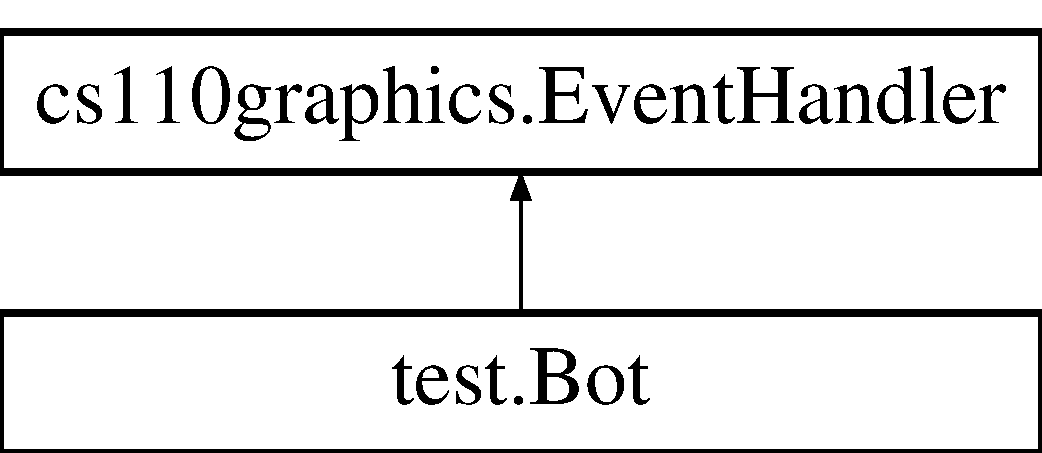
\includegraphics[height=2cm]{classtest_1_1Bot}
\end{center}
\end{figure}
\subsection*{Public Member Functions}
\begin{DoxyCompactItemize}
\item 
def \hyperlink{classtest_1_1Bot_afd02701d66ad1d70592c747a8fe4b31e}{\_\-\_\-init\_\-\_\-}
\item 
def \hyperlink{classtest_1_1Bot_a91d816dfcbfb7312349556dbae3737e6}{add\_\-to\_\-window}
\item 
def \hyperlink{classtest_1_1Bot_a23b90152ec8fa124851cd5fe6944beed}{handle\_\-key\_\-press}
\item 
def \hyperlink{classtest_1_1Bot_a173d0fff530e0987193e9006b24f218b}{handle\_\-key\_\-release}
\item 
def \hyperlink{classtest_1_1Bot_a0b184ab86d0dd6121e55394a24c8751e}{handle\_\-mouse\_\-enter}
\item 
def \hyperlink{classtest_1_1Bot_a2b65e6ecaba1afb4f117b74a684b4387}{handle\_\-mouse\_\-leave}
\item 
def \hyperlink{classtest_1_1Bot_ad1464516fb04013fa7e353a78f0ec218}{handle\_\-mouse\_\-move}
\item 
def \hyperlink{classtest_1_1Bot_a970422a4391cc2b9ff89a2e42063bb6e}{handle\_\-mouse\_\-press}
\item 
def \hyperlink{classtest_1_1Bot_a18fc05b6e2c1e42e1b6c639f4844a059}{handle\_\-mouse\_\-release}
\end{DoxyCompactItemize}


\subsection{Detailed Description}
\begin{DoxyVerb}A bot made up of a square that detects interaction from the user. \end{DoxyVerb}
 

\subsection{Member Function Documentation}
\hypertarget{classtest_1_1Bot_afd02701d66ad1d70592c747a8fe4b31e}{
\index{test::Bot@{test::Bot}!\_\-\_\-init\_\-\_\-@{\_\-\_\-init\_\-\_\-}}
\index{\_\-\_\-init\_\-\_\-@{\_\-\_\-init\_\-\_\-}!test::Bot@{test::Bot}}
\subsubsection[{\_\-\_\-init\_\-\_\-}]{\setlength{\rightskip}{0pt plus 5cm}def test.Bot.\_\-\_\-init\_\-\_\- ( {\em self}, \/   {\em window})}}
\label{classtest_1_1Bot_afd02701d66ad1d70592c747a8fe4b31e}
\begin{DoxyVerb}Creates the bot which is comprised of one square and adds the Bot
as the event handler for the square body. \end{DoxyVerb}
 \hypertarget{classtest_1_1Bot_a91d816dfcbfb7312349556dbae3737e6}{
\index{test::Bot@{test::Bot}!add\_\-to\_\-window@{add\_\-to\_\-window}}
\index{add\_\-to\_\-window@{add\_\-to\_\-window}!test::Bot@{test::Bot}}
\subsubsection[{add\_\-to\_\-window}]{\setlength{\rightskip}{0pt plus 5cm}def test.Bot.add\_\-to\_\-window ( {\em self})}}
\label{classtest_1_1Bot_a91d816dfcbfb7312349556dbae3737e6}
\begin{DoxyVerb}This method adds the graphical representation of the bot
to the window. \end{DoxyVerb}
 \hypertarget{classtest_1_1Bot_a23b90152ec8fa124851cd5fe6944beed}{
\index{test::Bot@{test::Bot}!handle\_\-key\_\-press@{handle\_\-key\_\-press}}
\index{handle\_\-key\_\-press@{handle\_\-key\_\-press}!test::Bot@{test::Bot}}
\subsubsection[{handle\_\-key\_\-press}]{\setlength{\rightskip}{0pt plus 5cm}def test.Bot.handle\_\-key\_\-press ( {\em self}, \/   {\em event})}}
\label{classtest_1_1Bot_a23b90152ec8fa124851cd5fe6944beed}
\begin{DoxyVerb}Prints what key was pressed. This is called whenever a key is
pressed regardless of the mouse position. \end{DoxyVerb}
 

Reimplemented from \hyperlink{classcs110graphics_1_1EventHandler_af3fb3531d0b23f1430a830586cd07906}{cs110graphics.EventHandler}.\hypertarget{classtest_1_1Bot_a173d0fff530e0987193e9006b24f218b}{
\index{test::Bot@{test::Bot}!handle\_\-key\_\-release@{handle\_\-key\_\-release}}
\index{handle\_\-key\_\-release@{handle\_\-key\_\-release}!test::Bot@{test::Bot}}
\subsubsection[{handle\_\-key\_\-release}]{\setlength{\rightskip}{0pt plus 5cm}def test.Bot.handle\_\-key\_\-release ( {\em self}, \/   {\em event})}}
\label{classtest_1_1Bot_a173d0fff530e0987193e9006b24f218b}
\begin{DoxyVerb}Prints what key was released. This is called whenever a key is
pressed regardless of the mouse position. \end{DoxyVerb}
 

Reimplemented from \hyperlink{classcs110graphics_1_1EventHandler_a2849f60251baa44252992162521f2473}{cs110graphics.EventHandler}.\hypertarget{classtest_1_1Bot_a0b184ab86d0dd6121e55394a24c8751e}{
\index{test::Bot@{test::Bot}!handle\_\-mouse\_\-enter@{handle\_\-mouse\_\-enter}}
\index{handle\_\-mouse\_\-enter@{handle\_\-mouse\_\-enter}!test::Bot@{test::Bot}}
\subsubsection[{handle\_\-mouse\_\-enter}]{\setlength{\rightskip}{0pt plus 5cm}def test.Bot.handle\_\-mouse\_\-enter ( {\em self}, \/   {\em event})}}
\label{classtest_1_1Bot_a0b184ab86d0dd6121e55394a24c8751e}
\begin{DoxyVerb}Prints where the mouse entered the Bot. \end{DoxyVerb}
 

Reimplemented from \hyperlink{classcs110graphics_1_1EventHandler_a13af3268f8a1aa36b8483eb2deffef15}{cs110graphics.EventHandler}.\hypertarget{classtest_1_1Bot_a2b65e6ecaba1afb4f117b74a684b4387}{
\index{test::Bot@{test::Bot}!handle\_\-mouse\_\-leave@{handle\_\-mouse\_\-leave}}
\index{handle\_\-mouse\_\-leave@{handle\_\-mouse\_\-leave}!test::Bot@{test::Bot}}
\subsubsection[{handle\_\-mouse\_\-leave}]{\setlength{\rightskip}{0pt plus 5cm}def test.Bot.handle\_\-mouse\_\-leave ( {\em self}, \/   {\em event})}}
\label{classtest_1_1Bot_a2b65e6ecaba1afb4f117b74a684b4387}
\begin{DoxyVerb}Prints where the mouse left the Bot. \end{DoxyVerb}
 

Reimplemented from \hyperlink{classcs110graphics_1_1EventHandler_a5deaf2b6b8055e97ac0ddf6603132c64}{cs110graphics.EventHandler}.\hypertarget{classtest_1_1Bot_ad1464516fb04013fa7e353a78f0ec218}{
\index{test::Bot@{test::Bot}!handle\_\-mouse\_\-move@{handle\_\-mouse\_\-move}}
\index{handle\_\-mouse\_\-move@{handle\_\-mouse\_\-move}!test::Bot@{test::Bot}}
\subsubsection[{handle\_\-mouse\_\-move}]{\setlength{\rightskip}{0pt plus 5cm}def test.Bot.handle\_\-mouse\_\-move ( {\em self}, \/   {\em event})}}
\label{classtest_1_1Bot_ad1464516fb04013fa7e353a78f0ec218}
\begin{DoxyVerb}Prints when the mouse moves while on the Bot. \end{DoxyVerb}
 

Reimplemented from \hyperlink{classcs110graphics_1_1EventHandler_a521fdcd170d15c0b8baa124c78b6d1ef}{cs110graphics.EventHandler}.\hypertarget{classtest_1_1Bot_a970422a4391cc2b9ff89a2e42063bb6e}{
\index{test::Bot@{test::Bot}!handle\_\-mouse\_\-press@{handle\_\-mouse\_\-press}}
\index{handle\_\-mouse\_\-press@{handle\_\-mouse\_\-press}!test::Bot@{test::Bot}}
\subsubsection[{handle\_\-mouse\_\-press}]{\setlength{\rightskip}{0pt plus 5cm}def test.Bot.handle\_\-mouse\_\-press ( {\em self}, \/   {\em event})}}
\label{classtest_1_1Bot_a970422a4391cc2b9ff89a2e42063bb6e}
\begin{DoxyVerb}Prints where the mouse was pressed while on the Bot. \end{DoxyVerb}
 

Reimplemented from \hyperlink{classcs110graphics_1_1EventHandler_a547873123ebcd3fcc63a2e03d2a2fee3}{cs110graphics.EventHandler}.\hypertarget{classtest_1_1Bot_a18fc05b6e2c1e42e1b6c639f4844a059}{
\index{test::Bot@{test::Bot}!handle\_\-mouse\_\-release@{handle\_\-mouse\_\-release}}
\index{handle\_\-mouse\_\-release@{handle\_\-mouse\_\-release}!test::Bot@{test::Bot}}
\subsubsection[{handle\_\-mouse\_\-release}]{\setlength{\rightskip}{0pt plus 5cm}def test.Bot.handle\_\-mouse\_\-release ( {\em self}, \/   {\em event})}}
\label{classtest_1_1Bot_a18fc05b6e2c1e42e1b6c639f4844a059}
\begin{DoxyVerb}Prints where the mouse was released while on the Bot. \end{DoxyVerb}
 

Reimplemented from \hyperlink{classcs110graphics_1_1EventHandler_a320a7dbf68d37e0101b237bff1713088}{cs110graphics.EventHandler}.

The documentation for this class was generated from the following file:\begin{DoxyCompactItemize}
\item 
test.py\end{DoxyCompactItemize}

\hypertarget{classcs110graphics_1_1Circle}{
\section{cs110graphics.Circle Class Reference}
\label{classcs110graphics_1_1Circle}\index{cs110graphics::Circle@{cs110graphics::Circle}}
}


A circle, which can be added to a \hyperlink{classcs110graphics_1_1Window}{Window} object.  
Inheritance diagram for cs110graphics.Circle::\begin{figure}[H]
\begin{center}
\leavevmode
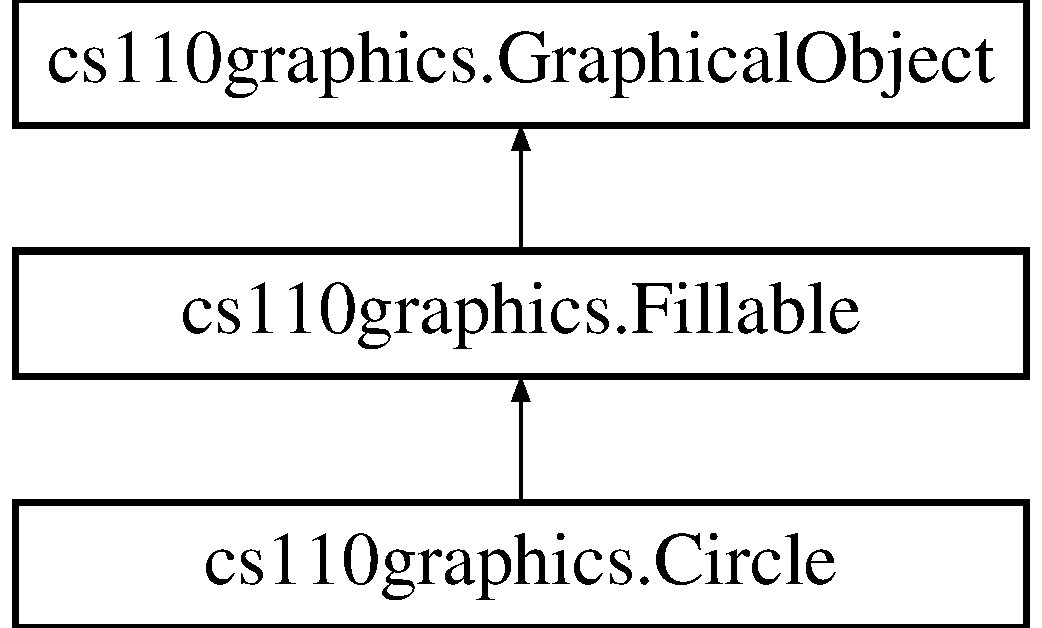
\includegraphics[height=3cm]{classcs110graphics_1_1Circle}
\end{center}
\end{figure}
\subsection*{Public Member Functions}
\begin{DoxyCompactItemize}
\item 
def \hyperlink{classcs110graphics_1_1Circle_a7c92c173c0e9666d0682c48fbd170e9f}{\_\-\_\-init\_\-\_\-}
\item 
def \hyperlink{classcs110graphics_1_1Circle_a39b0cb138b31565d2a52180a2b03cc31}{set\_\-radius}
\begin{DoxyCompactList}\small\item\em Sets the radius of the \hyperlink{classcs110graphics_1_1Circle}{Circle}. \item\end{DoxyCompactList}\item 
def \hyperlink{classcs110graphics_1_1Fillable_a6772d56158c9fe98a33f01d47cb8aa41}{get\_\-border\_\-color}
\begin{DoxyCompactList}\small\item\em Returns the border color. \item\end{DoxyCompactList}\item 
def \hyperlink{classcs110graphics_1_1Fillable_a6ed7a4288e84a090ec185c8bdff21d0f}{get\_\-border\_\-width}
\begin{DoxyCompactList}\small\item\em Returns the border width. \item\end{DoxyCompactList}\item 
def \hyperlink{classcs110graphics_1_1Fillable_a16c045bc9b63961b696914ee1a1d14d9}{get\_\-fill\_\-color}
\begin{DoxyCompactList}\small\item\em Returns fill color. \item\end{DoxyCompactList}\item 
def \hyperlink{classcs110graphics_1_1Fillable_a514fa0d21297c1372681afae9219fd58}{get\_\-pivot}
\begin{DoxyCompactList}\small\item\em Returns the pivot point. \item\end{DoxyCompactList}\item 
def \hyperlink{classcs110graphics_1_1Fillable_afa6710f6c314de39d19f06d9dd306d7d}{rotate}
\begin{DoxyCompactList}\small\item\em Rotates the object. \item\end{DoxyCompactList}\item 
def \hyperlink{classcs110graphics_1_1Fillable_a80d5b6b6d2ebae867dccecb803075749}{scale}
\begin{DoxyCompactList}\small\item\em Scales the object up or down depending on the factor. \item\end{DoxyCompactList}\item 
def \hyperlink{classcs110graphics_1_1Fillable_ae8f6c476e29c0810453dc16948e1730c}{move}
\begin{DoxyCompactList}\small\item\em Moves the object dx pixels horizontally and dy pixels vertically. \item\end{DoxyCompactList}\item 
def \hyperlink{classcs110graphics_1_1Fillable_adcabc14e76d1160ff591b9ef7f3d6a97}{move\_\-to}
\begin{DoxyCompactList}\small\item\em Moves a graphical object to a point. \item\end{DoxyCompactList}\item 
def \hyperlink{classcs110graphics_1_1Fillable_a2f830be5d970faac97759910d20d68a4}{set\_\-border\_\-color}
\begin{DoxyCompactList}\small\item\em Sets the border color. \item\end{DoxyCompactList}\item 
def \hyperlink{classcs110graphics_1_1Fillable_a09f05462cb2ed38fdccb244340f05b2b}{set\_\-border\_\-width}
\begin{DoxyCompactList}\small\item\em Sets the border width. \item\end{DoxyCompactList}\item 
def \hyperlink{classcs110graphics_1_1Fillable_a4f24c7186c8d057e42a0209eb1d56be7}{set\_\-fill\_\-color}
\begin{DoxyCompactList}\small\item\em Sets the fill color. \item\end{DoxyCompactList}\item 
def \hyperlink{classcs110graphics_1_1Fillable_a2a6066d1a11c0854ff5ee85e7d9ceb54}{set\_\-pivot}
\begin{DoxyCompactList}\small\item\em Sets the pivot point. \item\end{DoxyCompactList}\item 
def \hyperlink{classcs110graphics_1_1GraphicalObject_adb1af0d5a6baae3f9a08d21a3227c49f}{add\_\-handler}
\begin{DoxyCompactList}\small\item\em Adds a handler to the graphical object. \item\end{DoxyCompactList}\item 
def \hyperlink{classcs110graphics_1_1GraphicalObject_a062789c4cc9de38af32dcc4ff2058607}{get\_\-center}
\begin{DoxyCompactList}\small\item\em Returns the center of the object. \item\end{DoxyCompactList}\item 
def \hyperlink{classcs110graphics_1_1GraphicalObject_a6d9f5718cd0cf249e0d2842971bae17f}{get\_\-depth}
\begin{DoxyCompactList}\small\item\em Returns the depth of the object. \item\end{DoxyCompactList}\item 
def \hyperlink{classcs110graphics_1_1GraphicalObject_a20d76d4ee4419c3065d61deb6cbc6700}{set\_\-depth}
\begin{DoxyCompactList}\small\item\em Sets the depth of the \hyperlink{classcs110graphics_1_1GraphicalObject}{GraphicalObject}. \item\end{DoxyCompactList}\end{DoxyCompactItemize}


\subsection{Detailed Description}
A circle, which can be added to a \hyperlink{classcs110graphics_1_1Window}{Window} object. 

\subsection{Member Function Documentation}
\hypertarget{classcs110graphics_1_1Circle_a7c92c173c0e9666d0682c48fbd170e9f}{
\index{cs110graphics::Circle@{cs110graphics::Circle}!\_\-\_\-init\_\-\_\-@{\_\-\_\-init\_\-\_\-}}
\index{\_\-\_\-init\_\-\_\-@{\_\-\_\-init\_\-\_\-}!cs110graphics::Circle@{cs110graphics::Circle}}
\subsubsection[{\_\-\_\-init\_\-\_\-}]{\setlength{\rightskip}{0pt plus 5cm}def cs110graphics.Circle.\_\-\_\-init\_\-\_\- ( {\em self}, \/   {\em window}, \/   {\em radius} = {\ttfamily 40}, \/   {\em center} = {\ttfamily (200,~200})}}
\label{classcs110graphics_1_1Circle_a7c92c173c0e9666d0682c48fbd170e9f}

\begin{DoxyParams}{Parameters}
\item[{\em window}]-\/ \hyperlink{classcs110graphics_1_1Window}{Window} -\/ the window which the object will be added to \item[{\em radius}]-\/ int -\/ {\bfseries (default: 40)} the radius of the circle \item[{\em center}]-\/ tuple of (int $\ast$ int) -\/ {\bfseries (default: (200, 200))} sets the center of the circle \end{DoxyParams}
\hypertarget{classcs110graphics_1_1GraphicalObject_adb1af0d5a6baae3f9a08d21a3227c49f}{
\index{cs110graphics::Circle@{cs110graphics::Circle}!add\_\-handler@{add\_\-handler}}
\index{add\_\-handler@{add\_\-handler}!cs110graphics::Circle@{cs110graphics::Circle}}
\subsubsection[{add\_\-handler}]{\setlength{\rightskip}{0pt plus 5cm}def cs110graphics.GraphicalObject.add\_\-handler ( {\em self}, \/   {\em handler\_\-object})\hspace{0.3cm}{\ttfamily  \mbox{[}inherited\mbox{]}}}}
\label{classcs110graphics_1_1GraphicalObject_adb1af0d5a6baae3f9a08d21a3227c49f}


Adds a handler to the graphical object. 
\begin{DoxyParams}{Parameters}
\item[{\em handler\_\-object}]-\/ \hyperlink{classcs110graphics_1_1EventHandler}{EventHandler} -\/ the object that handles the events for this \hyperlink{classcs110graphics_1_1GraphicalObject}{GraphicalObject} \end{DoxyParams}
\hypertarget{classcs110graphics_1_1Fillable_a6772d56158c9fe98a33f01d47cb8aa41}{
\index{cs110graphics::Circle@{cs110graphics::Circle}!get\_\-border\_\-color@{get\_\-border\_\-color}}
\index{get\_\-border\_\-color@{get\_\-border\_\-color}!cs110graphics::Circle@{cs110graphics::Circle}}
\subsubsection[{get\_\-border\_\-color}]{\setlength{\rightskip}{0pt plus 5cm}def cs110graphics.Fillable.get\_\-border\_\-color ( {\em self})\hspace{0.3cm}{\ttfamily  \mbox{[}inherited\mbox{]}}}}
\label{classcs110graphics_1_1Fillable_a6772d56158c9fe98a33f01d47cb8aa41}


Returns the border color. \begin{DoxyReturn}{Returns}
border\_\-color -\/ str -\/ Can be either the name of a color (\char`\"{}yellow\char`\"{}), or a hex code (\char`\"{}\#FFFF00\char`\"{}) 
\end{DoxyReturn}
\hypertarget{classcs110graphics_1_1Fillable_a6ed7a4288e84a090ec185c8bdff21d0f}{
\index{cs110graphics::Circle@{cs110graphics::Circle}!get\_\-border\_\-width@{get\_\-border\_\-width}}
\index{get\_\-border\_\-width@{get\_\-border\_\-width}!cs110graphics::Circle@{cs110graphics::Circle}}
\subsubsection[{get\_\-border\_\-width}]{\setlength{\rightskip}{0pt plus 5cm}def cs110graphics.Fillable.get\_\-border\_\-width ( {\em self})\hspace{0.3cm}{\ttfamily  \mbox{[}inherited\mbox{]}}}}
\label{classcs110graphics_1_1Fillable_a6ed7a4288e84a090ec185c8bdff21d0f}


Returns the border width. \begin{DoxyReturn}{Returns}
border\_\-width -\/ int 
\end{DoxyReturn}
\hypertarget{classcs110graphics_1_1GraphicalObject_a062789c4cc9de38af32dcc4ff2058607}{
\index{cs110graphics::Circle@{cs110graphics::Circle}!get\_\-center@{get\_\-center}}
\index{get\_\-center@{get\_\-center}!cs110graphics::Circle@{cs110graphics::Circle}}
\subsubsection[{get\_\-center}]{\setlength{\rightskip}{0pt plus 5cm}def cs110graphics.GraphicalObject.get\_\-center ( {\em self})\hspace{0.3cm}{\ttfamily  \mbox{[}inherited\mbox{]}}}}
\label{classcs110graphics_1_1GraphicalObject_a062789c4cc9de38af32dcc4ff2058607}


Returns the center of the object. \begin{DoxyReturn}{Returns}
center -\/ tuple 
\end{DoxyReturn}
\hypertarget{classcs110graphics_1_1GraphicalObject_a6d9f5718cd0cf249e0d2842971bae17f}{
\index{cs110graphics::Circle@{cs110graphics::Circle}!get\_\-depth@{get\_\-depth}}
\index{get\_\-depth@{get\_\-depth}!cs110graphics::Circle@{cs110graphics::Circle}}
\subsubsection[{get\_\-depth}]{\setlength{\rightskip}{0pt plus 5cm}def cs110graphics.GraphicalObject.get\_\-depth ( {\em self})\hspace{0.3cm}{\ttfamily  \mbox{[}inherited\mbox{]}}}}
\label{classcs110graphics_1_1GraphicalObject_a6d9f5718cd0cf249e0d2842971bae17f}


Returns the depth of the object. \begin{DoxyReturn}{Returns}
depth -\/ int 
\end{DoxyReturn}
\hypertarget{classcs110graphics_1_1Fillable_a16c045bc9b63961b696914ee1a1d14d9}{
\index{cs110graphics::Circle@{cs110graphics::Circle}!get\_\-fill\_\-color@{get\_\-fill\_\-color}}
\index{get\_\-fill\_\-color@{get\_\-fill\_\-color}!cs110graphics::Circle@{cs110graphics::Circle}}
\subsubsection[{get\_\-fill\_\-color}]{\setlength{\rightskip}{0pt plus 5cm}def cs110graphics.Fillable.get\_\-fill\_\-color ( {\em self})\hspace{0.3cm}{\ttfamily  \mbox{[}inherited\mbox{]}}}}
\label{classcs110graphics_1_1Fillable_a16c045bc9b63961b696914ee1a1d14d9}


Returns fill color. \begin{DoxyReturn}{Returns}
color -\/ int -\/ Can be either the name of a color (\char`\"{}yellow\char`\"{}), or a hex code (\char`\"{}\#FFFF00\char`\"{}) 
\end{DoxyReturn}
\hypertarget{classcs110graphics_1_1Fillable_a514fa0d21297c1372681afae9219fd58}{
\index{cs110graphics::Circle@{cs110graphics::Circle}!get\_\-pivot@{get\_\-pivot}}
\index{get\_\-pivot@{get\_\-pivot}!cs110graphics::Circle@{cs110graphics::Circle}}
\subsubsection[{get\_\-pivot}]{\setlength{\rightskip}{0pt plus 5cm}def cs110graphics.Fillable.get\_\-pivot ( {\em self})\hspace{0.3cm}{\ttfamily  \mbox{[}inherited\mbox{]}}}}
\label{classcs110graphics_1_1Fillable_a514fa0d21297c1372681afae9219fd58}


Returns the pivot point. \begin{DoxyReturn}{Returns}
pivot -\/ tuple (int $\ast$ int) 
\end{DoxyReturn}
\hypertarget{classcs110graphics_1_1Fillable_ae8f6c476e29c0810453dc16948e1730c}{
\index{cs110graphics::Circle@{cs110graphics::Circle}!move@{move}}
\index{move@{move}!cs110graphics::Circle@{cs110graphics::Circle}}
\subsubsection[{move}]{\setlength{\rightskip}{0pt plus 5cm}def cs110graphics.Fillable.move ( {\em self}, \/   {\em dx}, \/   {\em dy})\hspace{0.3cm}{\ttfamily  \mbox{[}inherited\mbox{]}}}}
\label{classcs110graphics_1_1Fillable_ae8f6c476e29c0810453dc16948e1730c}


Moves the object dx pixels horizontally and dy pixels vertically. 
\begin{DoxyParams}{Parameters}
\item[{\em dx}]-\/ int \item[{\em dy}]-\/ int \end{DoxyParams}


Reimplemented from \hyperlink{classcs110graphics_1_1GraphicalObject_aa64d270fb83efa4a54e1a7953512f9cd}{cs110graphics.GraphicalObject}.\hypertarget{classcs110graphics_1_1Fillable_adcabc14e76d1160ff591b9ef7f3d6a97}{
\index{cs110graphics::Circle@{cs110graphics::Circle}!move\_\-to@{move\_\-to}}
\index{move\_\-to@{move\_\-to}!cs110graphics::Circle@{cs110graphics::Circle}}
\subsubsection[{move\_\-to}]{\setlength{\rightskip}{0pt plus 5cm}def cs110graphics.Fillable.move\_\-to ( {\em self}, \/   {\em point})\hspace{0.3cm}{\ttfamily  \mbox{[}inherited\mbox{]}}}}
\label{classcs110graphics_1_1Fillable_adcabc14e76d1160ff591b9ef7f3d6a97}


Moves a graphical object to a point. 
\begin{DoxyParams}{Parameters}
\item[{\em point}]-\/ tuple of (int $\ast$ int) \end{DoxyParams}


Reimplemented from \hyperlink{classcs110graphics_1_1GraphicalObject_abe2d480265df7ac9447205c52c6946df}{cs110graphics.GraphicalObject}.\hypertarget{classcs110graphics_1_1Fillable_afa6710f6c314de39d19f06d9dd306d7d}{
\index{cs110graphics::Circle@{cs110graphics::Circle}!rotate@{rotate}}
\index{rotate@{rotate}!cs110graphics::Circle@{cs110graphics::Circle}}
\subsubsection[{rotate}]{\setlength{\rightskip}{0pt plus 5cm}def cs110graphics.Fillable.rotate ( {\em self}, \/   {\em degrees})\hspace{0.3cm}{\ttfamily  \mbox{[}inherited\mbox{]}}}}
\label{classcs110graphics_1_1Fillable_afa6710f6c314de39d19f06d9dd306d7d}


Rotates the object. 
\begin{DoxyParams}{Parameters}
\item[{\em degrees}]-\/ int \end{DoxyParams}
\hypertarget{classcs110graphics_1_1Fillable_a80d5b6b6d2ebae867dccecb803075749}{
\index{cs110graphics::Circle@{cs110graphics::Circle}!scale@{scale}}
\index{scale@{scale}!cs110graphics::Circle@{cs110graphics::Circle}}
\subsubsection[{scale}]{\setlength{\rightskip}{0pt plus 5cm}def cs110graphics.Fillable.scale ( {\em self}, \/   {\em factor})\hspace{0.3cm}{\ttfamily  \mbox{[}inherited\mbox{]}}}}
\label{classcs110graphics_1_1Fillable_a80d5b6b6d2ebae867dccecb803075749}


Scales the object up or down depending on the factor. 
\begin{DoxyParams}{Parameters}
\item[{\em factor}]-\/ float \end{DoxyParams}
\hypertarget{classcs110graphics_1_1Fillable_a2f830be5d970faac97759910d20d68a4}{
\index{cs110graphics::Circle@{cs110graphics::Circle}!set\_\-border\_\-color@{set\_\-border\_\-color}}
\index{set\_\-border\_\-color@{set\_\-border\_\-color}!cs110graphics::Circle@{cs110graphics::Circle}}
\subsubsection[{set\_\-border\_\-color}]{\setlength{\rightskip}{0pt plus 5cm}def cs110graphics.Fillable.set\_\-border\_\-color ( {\em self}, \/   {\em color})\hspace{0.3cm}{\ttfamily  \mbox{[}inherited\mbox{]}}}}
\label{classcs110graphics_1_1Fillable_a2f830be5d970faac97759910d20d68a4}


Sets the border color. 
\begin{DoxyParams}{Parameters}
\item[{\em color}]-\/ string -\/ Can be either the name of a color (\char`\"{}yellow\char`\"{}), or a hex code (\char`\"{}\#FFFF00\char`\"{}) \end{DoxyParams}
\hypertarget{classcs110graphics_1_1Fillable_a09f05462cb2ed38fdccb244340f05b2b}{
\index{cs110graphics::Circle@{cs110graphics::Circle}!set\_\-border\_\-width@{set\_\-border\_\-width}}
\index{set\_\-border\_\-width@{set\_\-border\_\-width}!cs110graphics::Circle@{cs110graphics::Circle}}
\subsubsection[{set\_\-border\_\-width}]{\setlength{\rightskip}{0pt plus 5cm}def cs110graphics.Fillable.set\_\-border\_\-width ( {\em self}, \/   {\em width})\hspace{0.3cm}{\ttfamily  \mbox{[}inherited\mbox{]}}}}
\label{classcs110graphics_1_1Fillable_a09f05462cb2ed38fdccb244340f05b2b}


Sets the border width. 
\begin{DoxyParams}{Parameters}
\item[{\em width}]-\/ int \end{DoxyParams}
\hypertarget{classcs110graphics_1_1GraphicalObject_a20d76d4ee4419c3065d61deb6cbc6700}{
\index{cs110graphics::Circle@{cs110graphics::Circle}!set\_\-depth@{set\_\-depth}}
\index{set\_\-depth@{set\_\-depth}!cs110graphics::Circle@{cs110graphics::Circle}}
\subsubsection[{set\_\-depth}]{\setlength{\rightskip}{0pt plus 5cm}def cs110graphics.GraphicalObject.set\_\-depth ( {\em self}, \/   {\em depth})\hspace{0.3cm}{\ttfamily  \mbox{[}inherited\mbox{]}}}}
\label{classcs110graphics_1_1GraphicalObject_a20d76d4ee4419c3065d61deb6cbc6700}


Sets the depth of the \hyperlink{classcs110graphics_1_1GraphicalObject}{GraphicalObject}. 
\begin{DoxyParams}{Parameters}
\item[{\em depth}]-\/ int \end{DoxyParams}
\hypertarget{classcs110graphics_1_1Fillable_a4f24c7186c8d057e42a0209eb1d56be7}{
\index{cs110graphics::Circle@{cs110graphics::Circle}!set\_\-fill\_\-color@{set\_\-fill\_\-color}}
\index{set\_\-fill\_\-color@{set\_\-fill\_\-color}!cs110graphics::Circle@{cs110graphics::Circle}}
\subsubsection[{set\_\-fill\_\-color}]{\setlength{\rightskip}{0pt plus 5cm}def cs110graphics.Fillable.set\_\-fill\_\-color ( {\em self}, \/   {\em color})\hspace{0.3cm}{\ttfamily  \mbox{[}inherited\mbox{]}}}}
\label{classcs110graphics_1_1Fillable_a4f24c7186c8d057e42a0209eb1d56be7}


Sets the fill color. 
\begin{DoxyParams}{Parameters}
\item[{\em color}]-\/ string -\/ Can be either the name of a color (\char`\"{}yellow\char`\"{}), or a hex code (\char`\"{}\#FFFF00\char`\"{}) \end{DoxyParams}
\hypertarget{classcs110graphics_1_1Fillable_a2a6066d1a11c0854ff5ee85e7d9ceb54}{
\index{cs110graphics::Circle@{cs110graphics::Circle}!set\_\-pivot@{set\_\-pivot}}
\index{set\_\-pivot@{set\_\-pivot}!cs110graphics::Circle@{cs110graphics::Circle}}
\subsubsection[{set\_\-pivot}]{\setlength{\rightskip}{0pt plus 5cm}def cs110graphics.Fillable.set\_\-pivot ( {\em self}, \/   {\em pivot})\hspace{0.3cm}{\ttfamily  \mbox{[}inherited\mbox{]}}}}
\label{classcs110graphics_1_1Fillable_a2a6066d1a11c0854ff5ee85e7d9ceb54}


Sets the pivot point. 
\begin{DoxyParams}{Parameters}
\item[{\em pivot}]-\/ tuple of (int $\ast$ int) \end{DoxyParams}
\hypertarget{classcs110graphics_1_1Circle_a39b0cb138b31565d2a52180a2b03cc31}{
\index{cs110graphics::Circle@{cs110graphics::Circle}!set\_\-radius@{set\_\-radius}}
\index{set\_\-radius@{set\_\-radius}!cs110graphics::Circle@{cs110graphics::Circle}}
\subsubsection[{set\_\-radius}]{\setlength{\rightskip}{0pt plus 5cm}def cs110graphics.Circle.set\_\-radius ( {\em self}, \/   {\em radius})}}
\label{classcs110graphics_1_1Circle_a39b0cb138b31565d2a52180a2b03cc31}


Sets the radius of the \hyperlink{classcs110graphics_1_1Circle}{Circle}. 
\begin{DoxyParams}{Parameters}
\item[{\em radius}]-\/ int \end{DoxyParams}


The documentation for this class was generated from the following file:\begin{DoxyCompactItemize}
\item 
\hyperlink{cs110graphics_8py}{cs110graphics.py}\end{DoxyCompactItemize}

\hypertarget{classcs110graphics_1_1Event}{
\section{cs110graphics.Event Class Reference}
\label{classcs110graphics_1_1Event}\index{cs110graphics::Event@{cs110graphics::Event}}
}


An object representing an action from the user.  
\subsection*{Public Member Functions}
\begin{DoxyCompactItemize}
\item 
def \hyperlink{classcs110graphics_1_1Event_abdb7a2999936cc7ab1119289f05f8243}{get\_\-button}
\begin{DoxyCompactList}\small\item\em Returns the mouse button that is attached to the event. \item\end{DoxyCompactList}\item 
def \hyperlink{classcs110graphics_1_1Event_a7bd201ecbf74db6d78dbf2fb4f622a7c}{get\_\-description}
\begin{DoxyCompactList}\small\item\em Returns the description of the event. \item\end{DoxyCompactList}\item 
def \hyperlink{classcs110graphics_1_1Event_a0d795ddaef92049cee1d7b09898cf225}{get\_\-key}
\begin{DoxyCompactList}\small\item\em Returns the keyboard key that is attached to the event. \item\end{DoxyCompactList}\item 
def \hyperlink{classcs110graphics_1_1Event_a2db4866adee7a6ddb8d32240801fb8ce}{get\_\-mouse\_\-location}
\begin{DoxyCompactList}\small\item\em Returns a tuple of the x and y coordinates of the mouse location in the canvas. \item\end{DoxyCompactList}\item 
def \hyperlink{classcs110graphics_1_1Event_a7c8fb2d5e9288db125801d5a6e66ecf1}{get\_\-root\_\-mouse\_\-location}
\begin{DoxyCompactList}\small\item\em Returns a tuple of the x and y coordinates of the mouse location in the window. \item\end{DoxyCompactList}\end{DoxyCompactItemize}


\subsection{Detailed Description}
An object representing an action from the user. Used by \hyperlink{classcs110graphics_1_1EventHandler}{EventHandler} objects. User actions that create \hyperlink{classcs110graphics_1_1Event}{Event} objects include:
\begin{DoxyItemize}
\item Pressing/Releasing a key on the keyboard
\item Pressing/Releasing a button on the mouse while on a \hyperlink{classcs110graphics_1_1GraphicalObject}{GraphicalObject} with an event handler
\item Moving the mouse while on a \hyperlink{classcs110graphics_1_1GraphicalObject}{GraphicalObject} with an event handler
\end{DoxyItemize}

Each of these actions will call their corresponding methods in \hyperlink{classcs110graphics_1_1EventHandler}{EventHandler} automatically and give an instance of \hyperlink{classcs110graphics_1_1Event}{Event} to the method called. 

\subsection{Member Function Documentation}
\hypertarget{classcs110graphics_1_1Event_abdb7a2999936cc7ab1119289f05f8243}{
\index{cs110graphics::Event@{cs110graphics::Event}!get\_\-button@{get\_\-button}}
\index{get\_\-button@{get\_\-button}!cs110graphics::Event@{cs110graphics::Event}}
\subsubsection[{get\_\-button}]{\setlength{\rightskip}{0pt plus 5cm}def cs110graphics.Event.get\_\-button ( {\em self})}}
\label{classcs110graphics_1_1Event_abdb7a2999936cc7ab1119289f05f8243}


Returns the mouse button that is attached to the event. Returns {\ttfamily None} if the button fails to exist (like if the \hyperlink{classcs110graphics_1_1Event}{Event} handles a key press). \begin{DoxyReturn}{Returns}
button -\/ str
\end{DoxyReturn}
Possible returns are:
\begin{DoxyItemize}
\item \char`\"{}Left Mouse Button\char`\"{}
\item \char`\"{}Right Mouse Button\char`\"{}
\item \char`\"{}Middle Mouse Button\char`\"{}
\item None 
\end{DoxyItemize}\hypertarget{classcs110graphics_1_1Event_a7bd201ecbf74db6d78dbf2fb4f622a7c}{
\index{cs110graphics::Event@{cs110graphics::Event}!get\_\-description@{get\_\-description}}
\index{get\_\-description@{get\_\-description}!cs110graphics::Event@{cs110graphics::Event}}
\subsubsection[{get\_\-description}]{\setlength{\rightskip}{0pt plus 5cm}def cs110graphics.Event.get\_\-description ( {\em self})}}
\label{classcs110graphics_1_1Event_a7bd201ecbf74db6d78dbf2fb4f622a7c}


Returns the description of the event. \begin{DoxyReturn}{Returns}
description -\/ str
\end{DoxyReturn}
Possible returns are:
\begin{DoxyItemize}
\item \char`\"{}Key Press\char`\"{}
\item \char`\"{}Key Release\char`\"{}
\item \char`\"{}Mouse Press\char`\"{}
\item \char`\"{}Mouse Release\char`\"{}
\item \char`\"{}Mouse Move\char`\"{}
\item \char`\"{}Mouse Enter\char`\"{}
\item \char`\"{}Mouse Leave\char`\"{} 
\end{DoxyItemize}\hypertarget{classcs110graphics_1_1Event_a0d795ddaef92049cee1d7b09898cf225}{
\index{cs110graphics::Event@{cs110graphics::Event}!get\_\-key@{get\_\-key}}
\index{get\_\-key@{get\_\-key}!cs110graphics::Event@{cs110graphics::Event}}
\subsubsection[{get\_\-key}]{\setlength{\rightskip}{0pt plus 5cm}def cs110graphics.Event.get\_\-key ( {\em self})}}
\label{classcs110graphics_1_1Event_a0d795ddaef92049cee1d7b09898cf225}


Returns the keyboard key that is attached to the event. Returns None if the key fails to exist (like if the \hyperlink{classcs110graphics_1_1Event}{Event} handles a mouse press). \begin{DoxyReturn}{Returns}
key -\/ str
\end{DoxyReturn}
Most keys will evaluate to a single character (eg. pressing the a-\/key will result in \char`\"{}a\char`\"{} while pressing shift-\/a will result in \char`\"{}A\char`\"{}). \hypertarget{classcs110graphics_1_1Event_a2db4866adee7a6ddb8d32240801fb8ce}{
\index{cs110graphics::Event@{cs110graphics::Event}!get\_\-mouse\_\-location@{get\_\-mouse\_\-location}}
\index{get\_\-mouse\_\-location@{get\_\-mouse\_\-location}!cs110graphics::Event@{cs110graphics::Event}}
\subsubsection[{get\_\-mouse\_\-location}]{\setlength{\rightskip}{0pt plus 5cm}def cs110graphics.Event.get\_\-mouse\_\-location ( {\em self})}}
\label{classcs110graphics_1_1Event_a2db4866adee7a6ddb8d32240801fb8ce}


Returns a tuple of the x and y coordinates of the mouse location in the canvas. \begin{DoxyReturn}{Returns}
location -\/ tuple of (int $\ast$ int) -\/ (e.g. (200, 200)) 
\end{DoxyReturn}
\hypertarget{classcs110graphics_1_1Event_a7c8fb2d5e9288db125801d5a6e66ecf1}{
\index{cs110graphics::Event@{cs110graphics::Event}!get\_\-root\_\-mouse\_\-location@{get\_\-root\_\-mouse\_\-location}}
\index{get\_\-root\_\-mouse\_\-location@{get\_\-root\_\-mouse\_\-location}!cs110graphics::Event@{cs110graphics::Event}}
\subsubsection[{get\_\-root\_\-mouse\_\-location}]{\setlength{\rightskip}{0pt plus 5cm}def cs110graphics.Event.get\_\-root\_\-mouse\_\-location ( {\em self})}}
\label{classcs110graphics_1_1Event_a7c8fb2d5e9288db125801d5a6e66ecf1}


Returns a tuple of the x and y coordinates of the mouse location in the window. Typically using get\_\-mouse\_\-location is more applicable. \begin{DoxyReturn}{Returns}
location -\/ tuple of (int $\ast$ int) -\/ (e.g. (200, 200)) 
\end{DoxyReturn}


The documentation for this class was generated from the following file:\begin{DoxyCompactItemize}
\item 
\hyperlink{cs110graphics_8py}{cs110graphics.py}\end{DoxyCompactItemize}

\hypertarget{classcs110graphics_1_1EventHandler}{
\section{cs110graphics.EventHandler Class Reference}
\label{classcs110graphics_1_1EventHandler}\index{cs110graphics::EventHandler@{cs110graphics::EventHandler}}
}


The \hyperlink{classcs110graphics_1_1EventHandler}{EventHandler} class should be extended by any class that reacts to user input in the form of some action with the computer mouse or the keyboard.  
\subsection*{Public Member Functions}
\begin{DoxyCompactItemize}
\item 
def \hyperlink{classcs110graphics_1_1EventHandler_af3fb3531d0b23f1430a830586cd07906}{handle\_\-key\_\-press}
\begin{DoxyCompactList}\small\item\em Handles a key press. \item\end{DoxyCompactList}\item 
def \hyperlink{classcs110graphics_1_1EventHandler_a2849f60251baa44252992162521f2473}{handle\_\-key\_\-release}
\begin{DoxyCompactList}\small\item\em Handles a key release. \item\end{DoxyCompactList}\item 
def \hyperlink{classcs110graphics_1_1EventHandler_a13af3268f8a1aa36b8483eb2deffef15}{handle\_\-mouse\_\-enter}
\begin{DoxyCompactList}\small\item\em Handles when a mouse enters an object. \item\end{DoxyCompactList}\item 
def \hyperlink{classcs110graphics_1_1EventHandler_a5deaf2b6b8055e97ac0ddf6603132c64}{handle\_\-mouse\_\-leave}
\begin{DoxyCompactList}\small\item\em Handles when a mouse leaves an object. \item\end{DoxyCompactList}\item 
def \hyperlink{classcs110graphics_1_1EventHandler_a521fdcd170d15c0b8baa124c78b6d1ef}{handle\_\-mouse\_\-move}
\begin{DoxyCompactList}\small\item\em Handles a mouse move. \item\end{DoxyCompactList}\item 
def \hyperlink{classcs110graphics_1_1EventHandler_a547873123ebcd3fcc63a2e03d2a2fee3}{handle\_\-mouse\_\-press}
\begin{DoxyCompactList}\small\item\em Handles a mouse press. \item\end{DoxyCompactList}\item 
def \hyperlink{classcs110graphics_1_1EventHandler_a320a7dbf68d37e0101b237bff1713088}{handle\_\-mouse\_\-release}
\begin{DoxyCompactList}\small\item\em Handles a mouse release. \item\end{DoxyCompactList}\end{DoxyCompactItemize}


\subsection{Detailed Description}
The \hyperlink{classcs110graphics_1_1EventHandler}{EventHandler} class should be extended by any class that reacts to user input in the form of some action with the computer mouse or the keyboard. Each method inherited from the \hyperlink{classcs110graphics_1_1EventHandler}{EventHandler} class takes an \hyperlink{classcs110graphics_1_1Event}{Event} object as a parameter. The methods available to \hyperlink{classcs110graphics_1_1Event}{Event} can be useful for interpreting how a call to each method should be handled. For example usage of event.get\_\-key() can be used to destinguish between the keys used in navigating a character in a game.

A sample program using the \hyperlink{classcs110graphics_1_1EventHandler}{EventHandler} is shown below. 
\begin{DoxyCode}
 from cs110graphics import *

 class Bot(EventHandler):
     """ A bot made up of a square that detects interaction from the user. """

     def __init__(self, window):
         """ Creates the bot which is comprised of one square and adds the Bot
         as the event handler for the square body. """
         self._window = window

         # create the body of the Bot and add this class
         # as the handler
         self._body = Square(window)
         self._body.add_handler(self)

     def add_to_window(self):
         """ This method adds the graphical representation of the bot
         to the window. """
         self._window.add(self._body)

     ##########################################################################
     # Event handling methods                                                  
     ##########################################################################

     def handle_key_press(self, event):
         """ Prints what key was pressed. This is called whenever a key is
         pressed regardless of the mouse position. """
         print(event.get_key(), "was pressed")

     def handle_key_release(self, event):
         """ Prints what key was released. This is called whenever a key is
         pressed regardless of the mouse position. """
         print(event.get_key(), "was released")

     def handle_mouse_enter(self, event):
         """ Prints where the mouse entered the Bot. """
         print("The mouse entered the bot at", event.get_mouse_location())

     def handle_mouse_leave(self, event):
         """ Prints where the mouse left the Bot. """
         print("The mouse left the bot at", event.get_mouse_location())

     def handle_mouse_move(self, event):
         """ Prints when the mouse moves while on the Bot. """
         print("The mouse moved to", event.get_mouse_location())

     def handle_mouse_press(self, event):
         """ Prints where the mouse was pressed while on the Bot. """
         print("The mouse was pressed at", event.get_mouse_location())

     def handle_mouse_release(self, event):
         """ Prints where the mouse was released while on the Bot. """
         print("The mouse was released at", event.get_mouse_location())

 def main(window):
     bot = Bot(window)
     bot.add_to_window()

 if __name__ == "__main__":
     StartGraphicsSystem(main)
\end{DoxyCode}
 

\subsection{Member Function Documentation}
\hypertarget{classcs110graphics_1_1EventHandler_af3fb3531d0b23f1430a830586cd07906}{
\index{cs110graphics::EventHandler@{cs110graphics::EventHandler}!handle\_\-key\_\-press@{handle\_\-key\_\-press}}
\index{handle\_\-key\_\-press@{handle\_\-key\_\-press}!cs110graphics::EventHandler@{cs110graphics::EventHandler}}
\subsubsection[{handle\_\-key\_\-press}]{\setlength{\rightskip}{0pt plus 5cm}def cs110graphics.EventHandler.handle\_\-key\_\-press ( {\em self}, \/   {\em event})}}
\label{classcs110graphics_1_1EventHandler_af3fb3531d0b23f1430a830586cd07906}


Handles a key press. This function will be called whenever a key is pressed while the window is active. The event parameter can be used to determine which key was pressed. For example: 
\begin{DoxyCode}
 class Handler(EventHandler):
     def handle_key_press(self, event):
         if "a" == event.get_key():
             # do something when a is pressed...
         else:
             # do something else...
\end{DoxyCode}
 
\begin{DoxyParams}{Parameters}
\item[{\em event}]-\/ \hyperlink{classcs110graphics_1_1Event}{Event} -\/ the event that occurred \end{DoxyParams}
\hypertarget{classcs110graphics_1_1EventHandler_a2849f60251baa44252992162521f2473}{
\index{cs110graphics::EventHandler@{cs110graphics::EventHandler}!handle\_\-key\_\-release@{handle\_\-key\_\-release}}
\index{handle\_\-key\_\-release@{handle\_\-key\_\-release}!cs110graphics::EventHandler@{cs110graphics::EventHandler}}
\subsubsection[{handle\_\-key\_\-release}]{\setlength{\rightskip}{0pt plus 5cm}def cs110graphics.EventHandler.handle\_\-key\_\-release ( {\em self}, \/   {\em event})}}
\label{classcs110graphics_1_1EventHandler_a2849f60251baa44252992162521f2473}


Handles a key release. This method will be called whenever a key is released while the window is active. The event parameter can be used to determine which key was pressed. For example: 
\begin{DoxyCode}
 class Handler(EventHandler):
     def handle_key_release(self, event):
         if "a" == event.get_key():
             # do something when a is released...
         else:
             # do something else...
\end{DoxyCode}
 
\begin{DoxyParams}{Parameters}
\item[{\em event}]-\/ \hyperlink{classcs110graphics_1_1Event}{Event} -\/ the event that occurred \end{DoxyParams}
\hypertarget{classcs110graphics_1_1EventHandler_a13af3268f8a1aa36b8483eb2deffef15}{
\index{cs110graphics::EventHandler@{cs110graphics::EventHandler}!handle\_\-mouse\_\-enter@{handle\_\-mouse\_\-enter}}
\index{handle\_\-mouse\_\-enter@{handle\_\-mouse\_\-enter}!cs110graphics::EventHandler@{cs110graphics::EventHandler}}
\subsubsection[{handle\_\-mouse\_\-enter}]{\setlength{\rightskip}{0pt plus 5cm}def cs110graphics.EventHandler.handle\_\-mouse\_\-enter ( {\em self}, \/   {\em event})}}
\label{classcs110graphics_1_1EventHandler_a13af3268f8a1aa36b8483eb2deffef15}


Handles when a mouse enters an object. \begin{Desc}
\item[\hyperlink{bug__bug000001}{Bug}]Overrides of this method is likely to be called more often than expected and many \hyperlink{classcs110graphics_1_1GraphicalObject}{GraphicalObject} methods will not work correctly with when called within the method, avoid using this if possible.\end{Desc}
This is called by the system when the mouse enters the \hyperlink{classcs110graphics_1_1GraphicalObject}{GraphicalObject} that this handler is an event handler for. The event parameter can be used to determine the location at which the mouse entered the object. 
\begin{DoxyCode}
 class Handler(EventHandler):
     def handle_mouse_enter(self, event):
         mouse_location = event.get_mouse_location()
\end{DoxyCode}
 
\begin{DoxyParams}{Parameters}
\item[{\em event}]-\/ \hyperlink{classcs110graphics_1_1Event}{Event} -\/ the event that occurred \end{DoxyParams}
\hypertarget{classcs110graphics_1_1EventHandler_a5deaf2b6b8055e97ac0ddf6603132c64}{
\index{cs110graphics::EventHandler@{cs110graphics::EventHandler}!handle\_\-mouse\_\-leave@{handle\_\-mouse\_\-leave}}
\index{handle\_\-mouse\_\-leave@{handle\_\-mouse\_\-leave}!cs110graphics::EventHandler@{cs110graphics::EventHandler}}
\subsubsection[{handle\_\-mouse\_\-leave}]{\setlength{\rightskip}{0pt plus 5cm}def cs110graphics.EventHandler.handle\_\-mouse\_\-leave ( {\em self}, \/   {\em event})}}
\label{classcs110graphics_1_1EventHandler_a5deaf2b6b8055e97ac0ddf6603132c64}


Handles when a mouse leaves an object. This is called by the system when the mouse leaves the \hyperlink{classcs110graphics_1_1GraphicalObject}{GraphicalObject} that this handler is an event handler for. The event parameter can be used to determine the location at which the mouse left the object. 
\begin{DoxyCode}
 class Handler(EventHandler):
     def handle_mouse_leave(self, event):
         mouse_location = event.get_mouse_location()
\end{DoxyCode}
 
\begin{DoxyParams}{Parameters}
\item[{\em event}]-\/ \hyperlink{classcs110graphics_1_1Event}{Event} -\/ the event that occurred \end{DoxyParams}
\hypertarget{classcs110graphics_1_1EventHandler_a521fdcd170d15c0b8baa124c78b6d1ef}{
\index{cs110graphics::EventHandler@{cs110graphics::EventHandler}!handle\_\-mouse\_\-move@{handle\_\-mouse\_\-move}}
\index{handle\_\-mouse\_\-move@{handle\_\-mouse\_\-move}!cs110graphics::EventHandler@{cs110graphics::EventHandler}}
\subsubsection[{handle\_\-mouse\_\-move}]{\setlength{\rightskip}{0pt plus 5cm}def cs110graphics.EventHandler.handle\_\-mouse\_\-move ( {\em self}, \/   {\em event})}}
\label{classcs110graphics_1_1EventHandler_a521fdcd170d15c0b8baa124c78b6d1ef}


Handles a mouse move. This is called by the system when the mouse moves within the \hyperlink{classcs110graphics_1_1GraphicalObject}{GraphicalObject} that this handler is an event handler for. The event parameter can be used to determine the location that the mouse moved to. 
\begin{DoxyCode}
 class Handler(EventHandler):
     def handle_mouse_move(self, event):
         mouse_location = event.get_mouse_location()
\end{DoxyCode}
 
\begin{DoxyParams}{Parameters}
\item[{\em event}]-\/ \hyperlink{classcs110graphics_1_1Event}{Event} -\/ the event that occurred \end{DoxyParams}
\hypertarget{classcs110graphics_1_1EventHandler_a547873123ebcd3fcc63a2e03d2a2fee3}{
\index{cs110graphics::EventHandler@{cs110graphics::EventHandler}!handle\_\-mouse\_\-press@{handle\_\-mouse\_\-press}}
\index{handle\_\-mouse\_\-press@{handle\_\-mouse\_\-press}!cs110graphics::EventHandler@{cs110graphics::EventHandler}}
\subsubsection[{handle\_\-mouse\_\-press}]{\setlength{\rightskip}{0pt plus 5cm}def cs110graphics.EventHandler.handle\_\-mouse\_\-press ( {\em self}, \/   {\em event})}}
\label{classcs110graphics_1_1EventHandler_a547873123ebcd3fcc63a2e03d2a2fee3}


Handles a mouse press. \begin{Desc}
\item[\hyperlink{bug__bug000002}{Bug}]GraphicalObjects may not update correctly if moved or modified within this method. You can use this for setting variables, though.\end{Desc}
This is called by the system when a mouse button is pressed while the mouse is on the \hyperlink{classcs110graphics_1_1GraphicalObject}{GraphicalObject} that this handler is an event handler for. The event parameter can be used to determine the location at which the mouse button was pressed and which mouse button was pressed. 
\begin{DoxyCode}
 class Handler(EventHandler):
     def handle_mouse_press(self, event):
         mouse_location = event.get_mouse_location()
         mouse_button = event.get_button()
\end{DoxyCode}
 
\begin{DoxyParams}{Parameters}
\item[{\em event}]-\/ \hyperlink{classcs110graphics_1_1Event}{Event} -\/ the event that occurred \end{DoxyParams}
\hypertarget{classcs110graphics_1_1EventHandler_a320a7dbf68d37e0101b237bff1713088}{
\index{cs110graphics::EventHandler@{cs110graphics::EventHandler}!handle\_\-mouse\_\-release@{handle\_\-mouse\_\-release}}
\index{handle\_\-mouse\_\-release@{handle\_\-mouse\_\-release}!cs110graphics::EventHandler@{cs110graphics::EventHandler}}
\subsubsection[{handle\_\-mouse\_\-release}]{\setlength{\rightskip}{0pt plus 5cm}def cs110graphics.EventHandler.handle\_\-mouse\_\-release ( {\em self}, \/   {\em event})}}
\label{classcs110graphics_1_1EventHandler_a320a7dbf68d37e0101b237bff1713088}


Handles a mouse release. This is called by the system when a mouse button is released while the mouse is on the \hyperlink{classcs110graphics_1_1GraphicalObject}{GraphicalObject} that this handler is an event handler for. The event parameter can be used to determine the location at which the mouse button was released and which mouse button was released. 
\begin{DoxyCode}
 class Handler(EventHandler):
     def handle_mouse_release(self, event):
         mouse_location = event.get_mouse_location()
         mouse_button = event.get_button()
\end{DoxyCode}
 
\begin{DoxyParams}{Parameters}
\item[{\em event}]-\/ \hyperlink{classcs110graphics_1_1Event}{Event} -\/ the event that occurred \end{DoxyParams}


The documentation for this class was generated from the following file:\begin{DoxyCompactItemize}
\item 
\hyperlink{cs110graphics_8py}{cs110graphics.py}\end{DoxyCompactItemize}

\hypertarget{classcs110graphics_1_1Fillable}{
\section{cs110graphics.Fillable Class Reference}
\label{classcs110graphics_1_1Fillable}\index{cs110graphics::Fillable@{cs110graphics::Fillable}}
}


This is a parent class of any object which can have its colors modified.  
Inheritance diagram for cs110graphics.Fillable::\begin{figure}[H]
\begin{center}
\leavevmode
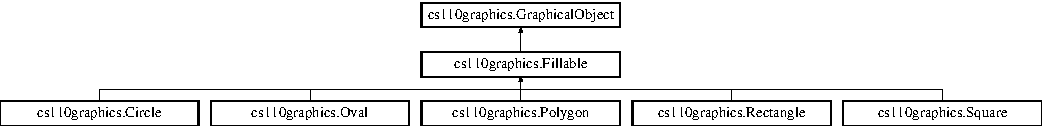
\includegraphics[height=1.68844cm]{classcs110graphics_1_1Fillable}
\end{center}
\end{figure}
\subsection*{Public Member Functions}
\begin{DoxyCompactItemize}
\item 
def \hyperlink{classcs110graphics_1_1Fillable_a6772d56158c9fe98a33f01d47cb8aa41}{get\_\-border\_\-color}
\begin{DoxyCompactList}\small\item\em Returns the border color. \item\end{DoxyCompactList}\item 
def \hyperlink{classcs110graphics_1_1Fillable_a6ed7a4288e84a090ec185c8bdff21d0f}{get\_\-border\_\-width}
\begin{DoxyCompactList}\small\item\em Returns the border width. \item\end{DoxyCompactList}\item 
def \hyperlink{classcs110graphics_1_1Fillable_a16c045bc9b63961b696914ee1a1d14d9}{get\_\-fill\_\-color}
\begin{DoxyCompactList}\small\item\em Returns fill color. \item\end{DoxyCompactList}\item 
def \hyperlink{classcs110graphics_1_1Fillable_a514fa0d21297c1372681afae9219fd58}{get\_\-pivot}
\begin{DoxyCompactList}\small\item\em Returns the pivot point. \item\end{DoxyCompactList}\item 
def \hyperlink{classcs110graphics_1_1Fillable_afa6710f6c314de39d19f06d9dd306d7d}{rotate}
\begin{DoxyCompactList}\small\item\em Rotates the object. \item\end{DoxyCompactList}\item 
def \hyperlink{classcs110graphics_1_1Fillable_a80d5b6b6d2ebae867dccecb803075749}{scale}
\begin{DoxyCompactList}\small\item\em Scales the object up or down depending on the factor. \item\end{DoxyCompactList}\item 
def \hyperlink{classcs110graphics_1_1Fillable_ae8f6c476e29c0810453dc16948e1730c}{move}
\begin{DoxyCompactList}\small\item\em Moves the object dx pixels horizontally and dy pixels vertically. \item\end{DoxyCompactList}\item 
def \hyperlink{classcs110graphics_1_1Fillable_adcabc14e76d1160ff591b9ef7f3d6a97}{move\_\-to}
\begin{DoxyCompactList}\small\item\em Moves a graphical object to a point. \item\end{DoxyCompactList}\item 
def \hyperlink{classcs110graphics_1_1Fillable_a2f830be5d970faac97759910d20d68a4}{set\_\-border\_\-color}
\begin{DoxyCompactList}\small\item\em Sets the border color. \item\end{DoxyCompactList}\item 
def \hyperlink{classcs110graphics_1_1Fillable_a09f05462cb2ed38fdccb244340f05b2b}{set\_\-border\_\-width}
\begin{DoxyCompactList}\small\item\em Sets the border width. \item\end{DoxyCompactList}\item 
def \hyperlink{classcs110graphics_1_1Fillable_a4f24c7186c8d057e42a0209eb1d56be7}{set\_\-fill\_\-color}
\begin{DoxyCompactList}\small\item\em Sets the fill color. \item\end{DoxyCompactList}\item 
def \hyperlink{classcs110graphics_1_1Fillable_a2a6066d1a11c0854ff5ee85e7d9ceb54}{set\_\-pivot}
\begin{DoxyCompactList}\small\item\em Sets the pivot point. \item\end{DoxyCompactList}\item 
def \hyperlink{classcs110graphics_1_1GraphicalObject_adb1af0d5a6baae3f9a08d21a3227c49f}{add\_\-handler}
\begin{DoxyCompactList}\small\item\em Adds a handler to the graphical object. \item\end{DoxyCompactList}\item 
def \hyperlink{classcs110graphics_1_1GraphicalObject_a062789c4cc9de38af32dcc4ff2058607}{get\_\-center}
\begin{DoxyCompactList}\small\item\em Returns the center of the object. \item\end{DoxyCompactList}\item 
def \hyperlink{classcs110graphics_1_1GraphicalObject_a6d9f5718cd0cf249e0d2842971bae17f}{get\_\-depth}
\begin{DoxyCompactList}\small\item\em Returns the depth of the object. \item\end{DoxyCompactList}\item 
def \hyperlink{classcs110graphics_1_1GraphicalObject_a20d76d4ee4419c3065d61deb6cbc6700}{set\_\-depth}
\begin{DoxyCompactList}\small\item\em Sets the depth of the \hyperlink{classcs110graphics_1_1GraphicalObject}{GraphicalObject}. \item\end{DoxyCompactList}\end{DoxyCompactItemize}


\subsection{Detailed Description}
This is a parent class of any object which can have its colors modified. No constructor exists in this class, but its methods are used by other objects that extend/inherit this class.

Default values:
\begin{DoxyItemize}
\item border color = \char`\"{}black\char`\"{}
\item border width = 2
\item fill color = \char`\"{}white\char`\"{}
\item pivot = center 
\end{DoxyItemize}

\subsection{Member Function Documentation}
\hypertarget{classcs110graphics_1_1GraphicalObject_adb1af0d5a6baae3f9a08d21a3227c49f}{
\index{cs110graphics::Fillable@{cs110graphics::Fillable}!add\_\-handler@{add\_\-handler}}
\index{add\_\-handler@{add\_\-handler}!cs110graphics::Fillable@{cs110graphics::Fillable}}
\subsubsection[{add\_\-handler}]{\setlength{\rightskip}{0pt plus 5cm}def cs110graphics.GraphicalObject.add\_\-handler ( {\em self}, \/   {\em handler\_\-object})\hspace{0.3cm}{\ttfamily  \mbox{[}inherited\mbox{]}}}}
\label{classcs110graphics_1_1GraphicalObject_adb1af0d5a6baae3f9a08d21a3227c49f}


Adds a handler to the graphical object. 
\begin{DoxyParams}{Parameters}
\item[{\em handler\_\-object}]-\/ \hyperlink{classcs110graphics_1_1EventHandler}{EventHandler} -\/ the object that handles the events for this \hyperlink{classcs110graphics_1_1GraphicalObject}{GraphicalObject} \end{DoxyParams}
\hypertarget{classcs110graphics_1_1Fillable_a6772d56158c9fe98a33f01d47cb8aa41}{
\index{cs110graphics::Fillable@{cs110graphics::Fillable}!get\_\-border\_\-color@{get\_\-border\_\-color}}
\index{get\_\-border\_\-color@{get\_\-border\_\-color}!cs110graphics::Fillable@{cs110graphics::Fillable}}
\subsubsection[{get\_\-border\_\-color}]{\setlength{\rightskip}{0pt plus 5cm}def cs110graphics.Fillable.get\_\-border\_\-color ( {\em self})}}
\label{classcs110graphics_1_1Fillable_a6772d56158c9fe98a33f01d47cb8aa41}


Returns the border color. \begin{DoxyReturn}{Returns}
border\_\-color -\/ str -\/ Can be either the name of a color (\char`\"{}yellow\char`\"{}), or a hex code (\char`\"{}\#FFFF00\char`\"{}) 
\end{DoxyReturn}
\hypertarget{classcs110graphics_1_1Fillable_a6ed7a4288e84a090ec185c8bdff21d0f}{
\index{cs110graphics::Fillable@{cs110graphics::Fillable}!get\_\-border\_\-width@{get\_\-border\_\-width}}
\index{get\_\-border\_\-width@{get\_\-border\_\-width}!cs110graphics::Fillable@{cs110graphics::Fillable}}
\subsubsection[{get\_\-border\_\-width}]{\setlength{\rightskip}{0pt plus 5cm}def cs110graphics.Fillable.get\_\-border\_\-width ( {\em self})}}
\label{classcs110graphics_1_1Fillable_a6ed7a4288e84a090ec185c8bdff21d0f}


Returns the border width. \begin{DoxyReturn}{Returns}
border\_\-width -\/ int 
\end{DoxyReturn}
\hypertarget{classcs110graphics_1_1GraphicalObject_a062789c4cc9de38af32dcc4ff2058607}{
\index{cs110graphics::Fillable@{cs110graphics::Fillable}!get\_\-center@{get\_\-center}}
\index{get\_\-center@{get\_\-center}!cs110graphics::Fillable@{cs110graphics::Fillable}}
\subsubsection[{get\_\-center}]{\setlength{\rightskip}{0pt plus 5cm}def cs110graphics.GraphicalObject.get\_\-center ( {\em self})\hspace{0.3cm}{\ttfamily  \mbox{[}inherited\mbox{]}}}}
\label{classcs110graphics_1_1GraphicalObject_a062789c4cc9de38af32dcc4ff2058607}


Returns the center of the object. \begin{DoxyReturn}{Returns}
center -\/ tuple 
\end{DoxyReturn}
\hypertarget{classcs110graphics_1_1GraphicalObject_a6d9f5718cd0cf249e0d2842971bae17f}{
\index{cs110graphics::Fillable@{cs110graphics::Fillable}!get\_\-depth@{get\_\-depth}}
\index{get\_\-depth@{get\_\-depth}!cs110graphics::Fillable@{cs110graphics::Fillable}}
\subsubsection[{get\_\-depth}]{\setlength{\rightskip}{0pt plus 5cm}def cs110graphics.GraphicalObject.get\_\-depth ( {\em self})\hspace{0.3cm}{\ttfamily  \mbox{[}inherited\mbox{]}}}}
\label{classcs110graphics_1_1GraphicalObject_a6d9f5718cd0cf249e0d2842971bae17f}


Returns the depth of the object. \begin{DoxyReturn}{Returns}
depth -\/ int 
\end{DoxyReturn}
\hypertarget{classcs110graphics_1_1Fillable_a16c045bc9b63961b696914ee1a1d14d9}{
\index{cs110graphics::Fillable@{cs110graphics::Fillable}!get\_\-fill\_\-color@{get\_\-fill\_\-color}}
\index{get\_\-fill\_\-color@{get\_\-fill\_\-color}!cs110graphics::Fillable@{cs110graphics::Fillable}}
\subsubsection[{get\_\-fill\_\-color}]{\setlength{\rightskip}{0pt plus 5cm}def cs110graphics.Fillable.get\_\-fill\_\-color ( {\em self})}}
\label{classcs110graphics_1_1Fillable_a16c045bc9b63961b696914ee1a1d14d9}


Returns fill color. \begin{DoxyReturn}{Returns}
color -\/ int -\/ Can be either the name of a color (\char`\"{}yellow\char`\"{}), or a hex code (\char`\"{}\#FFFF00\char`\"{}) 
\end{DoxyReturn}
\hypertarget{classcs110graphics_1_1Fillable_a514fa0d21297c1372681afae9219fd58}{
\index{cs110graphics::Fillable@{cs110graphics::Fillable}!get\_\-pivot@{get\_\-pivot}}
\index{get\_\-pivot@{get\_\-pivot}!cs110graphics::Fillable@{cs110graphics::Fillable}}
\subsubsection[{get\_\-pivot}]{\setlength{\rightskip}{0pt plus 5cm}def cs110graphics.Fillable.get\_\-pivot ( {\em self})}}
\label{classcs110graphics_1_1Fillable_a514fa0d21297c1372681afae9219fd58}


Returns the pivot point. \begin{DoxyReturn}{Returns}
pivot -\/ tuple (int $\ast$ int) 
\end{DoxyReturn}
\hypertarget{classcs110graphics_1_1Fillable_ae8f6c476e29c0810453dc16948e1730c}{
\index{cs110graphics::Fillable@{cs110graphics::Fillable}!move@{move}}
\index{move@{move}!cs110graphics::Fillable@{cs110graphics::Fillable}}
\subsubsection[{move}]{\setlength{\rightskip}{0pt plus 5cm}def cs110graphics.Fillable.move ( {\em self}, \/   {\em dx}, \/   {\em dy})}}
\label{classcs110graphics_1_1Fillable_ae8f6c476e29c0810453dc16948e1730c}


Moves the object dx pixels horizontally and dy pixels vertically. 
\begin{DoxyParams}{Parameters}
\item[{\em dx}]-\/ int \item[{\em dy}]-\/ int \end{DoxyParams}


Reimplemented from \hyperlink{classcs110graphics_1_1GraphicalObject_aa64d270fb83efa4a54e1a7953512f9cd}{cs110graphics.GraphicalObject}.\hypertarget{classcs110graphics_1_1Fillable_adcabc14e76d1160ff591b9ef7f3d6a97}{
\index{cs110graphics::Fillable@{cs110graphics::Fillable}!move\_\-to@{move\_\-to}}
\index{move\_\-to@{move\_\-to}!cs110graphics::Fillable@{cs110graphics::Fillable}}
\subsubsection[{move\_\-to}]{\setlength{\rightskip}{0pt plus 5cm}def cs110graphics.Fillable.move\_\-to ( {\em self}, \/   {\em point})}}
\label{classcs110graphics_1_1Fillable_adcabc14e76d1160ff591b9ef7f3d6a97}


Moves a graphical object to a point. 
\begin{DoxyParams}{Parameters}
\item[{\em point}]-\/ tuple of (int $\ast$ int) \end{DoxyParams}


Reimplemented from \hyperlink{classcs110graphics_1_1GraphicalObject_abe2d480265df7ac9447205c52c6946df}{cs110graphics.GraphicalObject}.\hypertarget{classcs110graphics_1_1Fillable_afa6710f6c314de39d19f06d9dd306d7d}{
\index{cs110graphics::Fillable@{cs110graphics::Fillable}!rotate@{rotate}}
\index{rotate@{rotate}!cs110graphics::Fillable@{cs110graphics::Fillable}}
\subsubsection[{rotate}]{\setlength{\rightskip}{0pt plus 5cm}def cs110graphics.Fillable.rotate ( {\em self}, \/   {\em degrees})}}
\label{classcs110graphics_1_1Fillable_afa6710f6c314de39d19f06d9dd306d7d}


Rotates the object. 
\begin{DoxyParams}{Parameters}
\item[{\em degrees}]-\/ int \end{DoxyParams}
\hypertarget{classcs110graphics_1_1Fillable_a80d5b6b6d2ebae867dccecb803075749}{
\index{cs110graphics::Fillable@{cs110graphics::Fillable}!scale@{scale}}
\index{scale@{scale}!cs110graphics::Fillable@{cs110graphics::Fillable}}
\subsubsection[{scale}]{\setlength{\rightskip}{0pt plus 5cm}def cs110graphics.Fillable.scale ( {\em self}, \/   {\em factor})}}
\label{classcs110graphics_1_1Fillable_a80d5b6b6d2ebae867dccecb803075749}


Scales the object up or down depending on the factor. 
\begin{DoxyParams}{Parameters}
\item[{\em factor}]-\/ float \end{DoxyParams}
\hypertarget{classcs110graphics_1_1Fillable_a2f830be5d970faac97759910d20d68a4}{
\index{cs110graphics::Fillable@{cs110graphics::Fillable}!set\_\-border\_\-color@{set\_\-border\_\-color}}
\index{set\_\-border\_\-color@{set\_\-border\_\-color}!cs110graphics::Fillable@{cs110graphics::Fillable}}
\subsubsection[{set\_\-border\_\-color}]{\setlength{\rightskip}{0pt plus 5cm}def cs110graphics.Fillable.set\_\-border\_\-color ( {\em self}, \/   {\em color})}}
\label{classcs110graphics_1_1Fillable_a2f830be5d970faac97759910d20d68a4}


Sets the border color. 
\begin{DoxyParams}{Parameters}
\item[{\em color}]-\/ string -\/ Can be either the name of a color (\char`\"{}yellow\char`\"{}), or a hex code (\char`\"{}\#FFFF00\char`\"{}) \end{DoxyParams}
\hypertarget{classcs110graphics_1_1Fillable_a09f05462cb2ed38fdccb244340f05b2b}{
\index{cs110graphics::Fillable@{cs110graphics::Fillable}!set\_\-border\_\-width@{set\_\-border\_\-width}}
\index{set\_\-border\_\-width@{set\_\-border\_\-width}!cs110graphics::Fillable@{cs110graphics::Fillable}}
\subsubsection[{set\_\-border\_\-width}]{\setlength{\rightskip}{0pt plus 5cm}def cs110graphics.Fillable.set\_\-border\_\-width ( {\em self}, \/   {\em width})}}
\label{classcs110graphics_1_1Fillable_a09f05462cb2ed38fdccb244340f05b2b}


Sets the border width. 
\begin{DoxyParams}{Parameters}
\item[{\em width}]-\/ int \end{DoxyParams}
\hypertarget{classcs110graphics_1_1GraphicalObject_a20d76d4ee4419c3065d61deb6cbc6700}{
\index{cs110graphics::Fillable@{cs110graphics::Fillable}!set\_\-depth@{set\_\-depth}}
\index{set\_\-depth@{set\_\-depth}!cs110graphics::Fillable@{cs110graphics::Fillable}}
\subsubsection[{set\_\-depth}]{\setlength{\rightskip}{0pt plus 5cm}def cs110graphics.GraphicalObject.set\_\-depth ( {\em self}, \/   {\em depth})\hspace{0.3cm}{\ttfamily  \mbox{[}inherited\mbox{]}}}}
\label{classcs110graphics_1_1GraphicalObject_a20d76d4ee4419c3065d61deb6cbc6700}


Sets the depth of the \hyperlink{classcs110graphics_1_1GraphicalObject}{GraphicalObject}. 
\begin{DoxyParams}{Parameters}
\item[{\em depth}]-\/ int \end{DoxyParams}
\hypertarget{classcs110graphics_1_1Fillable_a4f24c7186c8d057e42a0209eb1d56be7}{
\index{cs110graphics::Fillable@{cs110graphics::Fillable}!set\_\-fill\_\-color@{set\_\-fill\_\-color}}
\index{set\_\-fill\_\-color@{set\_\-fill\_\-color}!cs110graphics::Fillable@{cs110graphics::Fillable}}
\subsubsection[{set\_\-fill\_\-color}]{\setlength{\rightskip}{0pt plus 5cm}def cs110graphics.Fillable.set\_\-fill\_\-color ( {\em self}, \/   {\em color})}}
\label{classcs110graphics_1_1Fillable_a4f24c7186c8d057e42a0209eb1d56be7}


Sets the fill color. 
\begin{DoxyParams}{Parameters}
\item[{\em color}]-\/ string -\/ Can be either the name of a color (\char`\"{}yellow\char`\"{}), or a hex code (\char`\"{}\#FFFF00\char`\"{}) \end{DoxyParams}
\hypertarget{classcs110graphics_1_1Fillable_a2a6066d1a11c0854ff5ee85e7d9ceb54}{
\index{cs110graphics::Fillable@{cs110graphics::Fillable}!set\_\-pivot@{set\_\-pivot}}
\index{set\_\-pivot@{set\_\-pivot}!cs110graphics::Fillable@{cs110graphics::Fillable}}
\subsubsection[{set\_\-pivot}]{\setlength{\rightskip}{0pt plus 5cm}def cs110graphics.Fillable.set\_\-pivot ( {\em self}, \/   {\em pivot})}}
\label{classcs110graphics_1_1Fillable_a2a6066d1a11c0854ff5ee85e7d9ceb54}


Sets the pivot point. 
\begin{DoxyParams}{Parameters}
\item[{\em pivot}]-\/ tuple of (int $\ast$ int) \end{DoxyParams}


The documentation for this class was generated from the following file:\begin{DoxyCompactItemize}
\item 
\hyperlink{cs110graphics_8py}{cs110graphics.py}\end{DoxyCompactItemize}

\hypertarget{classcs110graphics_1_1GraphicalObject}{
\section{cs110graphics.GraphicalObject Class Reference}
\label{classcs110graphics_1_1GraphicalObject}\index{cs110graphics::GraphicalObject@{cs110graphics::GraphicalObject}}
}


This is a parent class of any object which can be put into \hyperlink{classcs110graphics_1_1Window}{Window}.  
Inheritance diagram for cs110graphics.GraphicalObject::\begin{figure}[H]
\begin{center}
\leavevmode
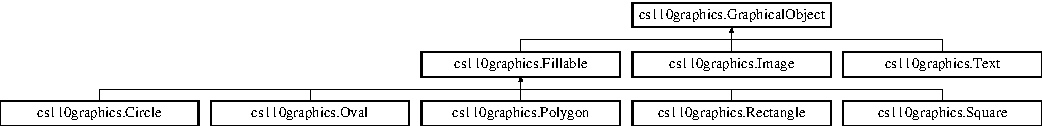
\includegraphics[height=1.68844cm]{classcs110graphics_1_1GraphicalObject}
\end{center}
\end{figure}
\subsection*{Public Member Functions}
\begin{DoxyCompactItemize}
\item 
def \hyperlink{classcs110graphics_1_1GraphicalObject_adb1af0d5a6baae3f9a08d21a3227c49f}{add\_\-handler}
\begin{DoxyCompactList}\small\item\em Adds a handler to the graphical object. \item\end{DoxyCompactList}\item 
def \hyperlink{classcs110graphics_1_1GraphicalObject_a062789c4cc9de38af32dcc4ff2058607}{get\_\-center}
\begin{DoxyCompactList}\small\item\em Returns the center of the object. \item\end{DoxyCompactList}\item 
def \hyperlink{classcs110graphics_1_1GraphicalObject_a6d9f5718cd0cf249e0d2842971bae17f}{get\_\-depth}
\begin{DoxyCompactList}\small\item\em Returns the depth of the object. \item\end{DoxyCompactList}\item 
def \hyperlink{classcs110graphics_1_1GraphicalObject_aa64d270fb83efa4a54e1a7953512f9cd}{move}
\begin{DoxyCompactList}\small\item\em Moves the object dx pixels horizontally and dy pixels vertically. \item\end{DoxyCompactList}\item 
def \hyperlink{classcs110graphics_1_1GraphicalObject_abe2d480265df7ac9447205c52c6946df}{move\_\-to}
\begin{DoxyCompactList}\small\item\em Moves a graphical object to a point. \item\end{DoxyCompactList}\item 
def \hyperlink{classcs110graphics_1_1GraphicalObject_a20d76d4ee4419c3065d61deb6cbc6700}{set\_\-depth}
\begin{DoxyCompactList}\small\item\em Sets the depth of the \hyperlink{classcs110graphics_1_1GraphicalObject}{GraphicalObject}. \item\end{DoxyCompactList}\end{DoxyCompactItemize}


\subsection{Detailed Description}
This is a parent class of any object which can be put into \hyperlink{classcs110graphics_1_1Window}{Window}. No constructor exists in this class, but its methods are used by other objects that extend/inherit this class.

Default values:
\begin{DoxyItemize}
\item depth = 50
\item center = (200, 200) 
\end{DoxyItemize}

\subsection{Member Function Documentation}
\hypertarget{classcs110graphics_1_1GraphicalObject_adb1af0d5a6baae3f9a08d21a3227c49f}{
\index{cs110graphics::GraphicalObject@{cs110graphics::GraphicalObject}!add\_\-handler@{add\_\-handler}}
\index{add\_\-handler@{add\_\-handler}!cs110graphics::GraphicalObject@{cs110graphics::GraphicalObject}}
\subsubsection[{add\_\-handler}]{\setlength{\rightskip}{0pt plus 5cm}def cs110graphics.GraphicalObject.add\_\-handler ( {\em self}, \/   {\em handler\_\-object})}}
\label{classcs110graphics_1_1GraphicalObject_adb1af0d5a6baae3f9a08d21a3227c49f}


Adds a handler to the graphical object. 
\begin{DoxyParams}{Parameters}
\item[{\em handler\_\-object}]-\/ \hyperlink{classcs110graphics_1_1EventHandler}{EventHandler} -\/ the object that handles the events for this \hyperlink{classcs110graphics_1_1GraphicalObject}{GraphicalObject} \end{DoxyParams}
\hypertarget{classcs110graphics_1_1GraphicalObject_a062789c4cc9de38af32dcc4ff2058607}{
\index{cs110graphics::GraphicalObject@{cs110graphics::GraphicalObject}!get\_\-center@{get\_\-center}}
\index{get\_\-center@{get\_\-center}!cs110graphics::GraphicalObject@{cs110graphics::GraphicalObject}}
\subsubsection[{get\_\-center}]{\setlength{\rightskip}{0pt plus 5cm}def cs110graphics.GraphicalObject.get\_\-center ( {\em self})}}
\label{classcs110graphics_1_1GraphicalObject_a062789c4cc9de38af32dcc4ff2058607}


Returns the center of the object. \begin{DoxyReturn}{Returns}
center -\/ tuple 
\end{DoxyReturn}
\hypertarget{classcs110graphics_1_1GraphicalObject_a6d9f5718cd0cf249e0d2842971bae17f}{
\index{cs110graphics::GraphicalObject@{cs110graphics::GraphicalObject}!get\_\-depth@{get\_\-depth}}
\index{get\_\-depth@{get\_\-depth}!cs110graphics::GraphicalObject@{cs110graphics::GraphicalObject}}
\subsubsection[{get\_\-depth}]{\setlength{\rightskip}{0pt plus 5cm}def cs110graphics.GraphicalObject.get\_\-depth ( {\em self})}}
\label{classcs110graphics_1_1GraphicalObject_a6d9f5718cd0cf249e0d2842971bae17f}


Returns the depth of the object. \begin{DoxyReturn}{Returns}
depth -\/ int 
\end{DoxyReturn}
\hypertarget{classcs110graphics_1_1GraphicalObject_aa64d270fb83efa4a54e1a7953512f9cd}{
\index{cs110graphics::GraphicalObject@{cs110graphics::GraphicalObject}!move@{move}}
\index{move@{move}!cs110graphics::GraphicalObject@{cs110graphics::GraphicalObject}}
\subsubsection[{move}]{\setlength{\rightskip}{0pt plus 5cm}def cs110graphics.GraphicalObject.move ( {\em self}, \/   {\em dx}, \/   {\em dy})}}
\label{classcs110graphics_1_1GraphicalObject_aa64d270fb83efa4a54e1a7953512f9cd}


Moves the object dx pixels horizontally and dy pixels vertically. 
\begin{DoxyParams}{Parameters}
\item[{\em dx}]-\/ int \item[{\em dy}]-\/ int \end{DoxyParams}


Reimplemented in \hyperlink{classcs110graphics_1_1Fillable_ae8f6c476e29c0810453dc16948e1730c}{cs110graphics.Fillable}, \hyperlink{classcs110graphics_1_1Image_a540d48247976343a91c610009a9af8cd}{cs110graphics.Image}, and \hyperlink{classcs110graphics_1_1Text_a6bd6f174fc82f2225a4d162ca6b90ec2}{cs110graphics.Text}.\hypertarget{classcs110graphics_1_1GraphicalObject_abe2d480265df7ac9447205c52c6946df}{
\index{cs110graphics::GraphicalObject@{cs110graphics::GraphicalObject}!move\_\-to@{move\_\-to}}
\index{move\_\-to@{move\_\-to}!cs110graphics::GraphicalObject@{cs110graphics::GraphicalObject}}
\subsubsection[{move\_\-to}]{\setlength{\rightskip}{0pt plus 5cm}def cs110graphics.GraphicalObject.move\_\-to ( {\em self}, \/   {\em point})}}
\label{classcs110graphics_1_1GraphicalObject_abe2d480265df7ac9447205c52c6946df}


Moves a graphical object to a point. 
\begin{DoxyParams}{Parameters}
\item[{\em point}]-\/ tuple of (int $\ast$ int) \end{DoxyParams}


Reimplemented in \hyperlink{classcs110graphics_1_1Fillable_adcabc14e76d1160ff591b9ef7f3d6a97}{cs110graphics.Fillable}, \hyperlink{classcs110graphics_1_1Image_a4b2e775fbb0cb523f6bc09028dc05c65}{cs110graphics.Image}, and \hyperlink{classcs110graphics_1_1Text_a615a76c8d2edd6c6af5d39d4e2577a27}{cs110graphics.Text}.\hypertarget{classcs110graphics_1_1GraphicalObject_a20d76d4ee4419c3065d61deb6cbc6700}{
\index{cs110graphics::GraphicalObject@{cs110graphics::GraphicalObject}!set\_\-depth@{set\_\-depth}}
\index{set\_\-depth@{set\_\-depth}!cs110graphics::GraphicalObject@{cs110graphics::GraphicalObject}}
\subsubsection[{set\_\-depth}]{\setlength{\rightskip}{0pt plus 5cm}def cs110graphics.GraphicalObject.set\_\-depth ( {\em self}, \/   {\em depth})}}
\label{classcs110graphics_1_1GraphicalObject_a20d76d4ee4419c3065d61deb6cbc6700}


Sets the depth of the \hyperlink{classcs110graphics_1_1GraphicalObject}{GraphicalObject}. 
\begin{DoxyParams}{Parameters}
\item[{\em depth}]-\/ int \end{DoxyParams}


The documentation for this class was generated from the following file:\begin{DoxyCompactItemize}
\item 
\hyperlink{cs110graphics_8py}{cs110graphics.py}\end{DoxyCompactItemize}

\hypertarget{classtext__move_1_1H2}{
\section{text\_\-move.H2 Class Reference}
\label{classtext__move_1_1H2}\index{text\_\-move::H2@{text\_\-move::H2}}
}
Inheritance diagram for text\_\-move.H2::\begin{figure}[H]
\begin{center}
\leavevmode
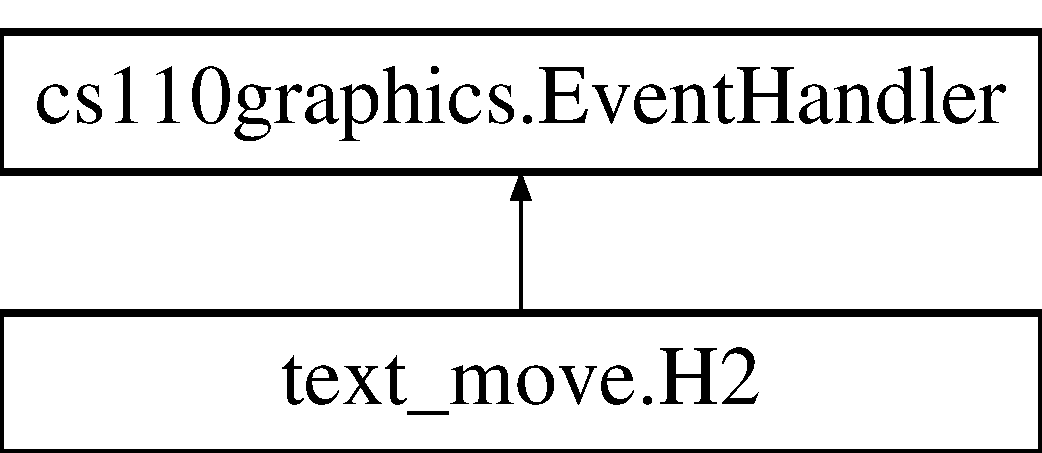
\includegraphics[height=2cm]{classtext__move_1_1H2}
\end{center}
\end{figure}
\subsection*{Public Member Functions}
\begin{DoxyCompactItemize}
\item 
def \hyperlink{classtext__move_1_1H2_a13611a7fe23eefc92b40ff3874e026bd}{handle\_\-mouse\_\-press}
\begin{DoxyCompactList}\small\item\em Handles a mouse press. \item\end{DoxyCompactList}\item 
def \hyperlink{classcs110graphics_1_1EventHandler_af3fb3531d0b23f1430a830586cd07906}{handle\_\-key\_\-press}
\begin{DoxyCompactList}\small\item\em Handles a key press. \item\end{DoxyCompactList}\item 
def \hyperlink{classcs110graphics_1_1EventHandler_a2849f60251baa44252992162521f2473}{handle\_\-key\_\-release}
\begin{DoxyCompactList}\small\item\em Handles a key release. \item\end{DoxyCompactList}\item 
def \hyperlink{classcs110graphics_1_1EventHandler_a13af3268f8a1aa36b8483eb2deffef15}{handle\_\-mouse\_\-enter}
\begin{DoxyCompactList}\small\item\em Handles when a mouse enters an object. \item\end{DoxyCompactList}\item 
def \hyperlink{classcs110graphics_1_1EventHandler_a5deaf2b6b8055e97ac0ddf6603132c64}{handle\_\-mouse\_\-leave}
\begin{DoxyCompactList}\small\item\em Handles when a mouse leaves an object. \item\end{DoxyCompactList}\item 
def \hyperlink{classcs110graphics_1_1EventHandler_a521fdcd170d15c0b8baa124c78b6d1ef}{handle\_\-mouse\_\-move}
\begin{DoxyCompactList}\small\item\em Handles a mouse move. \item\end{DoxyCompactList}\item 
def \hyperlink{classcs110graphics_1_1EventHandler_a320a7dbf68d37e0101b237bff1713088}{handle\_\-mouse\_\-release}
\begin{DoxyCompactList}\small\item\em Handles a mouse release. \item\end{DoxyCompactList}\end{DoxyCompactItemize}


\subsection{Member Function Documentation}
\hypertarget{classcs110graphics_1_1EventHandler_af3fb3531d0b23f1430a830586cd07906}{
\index{text\_\-move::H2@{text\_\-move::H2}!handle\_\-key\_\-press@{handle\_\-key\_\-press}}
\index{handle\_\-key\_\-press@{handle\_\-key\_\-press}!text_move::H2@{text\_\-move::H2}}
\subsubsection[{handle\_\-key\_\-press}]{\setlength{\rightskip}{0pt plus 5cm}def cs110graphics.EventHandler.handle\_\-key\_\-press ( {\em self}, \/   {\em event})\hspace{0.3cm}{\ttfamily  \mbox{[}inherited\mbox{]}}}}
\label{classcs110graphics_1_1EventHandler_af3fb3531d0b23f1430a830586cd07906}


Handles a key press. This function will be called whenever a key is pressed while the window is active. The event parameter can be used to determine which key was pressed. For example: 
\begin{DoxyCode}
 class Handler(EventHandler):
     def handle_key_press(self, event):
         if "a" == event.get_key():
             # do something when a is pressed...
         else:
             # do something else...
\end{DoxyCode}
 
\begin{DoxyParams}{Parameters}
\item[{\em event}]-\/ \hyperlink{classcs110graphics_1_1Event}{Event} -\/ the event that occurred \end{DoxyParams}


Reimplemented in \hyperlink{classtest_1_1Handler_a3d418670cfafce344b8b7155b4df438e}{test.Handler}, \hyperlink{classtest_1_1Bot_a23b90152ec8fa124851cd5fe6944beed}{test.Bot}, and \hyperlink{classtext__move_1_1Handler_a5a42b4eb6df32fce14be58a45a7a82f0}{text\_\-move.Handler}.\hypertarget{classcs110graphics_1_1EventHandler_a2849f60251baa44252992162521f2473}{
\index{text\_\-move::H2@{text\_\-move::H2}!handle\_\-key\_\-release@{handle\_\-key\_\-release}}
\index{handle\_\-key\_\-release@{handle\_\-key\_\-release}!text_move::H2@{text\_\-move::H2}}
\subsubsection[{handle\_\-key\_\-release}]{\setlength{\rightskip}{0pt plus 5cm}def cs110graphics.EventHandler.handle\_\-key\_\-release ( {\em self}, \/   {\em event})\hspace{0.3cm}{\ttfamily  \mbox{[}inherited\mbox{]}}}}
\label{classcs110graphics_1_1EventHandler_a2849f60251baa44252992162521f2473}


Handles a key release. This method will be called whenever a key is released while the window is active. The event parameter can be used to determine which key was pressed. For example: 
\begin{DoxyCode}
 class Handler(EventHandler):
     def handle_key_release(self, event):
         if "a" == event.get_key():
             # do something when a is released...
         else:
             # do something else...
\end{DoxyCode}
 
\begin{DoxyParams}{Parameters}
\item[{\em event}]-\/ \hyperlink{classcs110graphics_1_1Event}{Event} -\/ the event that occurred \end{DoxyParams}


Reimplemented in \hyperlink{classtest_1_1Bot_a173d0fff530e0987193e9006b24f218b}{test.Bot}.\hypertarget{classcs110graphics_1_1EventHandler_a13af3268f8a1aa36b8483eb2deffef15}{
\index{text\_\-move::H2@{text\_\-move::H2}!handle\_\-mouse\_\-enter@{handle\_\-mouse\_\-enter}}
\index{handle\_\-mouse\_\-enter@{handle\_\-mouse\_\-enter}!text_move::H2@{text\_\-move::H2}}
\subsubsection[{handle\_\-mouse\_\-enter}]{\setlength{\rightskip}{0pt plus 5cm}def cs110graphics.EventHandler.handle\_\-mouse\_\-enter ( {\em self}, \/   {\em event})\hspace{0.3cm}{\ttfamily  \mbox{[}inherited\mbox{]}}}}
\label{classcs110graphics_1_1EventHandler_a13af3268f8a1aa36b8483eb2deffef15}


Handles when a mouse enters an object. \begin{Desc}
\item[\hyperlink{bug__bug000001}{Bug}]Overrides of this method is likely to be called more often than expected and many \hyperlink{classcs110graphics_1_1GraphicalObject}{GraphicalObject} methods will not work correctly with when called within the method, avoid using this if possible.\end{Desc}
This is called by the system when the mouse enters the \hyperlink{classcs110graphics_1_1GraphicalObject}{GraphicalObject} that this handler is an event handler for. The event parameter can be used to determine the location at which the mouse entered the object. 
\begin{DoxyCode}
 class Handler(EventHandler):
     def handle_mouse_enter(self, event):
         mouse_location = event.get_mouse_location()
\end{DoxyCode}
 
\begin{DoxyParams}{Parameters}
\item[{\em event}]-\/ \hyperlink{classcs110graphics_1_1Event}{Event} -\/ the event that occurred \end{DoxyParams}


Reimplemented in \hyperlink{classtest_1_1Bot_a0b184ab86d0dd6121e55394a24c8751e}{test.Bot}, and \hyperlink{classtext__move_1_1Handler_a51652a1d51554e661117de1ee7856169}{text\_\-move.Handler}.\hypertarget{classcs110graphics_1_1EventHandler_a5deaf2b6b8055e97ac0ddf6603132c64}{
\index{text\_\-move::H2@{text\_\-move::H2}!handle\_\-mouse\_\-leave@{handle\_\-mouse\_\-leave}}
\index{handle\_\-mouse\_\-leave@{handle\_\-mouse\_\-leave}!text_move::H2@{text\_\-move::H2}}
\subsubsection[{handle\_\-mouse\_\-leave}]{\setlength{\rightskip}{0pt plus 5cm}def cs110graphics.EventHandler.handle\_\-mouse\_\-leave ( {\em self}, \/   {\em event})\hspace{0.3cm}{\ttfamily  \mbox{[}inherited\mbox{]}}}}
\label{classcs110graphics_1_1EventHandler_a5deaf2b6b8055e97ac0ddf6603132c64}


Handles when a mouse leaves an object. This is called by the system when the mouse leaves the \hyperlink{classcs110graphics_1_1GraphicalObject}{GraphicalObject} that this handler is an event handler for. The event parameter can be used to determine the location at which the mouse left the object. 
\begin{DoxyCode}
 class Handler(EventHandler):
     def handle_mouse_leave(self, event):
         mouse_location = event.get_mouse_location()
\end{DoxyCode}
 
\begin{DoxyParams}{Parameters}
\item[{\em event}]-\/ \hyperlink{classcs110graphics_1_1Event}{Event} -\/ the event that occurred \end{DoxyParams}


Reimplemented in \hyperlink{classtest_1_1Bot_a2b65e6ecaba1afb4f117b74a684b4387}{test.Bot}.\hypertarget{classcs110graphics_1_1EventHandler_a521fdcd170d15c0b8baa124c78b6d1ef}{
\index{text\_\-move::H2@{text\_\-move::H2}!handle\_\-mouse\_\-move@{handle\_\-mouse\_\-move}}
\index{handle\_\-mouse\_\-move@{handle\_\-mouse\_\-move}!text_move::H2@{text\_\-move::H2}}
\subsubsection[{handle\_\-mouse\_\-move}]{\setlength{\rightskip}{0pt plus 5cm}def cs110graphics.EventHandler.handle\_\-mouse\_\-move ( {\em self}, \/   {\em event})\hspace{0.3cm}{\ttfamily  \mbox{[}inherited\mbox{]}}}}
\label{classcs110graphics_1_1EventHandler_a521fdcd170d15c0b8baa124c78b6d1ef}


Handles a mouse move. This is called by the system when the mouse moves within the \hyperlink{classcs110graphics_1_1GraphicalObject}{GraphicalObject} that this handler is an event handler for. The event parameter can be used to determine the location that the mouse moved to. 
\begin{DoxyCode}
 class Handler(EventHandler):
     def handle_mouse_move(self, event):
         mouse_location = event.get_mouse_location()
\end{DoxyCode}
 
\begin{DoxyParams}{Parameters}
\item[{\em event}]-\/ \hyperlink{classcs110graphics_1_1Event}{Event} -\/ the event that occurred \end{DoxyParams}


Reimplemented in \hyperlink{classtest_1_1Handler_a88a2d58962eb4bf7338332848fa5fc3a}{test.Handler}, and \hyperlink{classtest_1_1Bot_ad1464516fb04013fa7e353a78f0ec218}{test.Bot}.\hypertarget{classtext__move_1_1H2_a13611a7fe23eefc92b40ff3874e026bd}{
\index{text\_\-move::H2@{text\_\-move::H2}!handle\_\-mouse\_\-press@{handle\_\-mouse\_\-press}}
\index{handle\_\-mouse\_\-press@{handle\_\-mouse\_\-press}!text_move::H2@{text\_\-move::H2}}
\subsubsection[{handle\_\-mouse\_\-press}]{\setlength{\rightskip}{0pt plus 5cm}def text\_\-move.H2.handle\_\-mouse\_\-press ( {\em self}, \/   {\em event})}}
\label{classtext__move_1_1H2_a13611a7fe23eefc92b40ff3874e026bd}


Handles a mouse press. This is called by the system when a mouse button is pressed while the mouse is on the GraphicalObject that this handler is an event handler for. The event parameter can be used to determine the location at which the mouse button was pressed and which mouse button was pressed. 
\begin{DoxyCode}
 class Handler(EventHandler):
     def handle_mouse_press(self, event):
         mouse_location = event.get_mouse_location()
         mouse_button = event.get_button()
\end{DoxyCode}
 
\begin{DoxyParams}{Parameters}
\item[{\em event}]-\/ Event -\/ the event that occurred \end{DoxyParams}


Reimplemented from \hyperlink{classcs110graphics_1_1EventHandler_a547873123ebcd3fcc63a2e03d2a2fee3}{cs110graphics.EventHandler}.\hypertarget{classcs110graphics_1_1EventHandler_a320a7dbf68d37e0101b237bff1713088}{
\index{text\_\-move::H2@{text\_\-move::H2}!handle\_\-mouse\_\-release@{handle\_\-mouse\_\-release}}
\index{handle\_\-mouse\_\-release@{handle\_\-mouse\_\-release}!text_move::H2@{text\_\-move::H2}}
\subsubsection[{handle\_\-mouse\_\-release}]{\setlength{\rightskip}{0pt plus 5cm}def cs110graphics.EventHandler.handle\_\-mouse\_\-release ( {\em self}, \/   {\em event})\hspace{0.3cm}{\ttfamily  \mbox{[}inherited\mbox{]}}}}
\label{classcs110graphics_1_1EventHandler_a320a7dbf68d37e0101b237bff1713088}


Handles a mouse release. This is called by the system when a mouse button is released while the mouse is on the \hyperlink{classcs110graphics_1_1GraphicalObject}{GraphicalObject} that this handler is an event handler for. The event parameter can be used to determine the location at which the mouse button was released and which mouse button was released. 
\begin{DoxyCode}
 class Handler(EventHandler):
     def handle_mouse_release(self, event):
         mouse_location = event.get_mouse_location()
         mouse_button = event.get_button()
\end{DoxyCode}
 
\begin{DoxyParams}{Parameters}
\item[{\em event}]-\/ \hyperlink{classcs110graphics_1_1Event}{Event} -\/ the event that occurred \end{DoxyParams}


Reimplemented in \hyperlink{classsample_1_1Remover_a84484de500f08402e582c126432e0cf1}{sample.Remover}, and \hyperlink{classtest_1_1Bot_a18fc05b6e2c1e42e1b6c639f4844a059}{test.Bot}.

The documentation for this class was generated from the following file:\begin{DoxyCompactItemize}
\item 
text\_\-move.py\end{DoxyCompactItemize}

\hypertarget{classtext__move_1_1Handler}{
\section{text\_\-move.Handler Class Reference}
\label{classtext__move_1_1Handler}\index{text\_\-move::Handler@{text\_\-move::Handler}}
}
Inheritance diagram for text\_\-move.Handler::\begin{figure}[H]
\begin{center}
\leavevmode
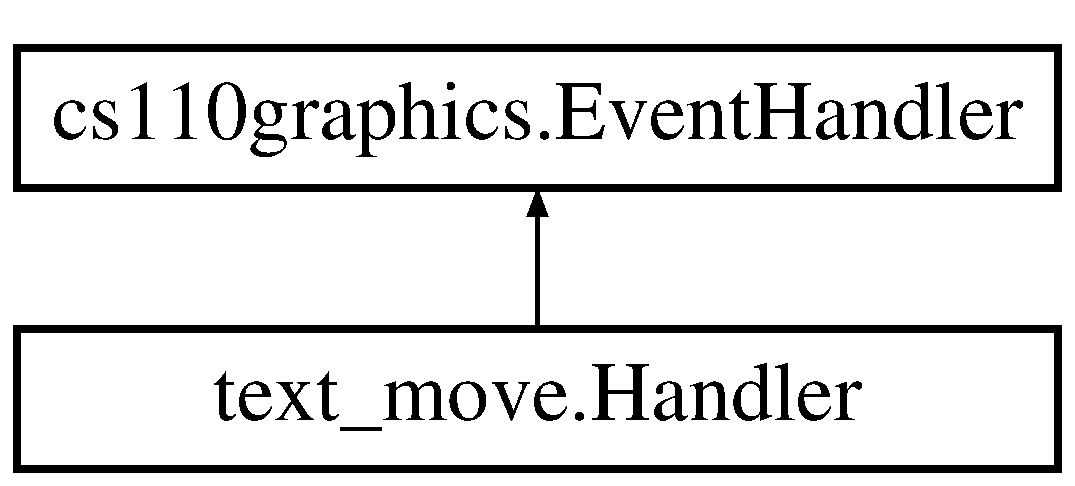
\includegraphics[height=2cm]{classtext__move_1_1Handler}
\end{center}
\end{figure}
\subsection*{Public Member Functions}
\begin{DoxyCompactItemize}
\item 
def \hyperlink{classtext__move_1_1Handler_a5a42b4eb6df32fce14be58a45a7a82f0}{handle\_\-key\_\-press}
\begin{DoxyCompactList}\small\item\em Handles a key press. \item\end{DoxyCompactList}\item 
def \hyperlink{classtext__move_1_1Handler_a51652a1d51554e661117de1ee7856169}{handle\_\-mouse\_\-enter}
\begin{DoxyCompactList}\small\item\em Handles when a mouse enters an object. \item\end{DoxyCompactList}\item 
def \hyperlink{classcs110graphics_1_1EventHandler_a2849f60251baa44252992162521f2473}{handle\_\-key\_\-release}
\begin{DoxyCompactList}\small\item\em Handles a key release. \item\end{DoxyCompactList}\item 
def \hyperlink{classcs110graphics_1_1EventHandler_a5deaf2b6b8055e97ac0ddf6603132c64}{handle\_\-mouse\_\-leave}
\begin{DoxyCompactList}\small\item\em Handles when a mouse leaves an object. \item\end{DoxyCompactList}\item 
def \hyperlink{classcs110graphics_1_1EventHandler_a521fdcd170d15c0b8baa124c78b6d1ef}{handle\_\-mouse\_\-move}
\begin{DoxyCompactList}\small\item\em Handles a mouse move. \item\end{DoxyCompactList}\item 
def \hyperlink{classcs110graphics_1_1EventHandler_a547873123ebcd3fcc63a2e03d2a2fee3}{handle\_\-mouse\_\-press}
\begin{DoxyCompactList}\small\item\em Handles a mouse press. \item\end{DoxyCompactList}\item 
def \hyperlink{classcs110graphics_1_1EventHandler_a320a7dbf68d37e0101b237bff1713088}{handle\_\-mouse\_\-release}
\begin{DoxyCompactList}\small\item\em Handles a mouse release. \item\end{DoxyCompactList}\end{DoxyCompactItemize}


\subsection{Member Function Documentation}
\hypertarget{classtext__move_1_1Handler_a5a42b4eb6df32fce14be58a45a7a82f0}{
\index{text\_\-move::Handler@{text\_\-move::Handler}!handle\_\-key\_\-press@{handle\_\-key\_\-press}}
\index{handle\_\-key\_\-press@{handle\_\-key\_\-press}!text_move::Handler@{text\_\-move::Handler}}
\subsubsection[{handle\_\-key\_\-press}]{\setlength{\rightskip}{0pt plus 5cm}def text\_\-move.Handler.handle\_\-key\_\-press ( {\em self}, \/   {\em event})}}
\label{classtext__move_1_1Handler_a5a42b4eb6df32fce14be58a45a7a82f0}


Handles a key press. This function will be called whenever a key is pressed while the window is active. The event parameter can be used to determine which key was pressed. For example: 
\begin{DoxyCode}
 class Handler(EventHandler):
     def handle_key_press(self, event):
         if "a" == event.get_key():
             # do something when a is pressed...
         else:
             # do something else...
\end{DoxyCode}
 
\begin{DoxyParams}{Parameters}
\item[{\em event}]-\/ Event -\/ the event that occurred \end{DoxyParams}


Reimplemented from \hyperlink{classcs110graphics_1_1EventHandler_af3fb3531d0b23f1430a830586cd07906}{cs110graphics.EventHandler}.\hypertarget{classcs110graphics_1_1EventHandler_a2849f60251baa44252992162521f2473}{
\index{text\_\-move::Handler@{text\_\-move::Handler}!handle\_\-key\_\-release@{handle\_\-key\_\-release}}
\index{handle\_\-key\_\-release@{handle\_\-key\_\-release}!text_move::Handler@{text\_\-move::Handler}}
\subsubsection[{handle\_\-key\_\-release}]{\setlength{\rightskip}{0pt plus 5cm}def cs110graphics.EventHandler.handle\_\-key\_\-release ( {\em self}, \/   {\em event})\hspace{0.3cm}{\ttfamily  \mbox{[}inherited\mbox{]}}}}
\label{classcs110graphics_1_1EventHandler_a2849f60251baa44252992162521f2473}


Handles a key release. This method will be called whenever a key is released while the window is active. The event parameter can be used to determine which key was pressed. For example: 
\begin{DoxyCode}
 class Handler(EventHandler):
     def handle_key_release(self, event):
         if "a" == event.get_key():
             # do something when a is released...
         else:
             # do something else...
\end{DoxyCode}
 
\begin{DoxyParams}{Parameters}
\item[{\em event}]-\/ \hyperlink{classcs110graphics_1_1Event}{Event} -\/ the event that occurred \end{DoxyParams}


Reimplemented in \hyperlink{classtest_1_1Bot_a173d0fff530e0987193e9006b24f218b}{test.Bot}.\hypertarget{classtext__move_1_1Handler_a51652a1d51554e661117de1ee7856169}{
\index{text\_\-move::Handler@{text\_\-move::Handler}!handle\_\-mouse\_\-enter@{handle\_\-mouse\_\-enter}}
\index{handle\_\-mouse\_\-enter@{handle\_\-mouse\_\-enter}!text_move::Handler@{text\_\-move::Handler}}
\subsubsection[{handle\_\-mouse\_\-enter}]{\setlength{\rightskip}{0pt plus 5cm}def text\_\-move.Handler.handle\_\-mouse\_\-enter ( {\em self}, \/   {\em event})}}
\label{classtext__move_1_1Handler_a51652a1d51554e661117de1ee7856169}


Handles when a mouse enters an object. \begin{Desc}
\item[\hyperlink{bug__bug000001}{Bug}]Overrides of this method is likely to be called more often than expected and many GraphicalObject methods will not work correctly with when called within the method, avoid using this if possible.\end{Desc}
This is called by the system when the mouse enters the GraphicalObject that this handler is an event handler for. The event parameter can be used to determine the location at which the mouse entered the object. 
\begin{DoxyCode}
 class Handler(EventHandler):
     def handle_mouse_enter(self, event):
         mouse_location = event.get_mouse_location()
\end{DoxyCode}
 
\begin{DoxyParams}{Parameters}
\item[{\em event}]-\/ Event -\/ the event that occurred \end{DoxyParams}


Reimplemented from \hyperlink{classcs110graphics_1_1EventHandler_a13af3268f8a1aa36b8483eb2deffef15}{cs110graphics.EventHandler}.\hypertarget{classcs110graphics_1_1EventHandler_a5deaf2b6b8055e97ac0ddf6603132c64}{
\index{text\_\-move::Handler@{text\_\-move::Handler}!handle\_\-mouse\_\-leave@{handle\_\-mouse\_\-leave}}
\index{handle\_\-mouse\_\-leave@{handle\_\-mouse\_\-leave}!text_move::Handler@{text\_\-move::Handler}}
\subsubsection[{handle\_\-mouse\_\-leave}]{\setlength{\rightskip}{0pt plus 5cm}def cs110graphics.EventHandler.handle\_\-mouse\_\-leave ( {\em self}, \/   {\em event})\hspace{0.3cm}{\ttfamily  \mbox{[}inherited\mbox{]}}}}
\label{classcs110graphics_1_1EventHandler_a5deaf2b6b8055e97ac0ddf6603132c64}


Handles when a mouse leaves an object. This is called by the system when the mouse leaves the \hyperlink{classcs110graphics_1_1GraphicalObject}{GraphicalObject} that this handler is an event handler for. The event parameter can be used to determine the location at which the mouse left the object. 
\begin{DoxyCode}
 class Handler(EventHandler):
     def handle_mouse_leave(self, event):
         mouse_location = event.get_mouse_location()
\end{DoxyCode}
 
\begin{DoxyParams}{Parameters}
\item[{\em event}]-\/ \hyperlink{classcs110graphics_1_1Event}{Event} -\/ the event that occurred \end{DoxyParams}


Reimplemented in \hyperlink{classtest_1_1Bot_a2b65e6ecaba1afb4f117b74a684b4387}{test.Bot}.\hypertarget{classcs110graphics_1_1EventHandler_a521fdcd170d15c0b8baa124c78b6d1ef}{
\index{text\_\-move::Handler@{text\_\-move::Handler}!handle\_\-mouse\_\-move@{handle\_\-mouse\_\-move}}
\index{handle\_\-mouse\_\-move@{handle\_\-mouse\_\-move}!text_move::Handler@{text\_\-move::Handler}}
\subsubsection[{handle\_\-mouse\_\-move}]{\setlength{\rightskip}{0pt plus 5cm}def cs110graphics.EventHandler.handle\_\-mouse\_\-move ( {\em self}, \/   {\em event})\hspace{0.3cm}{\ttfamily  \mbox{[}inherited\mbox{]}}}}
\label{classcs110graphics_1_1EventHandler_a521fdcd170d15c0b8baa124c78b6d1ef}


Handles a mouse move. This is called by the system when the mouse moves within the \hyperlink{classcs110graphics_1_1GraphicalObject}{GraphicalObject} that this handler is an event handler for. The event parameter can be used to determine the location that the mouse moved to. 
\begin{DoxyCode}
 class Handler(EventHandler):
     def handle_mouse_move(self, event):
         mouse_location = event.get_mouse_location()
\end{DoxyCode}
 
\begin{DoxyParams}{Parameters}
\item[{\em event}]-\/ \hyperlink{classcs110graphics_1_1Event}{Event} -\/ the event that occurred \end{DoxyParams}


Reimplemented in \hyperlink{classtest_1_1Handler_a88a2d58962eb4bf7338332848fa5fc3a}{test.Handler}, and \hyperlink{classtest_1_1Bot_ad1464516fb04013fa7e353a78f0ec218}{test.Bot}.\hypertarget{classcs110graphics_1_1EventHandler_a547873123ebcd3fcc63a2e03d2a2fee3}{
\index{text\_\-move::Handler@{text\_\-move::Handler}!handle\_\-mouse\_\-press@{handle\_\-mouse\_\-press}}
\index{handle\_\-mouse\_\-press@{handle\_\-mouse\_\-press}!text_move::Handler@{text\_\-move::Handler}}
\subsubsection[{handle\_\-mouse\_\-press}]{\setlength{\rightskip}{0pt plus 5cm}def cs110graphics.EventHandler.handle\_\-mouse\_\-press ( {\em self}, \/   {\em event})\hspace{0.3cm}{\ttfamily  \mbox{[}inherited\mbox{]}}}}
\label{classcs110graphics_1_1EventHandler_a547873123ebcd3fcc63a2e03d2a2fee3}


Handles a mouse press. This is called by the system when a mouse button is pressed while the mouse is on the \hyperlink{classcs110graphics_1_1GraphicalObject}{GraphicalObject} that this handler is an event handler for. The event parameter can be used to determine the location at which the mouse button was pressed and which mouse button was pressed. 
\begin{DoxyCode}
 class Handler(EventHandler):
     def handle_mouse_press(self, event):
         mouse_location = event.get_mouse_location()
         mouse_button = event.get_button()
\end{DoxyCode}
 
\begin{DoxyParams}{Parameters}
\item[{\em event}]-\/ \hyperlink{classcs110graphics_1_1Event}{Event} -\/ the event that occurred \end{DoxyParams}


Reimplemented in \hyperlink{classtest_1_1Bot_a970422a4391cc2b9ff89a2e42063bb6e}{test.Bot}, and \hyperlink{classtext__move_1_1H2_a13611a7fe23eefc92b40ff3874e026bd}{text\_\-move.H2}.\hypertarget{classcs110graphics_1_1EventHandler_a320a7dbf68d37e0101b237bff1713088}{
\index{text\_\-move::Handler@{text\_\-move::Handler}!handle\_\-mouse\_\-release@{handle\_\-mouse\_\-release}}
\index{handle\_\-mouse\_\-release@{handle\_\-mouse\_\-release}!text_move::Handler@{text\_\-move::Handler}}
\subsubsection[{handle\_\-mouse\_\-release}]{\setlength{\rightskip}{0pt plus 5cm}def cs110graphics.EventHandler.handle\_\-mouse\_\-release ( {\em self}, \/   {\em event})\hspace{0.3cm}{\ttfamily  \mbox{[}inherited\mbox{]}}}}
\label{classcs110graphics_1_1EventHandler_a320a7dbf68d37e0101b237bff1713088}


Handles a mouse release. This is called by the system when a mouse button is released while the mouse is on the \hyperlink{classcs110graphics_1_1GraphicalObject}{GraphicalObject} that this handler is an event handler for. The event parameter can be used to determine the location at which the mouse button was released and which mouse button was released. 
\begin{DoxyCode}
 class Handler(EventHandler):
     def handle_mouse_release(self, event):
         mouse_location = event.get_mouse_location()
         mouse_button = event.get_button()
\end{DoxyCode}
 
\begin{DoxyParams}{Parameters}
\item[{\em event}]-\/ \hyperlink{classcs110graphics_1_1Event}{Event} -\/ the event that occurred \end{DoxyParams}


Reimplemented in \hyperlink{classsample_1_1Remover_a84484de500f08402e582c126432e0cf1}{sample.Remover}, and \hyperlink{classtest_1_1Bot_a18fc05b6e2c1e42e1b6c639f4844a059}{test.Bot}.

The documentation for this class was generated from the following file:\begin{DoxyCompactItemize}
\item 
text\_\-move.py\end{DoxyCompactItemize}

\hypertarget{classtest_1_1Handler}{
\section{test.Handler Class Reference}
\label{classtest_1_1Handler}\index{test::Handler@{test::Handler}}
}
Inheritance diagram for test.Handler::\begin{figure}[H]
\begin{center}
\leavevmode
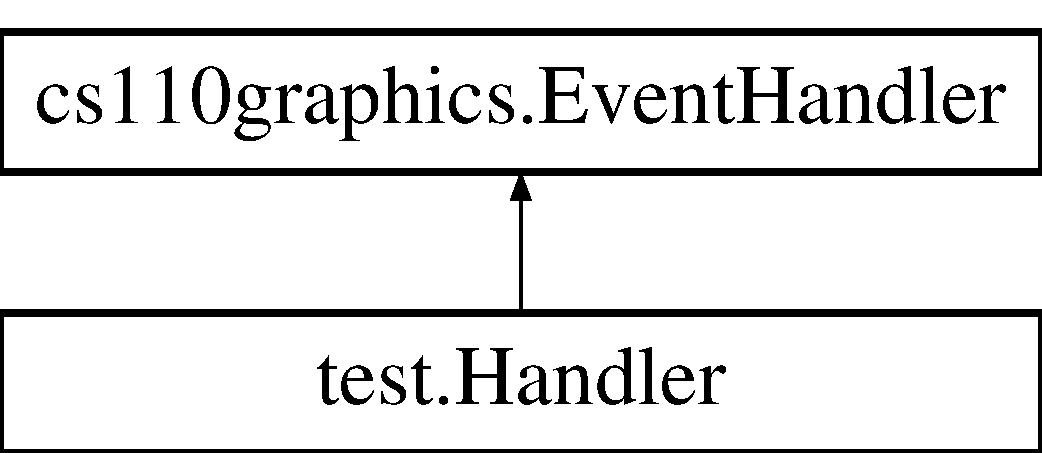
\includegraphics[height=2cm]{classtest_1_1Handler}
\end{center}
\end{figure}
\subsection*{Public Member Functions}
\begin{DoxyCompactItemize}
\item 
def \hyperlink{classtest_1_1Handler_a3d418670cfafce344b8b7155b4df438e}{handle\_\-key\_\-press}
\begin{DoxyCompactList}\small\item\em Handles a key press. \item\end{DoxyCompactList}\item 
def \hyperlink{classtest_1_1Handler_a88a2d58962eb4bf7338332848fa5fc3a}{handle\_\-mouse\_\-move}
\begin{DoxyCompactList}\small\item\em Handles a mouse move. \item\end{DoxyCompactList}\item 
def \hyperlink{classcs110graphics_1_1EventHandler_a2849f60251baa44252992162521f2473}{handle\_\-key\_\-release}
\begin{DoxyCompactList}\small\item\em Handles a key release. \item\end{DoxyCompactList}\item 
def \hyperlink{classcs110graphics_1_1EventHandler_a13af3268f8a1aa36b8483eb2deffef15}{handle\_\-mouse\_\-enter}
\begin{DoxyCompactList}\small\item\em Handles when a mouse enters an object. \item\end{DoxyCompactList}\item 
def \hyperlink{classcs110graphics_1_1EventHandler_a5deaf2b6b8055e97ac0ddf6603132c64}{handle\_\-mouse\_\-leave}
\begin{DoxyCompactList}\small\item\em Handles when a mouse leaves an object. \item\end{DoxyCompactList}\item 
def \hyperlink{classcs110graphics_1_1EventHandler_a547873123ebcd3fcc63a2e03d2a2fee3}{handle\_\-mouse\_\-press}
\begin{DoxyCompactList}\small\item\em Handles a mouse press. \item\end{DoxyCompactList}\item 
def \hyperlink{classcs110graphics_1_1EventHandler_a320a7dbf68d37e0101b237bff1713088}{handle\_\-mouse\_\-release}
\begin{DoxyCompactList}\small\item\em Handles a mouse release. \item\end{DoxyCompactList}\end{DoxyCompactItemize}


\subsection{Member Function Documentation}
\hypertarget{classtest_1_1Handler_a3d418670cfafce344b8b7155b4df438e}{
\index{test::Handler@{test::Handler}!handle\_\-key\_\-press@{handle\_\-key\_\-press}}
\index{handle\_\-key\_\-press@{handle\_\-key\_\-press}!test::Handler@{test::Handler}}
\subsubsection[{handle\_\-key\_\-press}]{\setlength{\rightskip}{0pt plus 5cm}def test.Handler.handle\_\-key\_\-press ( {\em self}, \/   {\em event})}}
\label{classtest_1_1Handler_a3d418670cfafce344b8b7155b4df438e}


Handles a key press. This function will be called whenever a key is pressed while the window is active. The event parameter can be used to determine which key was pressed. For example: 
\begin{DoxyCode}
 class Handler(EventHandler):
     def handle_key_press(self, event):
         if "a" == event.get_key():
             # do something when a is pressed...
         else:
             # do something else...
\end{DoxyCode}
 
\begin{DoxyParams}{Parameters}
\item[{\em event}]-\/ Event -\/ the event that occurred \end{DoxyParams}


Reimplemented from \hyperlink{classcs110graphics_1_1EventHandler_af3fb3531d0b23f1430a830586cd07906}{cs110graphics.EventHandler}.\hypertarget{classcs110graphics_1_1EventHandler_a2849f60251baa44252992162521f2473}{
\index{test::Handler@{test::Handler}!handle\_\-key\_\-release@{handle\_\-key\_\-release}}
\index{handle\_\-key\_\-release@{handle\_\-key\_\-release}!test::Handler@{test::Handler}}
\subsubsection[{handle\_\-key\_\-release}]{\setlength{\rightskip}{0pt plus 5cm}def cs110graphics.EventHandler.handle\_\-key\_\-release ( {\em self}, \/   {\em event})\hspace{0.3cm}{\ttfamily  \mbox{[}inherited\mbox{]}}}}
\label{classcs110graphics_1_1EventHandler_a2849f60251baa44252992162521f2473}


Handles a key release. This method will be called whenever a key is released while the window is active. The event parameter can be used to determine which key was pressed. For example: 
\begin{DoxyCode}
 class Handler(EventHandler):
     def handle_key_release(self, event):
         if "a" == event.get_key():
             # do something when a is released...
         else:
             # do something else...
\end{DoxyCode}
 
\begin{DoxyParams}{Parameters}
\item[{\em event}]-\/ \hyperlink{classcs110graphics_1_1Event}{Event} -\/ the event that occurred \end{DoxyParams}


Reimplemented in \hyperlink{classtest_1_1Bot_a173d0fff530e0987193e9006b24f218b}{test.Bot}.\hypertarget{classcs110graphics_1_1EventHandler_a13af3268f8a1aa36b8483eb2deffef15}{
\index{test::Handler@{test::Handler}!handle\_\-mouse\_\-enter@{handle\_\-mouse\_\-enter}}
\index{handle\_\-mouse\_\-enter@{handle\_\-mouse\_\-enter}!test::Handler@{test::Handler}}
\subsubsection[{handle\_\-mouse\_\-enter}]{\setlength{\rightskip}{0pt plus 5cm}def cs110graphics.EventHandler.handle\_\-mouse\_\-enter ( {\em self}, \/   {\em event})\hspace{0.3cm}{\ttfamily  \mbox{[}inherited\mbox{]}}}}
\label{classcs110graphics_1_1EventHandler_a13af3268f8a1aa36b8483eb2deffef15}


Handles when a mouse enters an object. \begin{Desc}
\item[\hyperlink{bug__bug000001}{Bug}]Overrides of this method is likely to be called more often than expected and many \hyperlink{classcs110graphics_1_1GraphicalObject}{GraphicalObject} methods will not work correctly with when called within the method, avoid using this if possible.\end{Desc}
This is called by the system when the mouse enters the \hyperlink{classcs110graphics_1_1GraphicalObject}{GraphicalObject} that this handler is an event handler for. The event parameter can be used to determine the location at which the mouse entered the object. 
\begin{DoxyCode}
 class Handler(EventHandler):
     def handle_mouse_enter(self, event):
         mouse_location = event.get_mouse_location()
\end{DoxyCode}
 
\begin{DoxyParams}{Parameters}
\item[{\em event}]-\/ \hyperlink{classcs110graphics_1_1Event}{Event} -\/ the event that occurred \end{DoxyParams}


Reimplemented in \hyperlink{classtest_1_1Bot_a0b184ab86d0dd6121e55394a24c8751e}{test.Bot}, and \hyperlink{classtext__move_1_1Handler_a51652a1d51554e661117de1ee7856169}{text\_\-move.Handler}.\hypertarget{classcs110graphics_1_1EventHandler_a5deaf2b6b8055e97ac0ddf6603132c64}{
\index{test::Handler@{test::Handler}!handle\_\-mouse\_\-leave@{handle\_\-mouse\_\-leave}}
\index{handle\_\-mouse\_\-leave@{handle\_\-mouse\_\-leave}!test::Handler@{test::Handler}}
\subsubsection[{handle\_\-mouse\_\-leave}]{\setlength{\rightskip}{0pt plus 5cm}def cs110graphics.EventHandler.handle\_\-mouse\_\-leave ( {\em self}, \/   {\em event})\hspace{0.3cm}{\ttfamily  \mbox{[}inherited\mbox{]}}}}
\label{classcs110graphics_1_1EventHandler_a5deaf2b6b8055e97ac0ddf6603132c64}


Handles when a mouse leaves an object. This is called by the system when the mouse leaves the \hyperlink{classcs110graphics_1_1GraphicalObject}{GraphicalObject} that this handler is an event handler for. The event parameter can be used to determine the location at which the mouse left the object. 
\begin{DoxyCode}
 class Handler(EventHandler):
     def handle_mouse_leave(self, event):
         mouse_location = event.get_mouse_location()
\end{DoxyCode}
 
\begin{DoxyParams}{Parameters}
\item[{\em event}]-\/ \hyperlink{classcs110graphics_1_1Event}{Event} -\/ the event that occurred \end{DoxyParams}


Reimplemented in \hyperlink{classtest_1_1Bot_a2b65e6ecaba1afb4f117b74a684b4387}{test.Bot}.\hypertarget{classtest_1_1Handler_a88a2d58962eb4bf7338332848fa5fc3a}{
\index{test::Handler@{test::Handler}!handle\_\-mouse\_\-move@{handle\_\-mouse\_\-move}}
\index{handle\_\-mouse\_\-move@{handle\_\-mouse\_\-move}!test::Handler@{test::Handler}}
\subsubsection[{handle\_\-mouse\_\-move}]{\setlength{\rightskip}{0pt plus 5cm}def test.Handler.handle\_\-mouse\_\-move ( {\em self}, \/   {\em event})}}
\label{classtest_1_1Handler_a88a2d58962eb4bf7338332848fa5fc3a}


Handles a mouse move. This is called by the system when the mouse moves within the GraphicalObject that this handler is an event handler for. The event parameter can be used to determine the location that the mouse moved to. 
\begin{DoxyCode}
 class Handler(EventHandler):
     def handle_mouse_move(self, event):
         mouse_location = event.get_mouse_location()
\end{DoxyCode}
 
\begin{DoxyParams}{Parameters}
\item[{\em event}]-\/ Event -\/ the event that occurred \end{DoxyParams}


Reimplemented from \hyperlink{classcs110graphics_1_1EventHandler_a521fdcd170d15c0b8baa124c78b6d1ef}{cs110graphics.EventHandler}.\hypertarget{classcs110graphics_1_1EventHandler_a547873123ebcd3fcc63a2e03d2a2fee3}{
\index{test::Handler@{test::Handler}!handle\_\-mouse\_\-press@{handle\_\-mouse\_\-press}}
\index{handle\_\-mouse\_\-press@{handle\_\-mouse\_\-press}!test::Handler@{test::Handler}}
\subsubsection[{handle\_\-mouse\_\-press}]{\setlength{\rightskip}{0pt plus 5cm}def cs110graphics.EventHandler.handle\_\-mouse\_\-press ( {\em self}, \/   {\em event})\hspace{0.3cm}{\ttfamily  \mbox{[}inherited\mbox{]}}}}
\label{classcs110graphics_1_1EventHandler_a547873123ebcd3fcc63a2e03d2a2fee3}


Handles a mouse press. This is called by the system when a mouse button is pressed while the mouse is on the \hyperlink{classcs110graphics_1_1GraphicalObject}{GraphicalObject} that this handler is an event handler for. The event parameter can be used to determine the location at which the mouse button was pressed and which mouse button was pressed. 
\begin{DoxyCode}
 class Handler(EventHandler):
     def handle_mouse_press(self, event):
         mouse_location = event.get_mouse_location()
         mouse_button = event.get_button()
\end{DoxyCode}
 
\begin{DoxyParams}{Parameters}
\item[{\em event}]-\/ \hyperlink{classcs110graphics_1_1Event}{Event} -\/ the event that occurred \end{DoxyParams}


Reimplemented in \hyperlink{classtest_1_1Bot_a970422a4391cc2b9ff89a2e42063bb6e}{test.Bot}, and \hyperlink{classtext__move_1_1H2_a13611a7fe23eefc92b40ff3874e026bd}{text\_\-move.H2}.\hypertarget{classcs110graphics_1_1EventHandler_a320a7dbf68d37e0101b237bff1713088}{
\index{test::Handler@{test::Handler}!handle\_\-mouse\_\-release@{handle\_\-mouse\_\-release}}
\index{handle\_\-mouse\_\-release@{handle\_\-mouse\_\-release}!test::Handler@{test::Handler}}
\subsubsection[{handle\_\-mouse\_\-release}]{\setlength{\rightskip}{0pt plus 5cm}def cs110graphics.EventHandler.handle\_\-mouse\_\-release ( {\em self}, \/   {\em event})\hspace{0.3cm}{\ttfamily  \mbox{[}inherited\mbox{]}}}}
\label{classcs110graphics_1_1EventHandler_a320a7dbf68d37e0101b237bff1713088}


Handles a mouse release. This is called by the system when a mouse button is released while the mouse is on the \hyperlink{classcs110graphics_1_1GraphicalObject}{GraphicalObject} that this handler is an event handler for. The event parameter can be used to determine the location at which the mouse button was released and which mouse button was released. 
\begin{DoxyCode}
 class Handler(EventHandler):
     def handle_mouse_release(self, event):
         mouse_location = event.get_mouse_location()
         mouse_button = event.get_button()
\end{DoxyCode}
 
\begin{DoxyParams}{Parameters}
\item[{\em event}]-\/ \hyperlink{classcs110graphics_1_1Event}{Event} -\/ the event that occurred \end{DoxyParams}


Reimplemented in \hyperlink{classsample_1_1Remover_a84484de500f08402e582c126432e0cf1}{sample.Remover}, and \hyperlink{classtest_1_1Bot_a18fc05b6e2c1e42e1b6c639f4844a059}{test.Bot}.

The documentation for this class was generated from the following file:\begin{DoxyCompactItemize}
\item 
test.py\end{DoxyCompactItemize}

\hypertarget{classcs110graphics_1_1Image}{
\section{cs110graphics.Image Class Reference}
\label{classcs110graphics_1_1Image}\index{cs110graphics::Image@{cs110graphics::Image}}
}


An image, which can be added to a \hyperlink{classcs110graphics_1_1Window}{Window} object.  
Inheritance diagram for cs110graphics.Image::\begin{figure}[H]
\begin{center}
\leavevmode
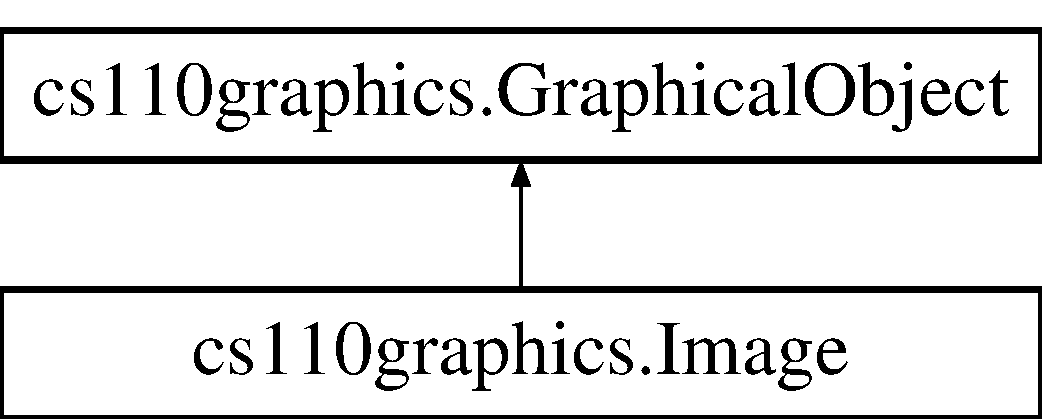
\includegraphics[height=2cm]{classcs110graphics_1_1Image}
\end{center}
\end{figure}
\subsection*{Public Member Functions}
\begin{DoxyCompactItemize}
\item 
def \hyperlink{classcs110graphics_1_1Image_a3b7c128fa18d85ff4a7586fac04a1bc2}{\_\-\_\-init\_\-\_\-}
\item 
def \hyperlink{classcs110graphics_1_1Image_a540d48247976343a91c610009a9af8cd}{move}
\begin{DoxyCompactList}\small\item\em Moves the object dx pixels horizontally and dy pixels vertically. \item\end{DoxyCompactList}\item 
def \hyperlink{classcs110graphics_1_1Image_a4b2e775fbb0cb523f6bc09028dc05c65}{move\_\-to}
\begin{DoxyCompactList}\small\item\em Moves a graphical object to a point. \item\end{DoxyCompactList}\item 
def \hyperlink{classcs110graphics_1_1Image_a0754151035bb2892f0cd3895b64488fa}{resize}
\begin{DoxyCompactList}\small\item\em Resizes the \hyperlink{classcs110graphics_1_1Image}{Image}. \item\end{DoxyCompactList}\item 
def \hyperlink{classcs110graphics_1_1Image_ac58717d68279e536cee608e2bdfc6aa8}{rotate}
\begin{DoxyCompactList}\small\item\em Rotates an object. \item\end{DoxyCompactList}\item 
def \hyperlink{classcs110graphics_1_1Image_a7a59fde33fe83916a4155fafb5cfb01e}{scale}
\begin{DoxyCompactList}\small\item\em Scales the image according to the factor. \item\end{DoxyCompactList}\item 
def \hyperlink{classcs110graphics_1_1Image_a4ff2da7a167a433f2c38f1e2e2fe7263}{size}
\begin{DoxyCompactList}\small\item\em Returns a tuple of the width and height of the image. \item\end{DoxyCompactList}\item 
def \hyperlink{classcs110graphics_1_1GraphicalObject_adb1af0d5a6baae3f9a08d21a3227c49f}{add\_\-handler}
\begin{DoxyCompactList}\small\item\em Adds a handler to the graphical object. \item\end{DoxyCompactList}\item 
def \hyperlink{classcs110graphics_1_1GraphicalObject_a062789c4cc9de38af32dcc4ff2058607}{get\_\-center}
\begin{DoxyCompactList}\small\item\em Returns the center of the object. \item\end{DoxyCompactList}\item 
def \hyperlink{classcs110graphics_1_1GraphicalObject_a6d9f5718cd0cf249e0d2842971bae17f}{get\_\-depth}
\begin{DoxyCompactList}\small\item\em Returns the depth of the object. \item\end{DoxyCompactList}\item 
def \hyperlink{classcs110graphics_1_1GraphicalObject_a20d76d4ee4419c3065d61deb6cbc6700}{set\_\-depth}
\begin{DoxyCompactList}\small\item\em Sets the depth of the \hyperlink{classcs110graphics_1_1GraphicalObject}{GraphicalObject}. \item\end{DoxyCompactList}\end{DoxyCompactItemize}


\subsection{Detailed Description}
An image, which can be added to a \hyperlink{classcs110graphics_1_1Window}{Window} object. 

\subsection{Member Function Documentation}
\hypertarget{classcs110graphics_1_1Image_a3b7c128fa18d85ff4a7586fac04a1bc2}{
\index{cs110graphics::Image@{cs110graphics::Image}!\_\-\_\-init\_\-\_\-@{\_\-\_\-init\_\-\_\-}}
\index{\_\-\_\-init\_\-\_\-@{\_\-\_\-init\_\-\_\-}!cs110graphics::Image@{cs110graphics::Image}}
\subsubsection[{\_\-\_\-init\_\-\_\-}]{\setlength{\rightskip}{0pt plus 5cm}def cs110graphics.Image.\_\-\_\-init\_\-\_\- ( {\em self}, \/   {\em window}, \/   {\em image\_\-loc}, \/   {\em width} = {\ttfamily 100}, \/   {\em height} = {\ttfamily 100}, \/   {\em center} = {\ttfamily (200,~200})}}
\label{classcs110graphics_1_1Image_a3b7c128fa18d85ff4a7586fac04a1bc2}

\begin{DoxyParams}{Parameters}
\item[{\em window}]-\/ \hyperlink{classcs110graphics_1_1Window}{Window} -\/ the window which the object will be added to \item[{\em image\_\-loc}]-\/ str-\/ The file location for an image, see below for instructions regarding file locations \item[{\em width}]-\/ int -\/ {\bfseries (default: 100)} the width of the image \item[{\em height}]-\/ int -\/ {\bfseries (default: 100)} the height of the image \item[{\em center}]-\/ tuple of (int $\ast$ int) -\/ {\bfseries (default: (200, 200))} the center location for the image\end{DoxyParams}
File locations:
\begin{DoxyItemize}
\item If a file is in the same folder/directory as the program, just use the name of the file
\item Otherwise use a file path: eg. \char`\"{}$\sim$/110/bots/images/bot.jpg\char`\"{} or \char`\"{}./images/bot.jpg\char`\"{}
\end{DoxyItemize}

Note that \char`\"{}.\char`\"{} represents the current directory and \char`\"{}..\char`\"{} represents the parent directory. \hypertarget{classcs110graphics_1_1GraphicalObject_adb1af0d5a6baae3f9a08d21a3227c49f}{
\index{cs110graphics::Image@{cs110graphics::Image}!add\_\-handler@{add\_\-handler}}
\index{add\_\-handler@{add\_\-handler}!cs110graphics::Image@{cs110graphics::Image}}
\subsubsection[{add\_\-handler}]{\setlength{\rightskip}{0pt plus 5cm}def cs110graphics.GraphicalObject.add\_\-handler ( {\em self}, \/   {\em handler\_\-object})\hspace{0.3cm}{\ttfamily  \mbox{[}inherited\mbox{]}}}}
\label{classcs110graphics_1_1GraphicalObject_adb1af0d5a6baae3f9a08d21a3227c49f}


Adds a handler to the graphical object. 
\begin{DoxyParams}{Parameters}
\item[{\em handler\_\-object}]-\/ \hyperlink{classcs110graphics_1_1EventHandler}{EventHandler} -\/ the object that handles the events for this \hyperlink{classcs110graphics_1_1GraphicalObject}{GraphicalObject} \end{DoxyParams}
\hypertarget{classcs110graphics_1_1GraphicalObject_a062789c4cc9de38af32dcc4ff2058607}{
\index{cs110graphics::Image@{cs110graphics::Image}!get\_\-center@{get\_\-center}}
\index{get\_\-center@{get\_\-center}!cs110graphics::Image@{cs110graphics::Image}}
\subsubsection[{get\_\-center}]{\setlength{\rightskip}{0pt plus 5cm}def cs110graphics.GraphicalObject.get\_\-center ( {\em self})\hspace{0.3cm}{\ttfamily  \mbox{[}inherited\mbox{]}}}}
\label{classcs110graphics_1_1GraphicalObject_a062789c4cc9de38af32dcc4ff2058607}


Returns the center of the object. \begin{DoxyReturn}{Returns}
center -\/ tuple 
\end{DoxyReturn}
\hypertarget{classcs110graphics_1_1GraphicalObject_a6d9f5718cd0cf249e0d2842971bae17f}{
\index{cs110graphics::Image@{cs110graphics::Image}!get\_\-depth@{get\_\-depth}}
\index{get\_\-depth@{get\_\-depth}!cs110graphics::Image@{cs110graphics::Image}}
\subsubsection[{get\_\-depth}]{\setlength{\rightskip}{0pt plus 5cm}def cs110graphics.GraphicalObject.get\_\-depth ( {\em self})\hspace{0.3cm}{\ttfamily  \mbox{[}inherited\mbox{]}}}}
\label{classcs110graphics_1_1GraphicalObject_a6d9f5718cd0cf249e0d2842971bae17f}


Returns the depth of the object. \begin{DoxyReturn}{Returns}
depth -\/ int 
\end{DoxyReturn}
\hypertarget{classcs110graphics_1_1Image_a540d48247976343a91c610009a9af8cd}{
\index{cs110graphics::Image@{cs110graphics::Image}!move@{move}}
\index{move@{move}!cs110graphics::Image@{cs110graphics::Image}}
\subsubsection[{move}]{\setlength{\rightskip}{0pt plus 5cm}def cs110graphics.Image.move ( {\em self}, \/   {\em dx}, \/   {\em dy})}}
\label{classcs110graphics_1_1Image_a540d48247976343a91c610009a9af8cd}


Moves the object dx pixels horizontally and dy pixels vertically. 
\begin{DoxyParams}{Parameters}
\item[{\em dx}]-\/ int \item[{\em dy}]-\/ int \end{DoxyParams}


Reimplemented from \hyperlink{classcs110graphics_1_1GraphicalObject_aa64d270fb83efa4a54e1a7953512f9cd}{cs110graphics.GraphicalObject}.\hypertarget{classcs110graphics_1_1Image_a4b2e775fbb0cb523f6bc09028dc05c65}{
\index{cs110graphics::Image@{cs110graphics::Image}!move\_\-to@{move\_\-to}}
\index{move\_\-to@{move\_\-to}!cs110graphics::Image@{cs110graphics::Image}}
\subsubsection[{move\_\-to}]{\setlength{\rightskip}{0pt plus 5cm}def cs110graphics.Image.move\_\-to ( {\em self}, \/   {\em point})}}
\label{classcs110graphics_1_1Image_a4b2e775fbb0cb523f6bc09028dc05c65}


Moves a graphical object to a point. 
\begin{DoxyParams}{Parameters}
\item[{\em point}]-\/ tuple of (int $\ast$ int) \end{DoxyParams}


Reimplemented from \hyperlink{classcs110graphics_1_1GraphicalObject_abe2d480265df7ac9447205c52c6946df}{cs110graphics.GraphicalObject}.\hypertarget{classcs110graphics_1_1Image_a0754151035bb2892f0cd3895b64488fa}{
\index{cs110graphics::Image@{cs110graphics::Image}!resize@{resize}}
\index{resize@{resize}!cs110graphics::Image@{cs110graphics::Image}}
\subsubsection[{resize}]{\setlength{\rightskip}{0pt plus 5cm}def cs110graphics.Image.resize ( {\em self}, \/   {\em width}, \/   {\em height})}}
\label{classcs110graphics_1_1Image_a0754151035bb2892f0cd3895b64488fa}


Resizes the \hyperlink{classcs110graphics_1_1Image}{Image}. 
\begin{DoxyParams}{Parameters}
\item[{\em width}]-\/ int \item[{\em height}]-\/ int \end{DoxyParams}
\hypertarget{classcs110graphics_1_1Image_ac58717d68279e536cee608e2bdfc6aa8}{
\index{cs110graphics::Image@{cs110graphics::Image}!rotate@{rotate}}
\index{rotate@{rotate}!cs110graphics::Image@{cs110graphics::Image}}
\subsubsection[{rotate}]{\setlength{\rightskip}{0pt plus 5cm}def cs110graphics.Image.rotate ( {\em self}, \/   {\em degrees})}}
\label{classcs110graphics_1_1Image_ac58717d68279e536cee608e2bdfc6aa8}


Rotates an object. 
\begin{DoxyParams}{Parameters}
\item[{\em degrees}]-\/ int \end{DoxyParams}
\hypertarget{classcs110graphics_1_1Image_a7a59fde33fe83916a4155fafb5cfb01e}{
\index{cs110graphics::Image@{cs110graphics::Image}!scale@{scale}}
\index{scale@{scale}!cs110graphics::Image@{cs110graphics::Image}}
\subsubsection[{scale}]{\setlength{\rightskip}{0pt plus 5cm}def cs110graphics.Image.scale ( {\em self}, \/   {\em factor})}}
\label{classcs110graphics_1_1Image_a7a59fde33fe83916a4155fafb5cfb01e}


Scales the image according to the factor. 
\begin{DoxyParams}{Parameters}
\item[{\em factor}]-\/ float \end{DoxyParams}
\hypertarget{classcs110graphics_1_1GraphicalObject_a20d76d4ee4419c3065d61deb6cbc6700}{
\index{cs110graphics::Image@{cs110graphics::Image}!set\_\-depth@{set\_\-depth}}
\index{set\_\-depth@{set\_\-depth}!cs110graphics::Image@{cs110graphics::Image}}
\subsubsection[{set\_\-depth}]{\setlength{\rightskip}{0pt plus 5cm}def cs110graphics.GraphicalObject.set\_\-depth ( {\em self}, \/   {\em depth})\hspace{0.3cm}{\ttfamily  \mbox{[}inherited\mbox{]}}}}
\label{classcs110graphics_1_1GraphicalObject_a20d76d4ee4419c3065d61deb6cbc6700}


Sets the depth of the \hyperlink{classcs110graphics_1_1GraphicalObject}{GraphicalObject}. 
\begin{DoxyParams}{Parameters}
\item[{\em depth}]-\/ int \end{DoxyParams}
\hypertarget{classcs110graphics_1_1Image_a4ff2da7a167a433f2c38f1e2e2fe7263}{
\index{cs110graphics::Image@{cs110graphics::Image}!size@{size}}
\index{size@{size}!cs110graphics::Image@{cs110graphics::Image}}
\subsubsection[{size}]{\setlength{\rightskip}{0pt plus 5cm}def cs110graphics.Image.size ( {\em self})}}
\label{classcs110graphics_1_1Image_a4ff2da7a167a433f2c38f1e2e2fe7263}


Returns a tuple of the width and height of the image. \begin{DoxyReturn}{Returns}
size -\/ tuple of (int $\ast$ int) 
\end{DoxyReturn}


The documentation for this class was generated from the following file:\begin{DoxyCompactItemize}
\item 
\hyperlink{cs110graphics_8py}{cs110graphics.py}\end{DoxyCompactItemize}

\hypertarget{classcs110graphics_1_1Oval}{
\section{cs110graphics.Oval Class Reference}
\label{classcs110graphics_1_1Oval}\index{cs110graphics::Oval@{cs110graphics::Oval}}
}


An oval, which can be added to a \hyperlink{classcs110graphics_1_1Window}{Window} object.  
Inheritance diagram for cs110graphics.Oval::\begin{figure}[H]
\begin{center}
\leavevmode
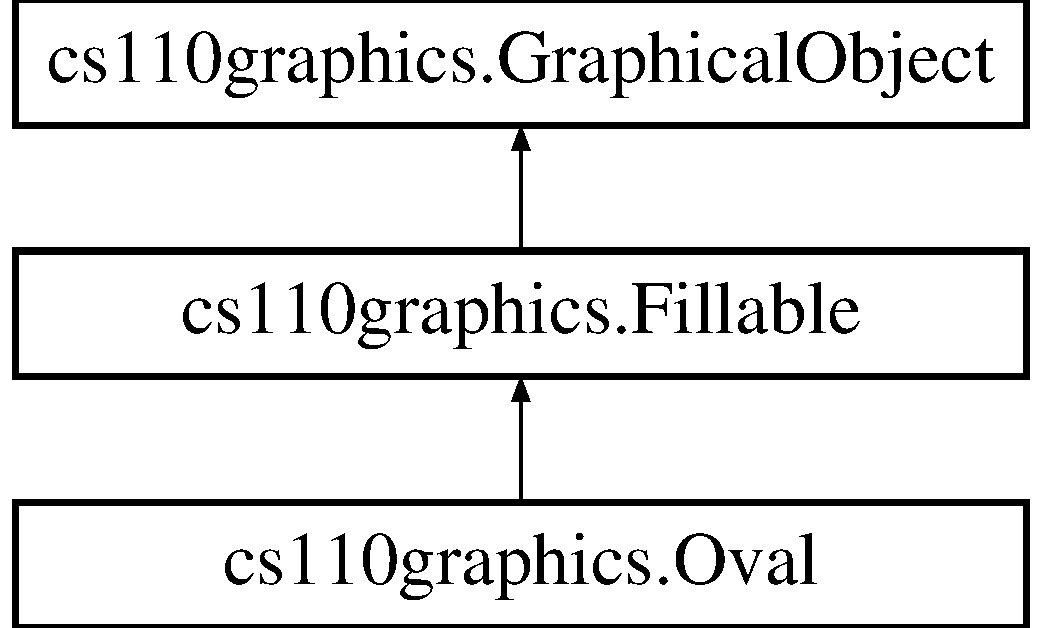
\includegraphics[height=3cm]{classcs110graphics_1_1Oval}
\end{center}
\end{figure}
\subsection*{Public Member Functions}
\begin{DoxyCompactItemize}
\item 
def \hyperlink{classcs110graphics_1_1Oval_a7f71ea6ad224b510456c9de76e72ff11}{\_\-\_\-init\_\-\_\-}
\item 
def \hyperlink{classcs110graphics_1_1Oval_a5d699cffc26c514e0eb9bdfde9a2951b}{set\_\-radii}
\begin{DoxyCompactList}\small\item\em Sets the horizontal and vertical radii of the oval. \item\end{DoxyCompactList}\item 
def \hyperlink{classcs110graphics_1_1Fillable_a6772d56158c9fe98a33f01d47cb8aa41}{get\_\-border\_\-color}
\begin{DoxyCompactList}\small\item\em Returns the border color. \item\end{DoxyCompactList}\item 
def \hyperlink{classcs110graphics_1_1Fillable_a6ed7a4288e84a090ec185c8bdff21d0f}{get\_\-border\_\-width}
\begin{DoxyCompactList}\small\item\em Returns the border width. \item\end{DoxyCompactList}\item 
def \hyperlink{classcs110graphics_1_1Fillable_a16c045bc9b63961b696914ee1a1d14d9}{get\_\-fill\_\-color}
\begin{DoxyCompactList}\small\item\em Returns fill color. \item\end{DoxyCompactList}\item 
def \hyperlink{classcs110graphics_1_1Fillable_a514fa0d21297c1372681afae9219fd58}{get\_\-pivot}
\begin{DoxyCompactList}\small\item\em Returns the pivot point. \item\end{DoxyCompactList}\item 
def \hyperlink{classcs110graphics_1_1Fillable_afa6710f6c314de39d19f06d9dd306d7d}{rotate}
\begin{DoxyCompactList}\small\item\em Rotates the object. \item\end{DoxyCompactList}\item 
def \hyperlink{classcs110graphics_1_1Fillable_a80d5b6b6d2ebae867dccecb803075749}{scale}
\begin{DoxyCompactList}\small\item\em Scales the object up or down depending on the factor. \item\end{DoxyCompactList}\item 
def \hyperlink{classcs110graphics_1_1Fillable_ae8f6c476e29c0810453dc16948e1730c}{move}
\begin{DoxyCompactList}\small\item\em Moves the object dx pixels horizontally and dy pixels vertically. \item\end{DoxyCompactList}\item 
def \hyperlink{classcs110graphics_1_1Fillable_adcabc14e76d1160ff591b9ef7f3d6a97}{move\_\-to}
\begin{DoxyCompactList}\small\item\em Moves a graphical object to a point. \item\end{DoxyCompactList}\item 
def \hyperlink{classcs110graphics_1_1Fillable_a2f830be5d970faac97759910d20d68a4}{set\_\-border\_\-color}
\begin{DoxyCompactList}\small\item\em Sets the border color. \item\end{DoxyCompactList}\item 
def \hyperlink{classcs110graphics_1_1Fillable_a09f05462cb2ed38fdccb244340f05b2b}{set\_\-border\_\-width}
\begin{DoxyCompactList}\small\item\em Sets the border width. \item\end{DoxyCompactList}\item 
def \hyperlink{classcs110graphics_1_1Fillable_a4f24c7186c8d057e42a0209eb1d56be7}{set\_\-fill\_\-color}
\begin{DoxyCompactList}\small\item\em Sets the fill color. \item\end{DoxyCompactList}\item 
def \hyperlink{classcs110graphics_1_1Fillable_a2a6066d1a11c0854ff5ee85e7d9ceb54}{set\_\-pivot}
\begin{DoxyCompactList}\small\item\em Sets the pivot point. \item\end{DoxyCompactList}\item 
def \hyperlink{classcs110graphics_1_1GraphicalObject_adb1af0d5a6baae3f9a08d21a3227c49f}{add\_\-handler}
\begin{DoxyCompactList}\small\item\em Adds a handler to the graphical object. \item\end{DoxyCompactList}\item 
def \hyperlink{classcs110graphics_1_1GraphicalObject_a062789c4cc9de38af32dcc4ff2058607}{get\_\-center}
\begin{DoxyCompactList}\small\item\em Returns the center of the object. \item\end{DoxyCompactList}\item 
def \hyperlink{classcs110graphics_1_1GraphicalObject_a6d9f5718cd0cf249e0d2842971bae17f}{get\_\-depth}
\begin{DoxyCompactList}\small\item\em Returns the depth of the object. \item\end{DoxyCompactList}\item 
def \hyperlink{classcs110graphics_1_1GraphicalObject_a20d76d4ee4419c3065d61deb6cbc6700}{set\_\-depth}
\begin{DoxyCompactList}\small\item\em Sets the depth of the \hyperlink{classcs110graphics_1_1GraphicalObject}{GraphicalObject}. \item\end{DoxyCompactList}\end{DoxyCompactItemize}


\subsection{Detailed Description}
An oval, which can be added to a \hyperlink{classcs110graphics_1_1Window}{Window} object. 

\subsection{Member Function Documentation}
\hypertarget{classcs110graphics_1_1Oval_a7f71ea6ad224b510456c9de76e72ff11}{
\index{cs110graphics::Oval@{cs110graphics::Oval}!\_\-\_\-init\_\-\_\-@{\_\-\_\-init\_\-\_\-}}
\index{\_\-\_\-init\_\-\_\-@{\_\-\_\-init\_\-\_\-}!cs110graphics::Oval@{cs110graphics::Oval}}
\subsubsection[{\_\-\_\-init\_\-\_\-}]{\setlength{\rightskip}{0pt plus 5cm}def cs110graphics.Oval.\_\-\_\-init\_\-\_\- ( {\em self}, \/   {\em window}, \/   {\em radiusX} = {\ttfamily 40}, \/   {\em radiusY} = {\ttfamily 60}, \/   {\em center} = {\ttfamily (200,~200})}}
\label{classcs110graphics_1_1Oval_a7f71ea6ad224b510456c9de76e72ff11}

\begin{DoxyParams}{Parameters}
\item[{\em window}]-\/ \hyperlink{classcs110graphics_1_1Window}{Window} -\/ the window which the object will be added to \item[{\em radiusX}]-\/ int -\/ {\bfseries (default: 40)} the radius in the x-\/direction \item[{\em radiusY}]-\/ int -\/ {\bfseries (default: 60)} the radius in the y-\/direction \item[{\em center}]-\/ tuple of (int $\ast$ int) -\/ {\bfseries (default: (200, 200))} the center of the oval \end{DoxyParams}
\hypertarget{classcs110graphics_1_1GraphicalObject_adb1af0d5a6baae3f9a08d21a3227c49f}{
\index{cs110graphics::Oval@{cs110graphics::Oval}!add\_\-handler@{add\_\-handler}}
\index{add\_\-handler@{add\_\-handler}!cs110graphics::Oval@{cs110graphics::Oval}}
\subsubsection[{add\_\-handler}]{\setlength{\rightskip}{0pt plus 5cm}def cs110graphics.GraphicalObject.add\_\-handler ( {\em self}, \/   {\em handler\_\-object})\hspace{0.3cm}{\ttfamily  \mbox{[}inherited\mbox{]}}}}
\label{classcs110graphics_1_1GraphicalObject_adb1af0d5a6baae3f9a08d21a3227c49f}


Adds a handler to the graphical object. 
\begin{DoxyParams}{Parameters}
\item[{\em handler\_\-object}]-\/ \hyperlink{classcs110graphics_1_1EventHandler}{EventHandler} -\/ the object that handles the events for this \hyperlink{classcs110graphics_1_1GraphicalObject}{GraphicalObject} \end{DoxyParams}
\hypertarget{classcs110graphics_1_1Fillable_a6772d56158c9fe98a33f01d47cb8aa41}{
\index{cs110graphics::Oval@{cs110graphics::Oval}!get\_\-border\_\-color@{get\_\-border\_\-color}}
\index{get\_\-border\_\-color@{get\_\-border\_\-color}!cs110graphics::Oval@{cs110graphics::Oval}}
\subsubsection[{get\_\-border\_\-color}]{\setlength{\rightskip}{0pt plus 5cm}def cs110graphics.Fillable.get\_\-border\_\-color ( {\em self})\hspace{0.3cm}{\ttfamily  \mbox{[}inherited\mbox{]}}}}
\label{classcs110graphics_1_1Fillable_a6772d56158c9fe98a33f01d47cb8aa41}


Returns the border color. \begin{DoxyReturn}{Returns}
border\_\-color -\/ str -\/ Can be either the name of a color (\char`\"{}yellow\char`\"{}), or a hex code (\char`\"{}\#FFFF00\char`\"{}) 
\end{DoxyReturn}
\hypertarget{classcs110graphics_1_1Fillable_a6ed7a4288e84a090ec185c8bdff21d0f}{
\index{cs110graphics::Oval@{cs110graphics::Oval}!get\_\-border\_\-width@{get\_\-border\_\-width}}
\index{get\_\-border\_\-width@{get\_\-border\_\-width}!cs110graphics::Oval@{cs110graphics::Oval}}
\subsubsection[{get\_\-border\_\-width}]{\setlength{\rightskip}{0pt plus 5cm}def cs110graphics.Fillable.get\_\-border\_\-width ( {\em self})\hspace{0.3cm}{\ttfamily  \mbox{[}inherited\mbox{]}}}}
\label{classcs110graphics_1_1Fillable_a6ed7a4288e84a090ec185c8bdff21d0f}


Returns the border width. \begin{DoxyReturn}{Returns}
border\_\-width -\/ int 
\end{DoxyReturn}
\hypertarget{classcs110graphics_1_1GraphicalObject_a062789c4cc9de38af32dcc4ff2058607}{
\index{cs110graphics::Oval@{cs110graphics::Oval}!get\_\-center@{get\_\-center}}
\index{get\_\-center@{get\_\-center}!cs110graphics::Oval@{cs110graphics::Oval}}
\subsubsection[{get\_\-center}]{\setlength{\rightskip}{0pt plus 5cm}def cs110graphics.GraphicalObject.get\_\-center ( {\em self})\hspace{0.3cm}{\ttfamily  \mbox{[}inherited\mbox{]}}}}
\label{classcs110graphics_1_1GraphicalObject_a062789c4cc9de38af32dcc4ff2058607}


Returns the center of the object. \begin{DoxyReturn}{Returns}
center -\/ tuple 
\end{DoxyReturn}
\hypertarget{classcs110graphics_1_1GraphicalObject_a6d9f5718cd0cf249e0d2842971bae17f}{
\index{cs110graphics::Oval@{cs110graphics::Oval}!get\_\-depth@{get\_\-depth}}
\index{get\_\-depth@{get\_\-depth}!cs110graphics::Oval@{cs110graphics::Oval}}
\subsubsection[{get\_\-depth}]{\setlength{\rightskip}{0pt plus 5cm}def cs110graphics.GraphicalObject.get\_\-depth ( {\em self})\hspace{0.3cm}{\ttfamily  \mbox{[}inherited\mbox{]}}}}
\label{classcs110graphics_1_1GraphicalObject_a6d9f5718cd0cf249e0d2842971bae17f}


Returns the depth of the object. \begin{DoxyReturn}{Returns}
depth -\/ int 
\end{DoxyReturn}
\hypertarget{classcs110graphics_1_1Fillable_a16c045bc9b63961b696914ee1a1d14d9}{
\index{cs110graphics::Oval@{cs110graphics::Oval}!get\_\-fill\_\-color@{get\_\-fill\_\-color}}
\index{get\_\-fill\_\-color@{get\_\-fill\_\-color}!cs110graphics::Oval@{cs110graphics::Oval}}
\subsubsection[{get\_\-fill\_\-color}]{\setlength{\rightskip}{0pt plus 5cm}def cs110graphics.Fillable.get\_\-fill\_\-color ( {\em self})\hspace{0.3cm}{\ttfamily  \mbox{[}inherited\mbox{]}}}}
\label{classcs110graphics_1_1Fillable_a16c045bc9b63961b696914ee1a1d14d9}


Returns fill color. \begin{DoxyReturn}{Returns}
color -\/ int -\/ Can be either the name of a color (\char`\"{}yellow\char`\"{}), or a hex code (\char`\"{}\#FFFF00\char`\"{}) 
\end{DoxyReturn}
\hypertarget{classcs110graphics_1_1Fillable_a514fa0d21297c1372681afae9219fd58}{
\index{cs110graphics::Oval@{cs110graphics::Oval}!get\_\-pivot@{get\_\-pivot}}
\index{get\_\-pivot@{get\_\-pivot}!cs110graphics::Oval@{cs110graphics::Oval}}
\subsubsection[{get\_\-pivot}]{\setlength{\rightskip}{0pt plus 5cm}def cs110graphics.Fillable.get\_\-pivot ( {\em self})\hspace{0.3cm}{\ttfamily  \mbox{[}inherited\mbox{]}}}}
\label{classcs110graphics_1_1Fillable_a514fa0d21297c1372681afae9219fd58}


Returns the pivot point. \begin{DoxyReturn}{Returns}
pivot -\/ tuple (int $\ast$ int) 
\end{DoxyReturn}
\hypertarget{classcs110graphics_1_1Fillable_ae8f6c476e29c0810453dc16948e1730c}{
\index{cs110graphics::Oval@{cs110graphics::Oval}!move@{move}}
\index{move@{move}!cs110graphics::Oval@{cs110graphics::Oval}}
\subsubsection[{move}]{\setlength{\rightskip}{0pt plus 5cm}def cs110graphics.Fillable.move ( {\em self}, \/   {\em dx}, \/   {\em dy})\hspace{0.3cm}{\ttfamily  \mbox{[}inherited\mbox{]}}}}
\label{classcs110graphics_1_1Fillable_ae8f6c476e29c0810453dc16948e1730c}


Moves the object dx pixels horizontally and dy pixels vertically. 
\begin{DoxyParams}{Parameters}
\item[{\em dx}]-\/ int \item[{\em dy}]-\/ int \end{DoxyParams}


Reimplemented from \hyperlink{classcs110graphics_1_1GraphicalObject_aa64d270fb83efa4a54e1a7953512f9cd}{cs110graphics.GraphicalObject}.\hypertarget{classcs110graphics_1_1Fillable_adcabc14e76d1160ff591b9ef7f3d6a97}{
\index{cs110graphics::Oval@{cs110graphics::Oval}!move\_\-to@{move\_\-to}}
\index{move\_\-to@{move\_\-to}!cs110graphics::Oval@{cs110graphics::Oval}}
\subsubsection[{move\_\-to}]{\setlength{\rightskip}{0pt plus 5cm}def cs110graphics.Fillable.move\_\-to ( {\em self}, \/   {\em point})\hspace{0.3cm}{\ttfamily  \mbox{[}inherited\mbox{]}}}}
\label{classcs110graphics_1_1Fillable_adcabc14e76d1160ff591b9ef7f3d6a97}


Moves a graphical object to a point. 
\begin{DoxyParams}{Parameters}
\item[{\em point}]-\/ tuple of (int $\ast$ int) \end{DoxyParams}


Reimplemented from \hyperlink{classcs110graphics_1_1GraphicalObject_abe2d480265df7ac9447205c52c6946df}{cs110graphics.GraphicalObject}.\hypertarget{classcs110graphics_1_1Fillable_afa6710f6c314de39d19f06d9dd306d7d}{
\index{cs110graphics::Oval@{cs110graphics::Oval}!rotate@{rotate}}
\index{rotate@{rotate}!cs110graphics::Oval@{cs110graphics::Oval}}
\subsubsection[{rotate}]{\setlength{\rightskip}{0pt plus 5cm}def cs110graphics.Fillable.rotate ( {\em self}, \/   {\em degrees})\hspace{0.3cm}{\ttfamily  \mbox{[}inherited\mbox{]}}}}
\label{classcs110graphics_1_1Fillable_afa6710f6c314de39d19f06d9dd306d7d}


Rotates the object. 
\begin{DoxyParams}{Parameters}
\item[{\em degrees}]-\/ int \end{DoxyParams}
\hypertarget{classcs110graphics_1_1Fillable_a80d5b6b6d2ebae867dccecb803075749}{
\index{cs110graphics::Oval@{cs110graphics::Oval}!scale@{scale}}
\index{scale@{scale}!cs110graphics::Oval@{cs110graphics::Oval}}
\subsubsection[{scale}]{\setlength{\rightskip}{0pt plus 5cm}def cs110graphics.Fillable.scale ( {\em self}, \/   {\em factor})\hspace{0.3cm}{\ttfamily  \mbox{[}inherited\mbox{]}}}}
\label{classcs110graphics_1_1Fillable_a80d5b6b6d2ebae867dccecb803075749}


Scales the object up or down depending on the factor. 
\begin{DoxyParams}{Parameters}
\item[{\em factor}]-\/ float \end{DoxyParams}
\hypertarget{classcs110graphics_1_1Fillable_a2f830be5d970faac97759910d20d68a4}{
\index{cs110graphics::Oval@{cs110graphics::Oval}!set\_\-border\_\-color@{set\_\-border\_\-color}}
\index{set\_\-border\_\-color@{set\_\-border\_\-color}!cs110graphics::Oval@{cs110graphics::Oval}}
\subsubsection[{set\_\-border\_\-color}]{\setlength{\rightskip}{0pt plus 5cm}def cs110graphics.Fillable.set\_\-border\_\-color ( {\em self}, \/   {\em color})\hspace{0.3cm}{\ttfamily  \mbox{[}inherited\mbox{]}}}}
\label{classcs110graphics_1_1Fillable_a2f830be5d970faac97759910d20d68a4}


Sets the border color. 
\begin{DoxyParams}{Parameters}
\item[{\em color}]-\/ string -\/ Can be either the name of a color (\char`\"{}yellow\char`\"{}), or a hex code (\char`\"{}\#FFFF00\char`\"{}) \end{DoxyParams}
\hypertarget{classcs110graphics_1_1Fillable_a09f05462cb2ed38fdccb244340f05b2b}{
\index{cs110graphics::Oval@{cs110graphics::Oval}!set\_\-border\_\-width@{set\_\-border\_\-width}}
\index{set\_\-border\_\-width@{set\_\-border\_\-width}!cs110graphics::Oval@{cs110graphics::Oval}}
\subsubsection[{set\_\-border\_\-width}]{\setlength{\rightskip}{0pt plus 5cm}def cs110graphics.Fillable.set\_\-border\_\-width ( {\em self}, \/   {\em width})\hspace{0.3cm}{\ttfamily  \mbox{[}inherited\mbox{]}}}}
\label{classcs110graphics_1_1Fillable_a09f05462cb2ed38fdccb244340f05b2b}


Sets the border width. 
\begin{DoxyParams}{Parameters}
\item[{\em width}]-\/ int \end{DoxyParams}
\hypertarget{classcs110graphics_1_1GraphicalObject_a20d76d4ee4419c3065d61deb6cbc6700}{
\index{cs110graphics::Oval@{cs110graphics::Oval}!set\_\-depth@{set\_\-depth}}
\index{set\_\-depth@{set\_\-depth}!cs110graphics::Oval@{cs110graphics::Oval}}
\subsubsection[{set\_\-depth}]{\setlength{\rightskip}{0pt plus 5cm}def cs110graphics.GraphicalObject.set\_\-depth ( {\em self}, \/   {\em depth})\hspace{0.3cm}{\ttfamily  \mbox{[}inherited\mbox{]}}}}
\label{classcs110graphics_1_1GraphicalObject_a20d76d4ee4419c3065d61deb6cbc6700}


Sets the depth of the \hyperlink{classcs110graphics_1_1GraphicalObject}{GraphicalObject}. 
\begin{DoxyParams}{Parameters}
\item[{\em depth}]-\/ int \end{DoxyParams}
\hypertarget{classcs110graphics_1_1Fillable_a4f24c7186c8d057e42a0209eb1d56be7}{
\index{cs110graphics::Oval@{cs110graphics::Oval}!set\_\-fill\_\-color@{set\_\-fill\_\-color}}
\index{set\_\-fill\_\-color@{set\_\-fill\_\-color}!cs110graphics::Oval@{cs110graphics::Oval}}
\subsubsection[{set\_\-fill\_\-color}]{\setlength{\rightskip}{0pt plus 5cm}def cs110graphics.Fillable.set\_\-fill\_\-color ( {\em self}, \/   {\em color})\hspace{0.3cm}{\ttfamily  \mbox{[}inherited\mbox{]}}}}
\label{classcs110graphics_1_1Fillable_a4f24c7186c8d057e42a0209eb1d56be7}


Sets the fill color. 
\begin{DoxyParams}{Parameters}
\item[{\em color}]-\/ string -\/ Can be either the name of a color (\char`\"{}yellow\char`\"{}), or a hex code (\char`\"{}\#FFFF00\char`\"{}) \end{DoxyParams}
\hypertarget{classcs110graphics_1_1Fillable_a2a6066d1a11c0854ff5ee85e7d9ceb54}{
\index{cs110graphics::Oval@{cs110graphics::Oval}!set\_\-pivot@{set\_\-pivot}}
\index{set\_\-pivot@{set\_\-pivot}!cs110graphics::Oval@{cs110graphics::Oval}}
\subsubsection[{set\_\-pivot}]{\setlength{\rightskip}{0pt plus 5cm}def cs110graphics.Fillable.set\_\-pivot ( {\em self}, \/   {\em pivot})\hspace{0.3cm}{\ttfamily  \mbox{[}inherited\mbox{]}}}}
\label{classcs110graphics_1_1Fillable_a2a6066d1a11c0854ff5ee85e7d9ceb54}


Sets the pivot point. 
\begin{DoxyParams}{Parameters}
\item[{\em pivot}]-\/ tuple of (int $\ast$ int) \end{DoxyParams}
\hypertarget{classcs110graphics_1_1Oval_a5d699cffc26c514e0eb9bdfde9a2951b}{
\index{cs110graphics::Oval@{cs110graphics::Oval}!set\_\-radii@{set\_\-radii}}
\index{set\_\-radii@{set\_\-radii}!cs110graphics::Oval@{cs110graphics::Oval}}
\subsubsection[{set\_\-radii}]{\setlength{\rightskip}{0pt plus 5cm}def cs110graphics.Oval.set\_\-radii ( {\em self}, \/   {\em radiusX}, \/   {\em radiusY})}}
\label{classcs110graphics_1_1Oval_a5d699cffc26c514e0eb9bdfde9a2951b}


Sets the horizontal and vertical radii of the oval. 
\begin{DoxyParams}{Parameters}
\item[{\em radiusX}]-\/ int \item[{\em radiusY}]-\/ int \end{DoxyParams}


The documentation for this class was generated from the following file:\begin{DoxyCompactItemize}
\item 
\hyperlink{cs110graphics_8py}{cs110graphics.py}\end{DoxyCompactItemize}

\hypertarget{classcs110graphics_1_1Polygon}{
\section{cs110graphics.Polygon Class Reference}
\label{classcs110graphics_1_1Polygon}\index{cs110graphics::Polygon@{cs110graphics::Polygon}}
}


A \hyperlink{classcs110graphics_1_1Polygon}{Polygon}, which can be added to a \hyperlink{classcs110graphics_1_1Window}{Window} object.  
Inheritance diagram for cs110graphics.Polygon::\begin{figure}[H]
\begin{center}
\leavevmode
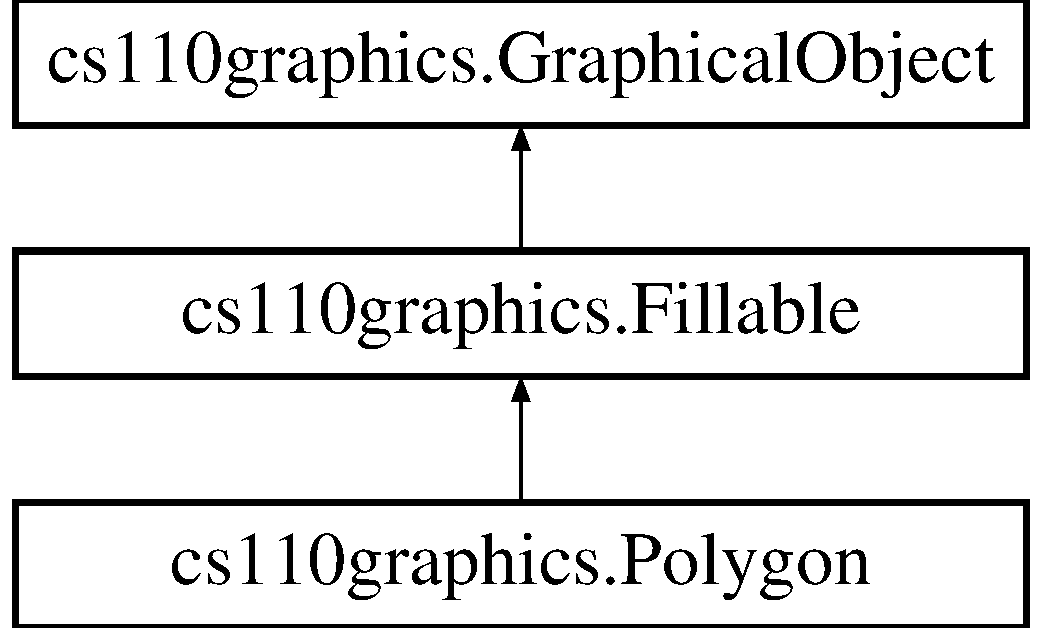
\includegraphics[height=3cm]{classcs110graphics_1_1Polygon}
\end{center}
\end{figure}
\subsection*{Public Member Functions}
\begin{DoxyCompactItemize}
\item 
def \hyperlink{classcs110graphics_1_1Polygon_ab471e73072b87896eec42f385102c800}{\_\-\_\-init\_\-\_\-}
\item 
def \hyperlink{classcs110graphics_1_1Fillable_a6772d56158c9fe98a33f01d47cb8aa41}{get\_\-border\_\-color}
\begin{DoxyCompactList}\small\item\em Returns the border color. \item\end{DoxyCompactList}\item 
def \hyperlink{classcs110graphics_1_1Fillable_a6ed7a4288e84a090ec185c8bdff21d0f}{get\_\-border\_\-width}
\begin{DoxyCompactList}\small\item\em Returns the border width. \item\end{DoxyCompactList}\item 
def \hyperlink{classcs110graphics_1_1Fillable_a16c045bc9b63961b696914ee1a1d14d9}{get\_\-fill\_\-color}
\begin{DoxyCompactList}\small\item\em Returns fill color. \item\end{DoxyCompactList}\item 
def \hyperlink{classcs110graphics_1_1Fillable_a514fa0d21297c1372681afae9219fd58}{get\_\-pivot}
\begin{DoxyCompactList}\small\item\em Returns the pivot point. \item\end{DoxyCompactList}\item 
def \hyperlink{classcs110graphics_1_1Fillable_afa6710f6c314de39d19f06d9dd306d7d}{rotate}
\begin{DoxyCompactList}\small\item\em Rotates the object. \item\end{DoxyCompactList}\item 
def \hyperlink{classcs110graphics_1_1Fillable_a80d5b6b6d2ebae867dccecb803075749}{scale}
\begin{DoxyCompactList}\small\item\em Scales the object up or down depending on the factor. \item\end{DoxyCompactList}\item 
def \hyperlink{classcs110graphics_1_1Fillable_a2f830be5d970faac97759910d20d68a4}{set\_\-border\_\-color}
\begin{DoxyCompactList}\small\item\em Sets the border color. \item\end{DoxyCompactList}\item 
def \hyperlink{classcs110graphics_1_1Fillable_a09f05462cb2ed38fdccb244340f05b2b}{set\_\-border\_\-width}
\begin{DoxyCompactList}\small\item\em Sets the border width. \item\end{DoxyCompactList}\item 
def \hyperlink{classcs110graphics_1_1Fillable_a4f24c7186c8d057e42a0209eb1d56be7}{set\_\-fill\_\-color}
\begin{DoxyCompactList}\small\item\em Sets the fill color. \item\end{DoxyCompactList}\item 
def \hyperlink{classcs110graphics_1_1Fillable_a2a6066d1a11c0854ff5ee85e7d9ceb54}{set\_\-pivot}
\begin{DoxyCompactList}\small\item\em Sets the pivot point. \item\end{DoxyCompactList}\item 
def \hyperlink{classcs110graphics_1_1GraphicalObject_adb1af0d5a6baae3f9a08d21a3227c49f}{add\_\-handler}
\begin{DoxyCompactList}\small\item\em Adds a handler to the graphical object. \item\end{DoxyCompactList}\item 
def \hyperlink{classcs110graphics_1_1GraphicalObject_a062789c4cc9de38af32dcc4ff2058607}{get\_\-center}
\begin{DoxyCompactList}\small\item\em Returns the center of the object. \item\end{DoxyCompactList}\item 
def \hyperlink{classcs110graphics_1_1GraphicalObject_a6d9f5718cd0cf249e0d2842971bae17f}{get\_\-depth}
\begin{DoxyCompactList}\small\item\em Returns the depth of the object. \item\end{DoxyCompactList}\item 
def \hyperlink{classcs110graphics_1_1GraphicalObject_aa64d270fb83efa4a54e1a7953512f9cd}{move}
\begin{DoxyCompactList}\small\item\em Moves the object dx pixels horizontally and dy pixels vertically. \item\end{DoxyCompactList}\item 
def \hyperlink{classcs110graphics_1_1GraphicalObject_abe2d480265df7ac9447205c52c6946df}{move\_\-to}
\begin{DoxyCompactList}\small\item\em Moves a graphical object to a point. \item\end{DoxyCompactList}\item 
def \hyperlink{classcs110graphics_1_1GraphicalObject_a20d76d4ee4419c3065d61deb6cbc6700}{set\_\-depth}
\begin{DoxyCompactList}\small\item\em Sets the depth of the \hyperlink{classcs110graphics_1_1GraphicalObject}{GraphicalObject}. \item\end{DoxyCompactList}\end{DoxyCompactItemize}


\subsection{Detailed Description}
A \hyperlink{classcs110graphics_1_1Polygon}{Polygon}, which can be added to a \hyperlink{classcs110graphics_1_1Window}{Window} object. 

\subsection{Member Function Documentation}
\hypertarget{classcs110graphics_1_1Polygon_ab471e73072b87896eec42f385102c800}{
\index{cs110graphics::Polygon@{cs110graphics::Polygon}!\_\-\_\-init\_\-\_\-@{\_\-\_\-init\_\-\_\-}}
\index{\_\-\_\-init\_\-\_\-@{\_\-\_\-init\_\-\_\-}!cs110graphics::Polygon@{cs110graphics::Polygon}}
\subsubsection[{\_\-\_\-init\_\-\_\-}]{\setlength{\rightskip}{0pt plus 5cm}def cs110graphics.Polygon.\_\-\_\-init\_\-\_\- ( {\em self}, \/   {\em window}, \/   {\em points})}}
\label{classcs110graphics_1_1Polygon_ab471e73072b87896eec42f385102c800}

\begin{DoxyParams}{Parameters}
\item[{\em window}]-\/ \hyperlink{classcs110graphics_1_1Window}{Window} -\/ the window which the object will be added to \item[{\em points}]-\/ list of tuples of (int $\ast$ int) -\/ each tuple corresponds to an x-\/y point \end{DoxyParams}
\hypertarget{classcs110graphics_1_1GraphicalObject_adb1af0d5a6baae3f9a08d21a3227c49f}{
\index{cs110graphics::Polygon@{cs110graphics::Polygon}!add\_\-handler@{add\_\-handler}}
\index{add\_\-handler@{add\_\-handler}!cs110graphics::Polygon@{cs110graphics::Polygon}}
\subsubsection[{add\_\-handler}]{\setlength{\rightskip}{0pt plus 5cm}def cs110graphics.GraphicalObject.add\_\-handler ( {\em self}, \/   {\em handler\_\-object})\hspace{0.3cm}{\ttfamily  \mbox{[}inherited\mbox{]}}}}
\label{classcs110graphics_1_1GraphicalObject_adb1af0d5a6baae3f9a08d21a3227c49f}


Adds a handler to the graphical object. 
\begin{DoxyParams}{Parameters}
\item[{\em handler\_\-object}]-\/ \hyperlink{classcs110graphics_1_1EventHandler}{EventHandler} -\/ the object that handles the events for this \hyperlink{classcs110graphics_1_1GraphicalObject}{GraphicalObject} \end{DoxyParams}
\hypertarget{classcs110graphics_1_1Fillable_a6772d56158c9fe98a33f01d47cb8aa41}{
\index{cs110graphics::Polygon@{cs110graphics::Polygon}!get\_\-border\_\-color@{get\_\-border\_\-color}}
\index{get\_\-border\_\-color@{get\_\-border\_\-color}!cs110graphics::Polygon@{cs110graphics::Polygon}}
\subsubsection[{get\_\-border\_\-color}]{\setlength{\rightskip}{0pt plus 5cm}def cs110graphics.Fillable.get\_\-border\_\-color ( {\em self})\hspace{0.3cm}{\ttfamily  \mbox{[}inherited\mbox{]}}}}
\label{classcs110graphics_1_1Fillable_a6772d56158c9fe98a33f01d47cb8aa41}


Returns the border color. \begin{DoxyReturn}{Returns}
border\_\-color -\/ str -\/ Can be either the name of a color (\char`\"{}yellow\char`\"{}), or a hex code (\char`\"{}\#FFFF00\char`\"{}) 
\end{DoxyReturn}
\hypertarget{classcs110graphics_1_1Fillable_a6ed7a4288e84a090ec185c8bdff21d0f}{
\index{cs110graphics::Polygon@{cs110graphics::Polygon}!get\_\-border\_\-width@{get\_\-border\_\-width}}
\index{get\_\-border\_\-width@{get\_\-border\_\-width}!cs110graphics::Polygon@{cs110graphics::Polygon}}
\subsubsection[{get\_\-border\_\-width}]{\setlength{\rightskip}{0pt plus 5cm}def cs110graphics.Fillable.get\_\-border\_\-width ( {\em self})\hspace{0.3cm}{\ttfamily  \mbox{[}inherited\mbox{]}}}}
\label{classcs110graphics_1_1Fillable_a6ed7a4288e84a090ec185c8bdff21d0f}


Returns the border width. \begin{DoxyReturn}{Returns}
border\_\-width -\/ int 
\end{DoxyReturn}
\hypertarget{classcs110graphics_1_1GraphicalObject_a062789c4cc9de38af32dcc4ff2058607}{
\index{cs110graphics::Polygon@{cs110graphics::Polygon}!get\_\-center@{get\_\-center}}
\index{get\_\-center@{get\_\-center}!cs110graphics::Polygon@{cs110graphics::Polygon}}
\subsubsection[{get\_\-center}]{\setlength{\rightskip}{0pt plus 5cm}def cs110graphics.GraphicalObject.get\_\-center ( {\em self})\hspace{0.3cm}{\ttfamily  \mbox{[}inherited\mbox{]}}}}
\label{classcs110graphics_1_1GraphicalObject_a062789c4cc9de38af32dcc4ff2058607}


Returns the center of the object. \begin{DoxyReturn}{Returns}
center -\/ tuple 
\end{DoxyReturn}
\hypertarget{classcs110graphics_1_1GraphicalObject_a6d9f5718cd0cf249e0d2842971bae17f}{
\index{cs110graphics::Polygon@{cs110graphics::Polygon}!get\_\-depth@{get\_\-depth}}
\index{get\_\-depth@{get\_\-depth}!cs110graphics::Polygon@{cs110graphics::Polygon}}
\subsubsection[{get\_\-depth}]{\setlength{\rightskip}{0pt plus 5cm}def cs110graphics.GraphicalObject.get\_\-depth ( {\em self})\hspace{0.3cm}{\ttfamily  \mbox{[}inherited\mbox{]}}}}
\label{classcs110graphics_1_1GraphicalObject_a6d9f5718cd0cf249e0d2842971bae17f}


Returns the depth of the object. \begin{DoxyReturn}{Returns}
depth -\/ int 
\end{DoxyReturn}
\hypertarget{classcs110graphics_1_1Fillable_a16c045bc9b63961b696914ee1a1d14d9}{
\index{cs110graphics::Polygon@{cs110graphics::Polygon}!get\_\-fill\_\-color@{get\_\-fill\_\-color}}
\index{get\_\-fill\_\-color@{get\_\-fill\_\-color}!cs110graphics::Polygon@{cs110graphics::Polygon}}
\subsubsection[{get\_\-fill\_\-color}]{\setlength{\rightskip}{0pt plus 5cm}def cs110graphics.Fillable.get\_\-fill\_\-color ( {\em self})\hspace{0.3cm}{\ttfamily  \mbox{[}inherited\mbox{]}}}}
\label{classcs110graphics_1_1Fillable_a16c045bc9b63961b696914ee1a1d14d9}


Returns fill color. \begin{DoxyReturn}{Returns}
color -\/ int -\/ Can be either the name of a color (\char`\"{}yellow\char`\"{}), or a hex code (\char`\"{}\#FFFF00\char`\"{}) 
\end{DoxyReturn}
\hypertarget{classcs110graphics_1_1Fillable_a514fa0d21297c1372681afae9219fd58}{
\index{cs110graphics::Polygon@{cs110graphics::Polygon}!get\_\-pivot@{get\_\-pivot}}
\index{get\_\-pivot@{get\_\-pivot}!cs110graphics::Polygon@{cs110graphics::Polygon}}
\subsubsection[{get\_\-pivot}]{\setlength{\rightskip}{0pt plus 5cm}def cs110graphics.Fillable.get\_\-pivot ( {\em self})\hspace{0.3cm}{\ttfamily  \mbox{[}inherited\mbox{]}}}}
\label{classcs110graphics_1_1Fillable_a514fa0d21297c1372681afae9219fd58}


Returns the pivot point. \begin{DoxyReturn}{Returns}
pivot -\/ tuple (int $\ast$ int) 
\end{DoxyReturn}
\hypertarget{classcs110graphics_1_1GraphicalObject_aa64d270fb83efa4a54e1a7953512f9cd}{
\index{cs110graphics::Polygon@{cs110graphics::Polygon}!move@{move}}
\index{move@{move}!cs110graphics::Polygon@{cs110graphics::Polygon}}
\subsubsection[{move}]{\setlength{\rightskip}{0pt plus 5cm}def cs110graphics.GraphicalObject.move ( {\em self}, \/   {\em dx}, \/   {\em dy})\hspace{0.3cm}{\ttfamily  \mbox{[}inherited\mbox{]}}}}
\label{classcs110graphics_1_1GraphicalObject_aa64d270fb83efa4a54e1a7953512f9cd}


Moves the object dx pixels horizontally and dy pixels vertically. 
\begin{DoxyParams}{Parameters}
\item[{\em dx}]-\/ int \item[{\em dy}]-\/ int \end{DoxyParams}
\hypertarget{classcs110graphics_1_1GraphicalObject_abe2d480265df7ac9447205c52c6946df}{
\index{cs110graphics::Polygon@{cs110graphics::Polygon}!move\_\-to@{move\_\-to}}
\index{move\_\-to@{move\_\-to}!cs110graphics::Polygon@{cs110graphics::Polygon}}
\subsubsection[{move\_\-to}]{\setlength{\rightskip}{0pt plus 5cm}def cs110graphics.GraphicalObject.move\_\-to ( {\em self}, \/   {\em point})\hspace{0.3cm}{\ttfamily  \mbox{[}inherited\mbox{]}}}}
\label{classcs110graphics_1_1GraphicalObject_abe2d480265df7ac9447205c52c6946df}


Moves a graphical object to a point. 
\begin{DoxyParams}{Parameters}
\item[{\em point}]-\/ tuple of (int $\ast$ int) \end{DoxyParams}
\hypertarget{classcs110graphics_1_1Fillable_afa6710f6c314de39d19f06d9dd306d7d}{
\index{cs110graphics::Polygon@{cs110graphics::Polygon}!rotate@{rotate}}
\index{rotate@{rotate}!cs110graphics::Polygon@{cs110graphics::Polygon}}
\subsubsection[{rotate}]{\setlength{\rightskip}{0pt plus 5cm}def cs110graphics.Fillable.rotate ( {\em self}, \/   {\em degrees})\hspace{0.3cm}{\ttfamily  \mbox{[}inherited\mbox{]}}}}
\label{classcs110graphics_1_1Fillable_afa6710f6c314de39d19f06d9dd306d7d}


Rotates the object. 
\begin{DoxyParams}{Parameters}
\item[{\em degrees}]-\/ int \end{DoxyParams}


Reimplemented in \hyperlink{classcs110graphics_1_1Circle_a0532651c10c084766ac3032c57107eb0}{cs110graphics.Circle}, and \hyperlink{classcs110graphics_1_1Oval_a98bb8103f19d2df5a875db6943fde6e2}{cs110graphics.Oval}.\hypertarget{classcs110graphics_1_1Fillable_a80d5b6b6d2ebae867dccecb803075749}{
\index{cs110graphics::Polygon@{cs110graphics::Polygon}!scale@{scale}}
\index{scale@{scale}!cs110graphics::Polygon@{cs110graphics::Polygon}}
\subsubsection[{scale}]{\setlength{\rightskip}{0pt plus 5cm}def cs110graphics.Fillable.scale ( {\em self}, \/   {\em factor})\hspace{0.3cm}{\ttfamily  \mbox{[}inherited\mbox{]}}}}
\label{classcs110graphics_1_1Fillable_a80d5b6b6d2ebae867dccecb803075749}


Scales the object up or down depending on the factor. 
\begin{DoxyParams}{Parameters}
\item[{\em factor}]-\/ float \end{DoxyParams}


Reimplemented in \hyperlink{classcs110graphics_1_1Circle_a9ffed9eb3f191fafadd5b2d7e7735c18}{cs110graphics.Circle}, and \hyperlink{classcs110graphics_1_1Oval_accf5ef95d1127e0abe9f09823051d75f}{cs110graphics.Oval}.\hypertarget{classcs110graphics_1_1Fillable_a2f830be5d970faac97759910d20d68a4}{
\index{cs110graphics::Polygon@{cs110graphics::Polygon}!set\_\-border\_\-color@{set\_\-border\_\-color}}
\index{set\_\-border\_\-color@{set\_\-border\_\-color}!cs110graphics::Polygon@{cs110graphics::Polygon}}
\subsubsection[{set\_\-border\_\-color}]{\setlength{\rightskip}{0pt plus 5cm}def cs110graphics.Fillable.set\_\-border\_\-color ( {\em self}, \/   {\em color})\hspace{0.3cm}{\ttfamily  \mbox{[}inherited\mbox{]}}}}
\label{classcs110graphics_1_1Fillable_a2f830be5d970faac97759910d20d68a4}


Sets the border color. 
\begin{DoxyParams}{Parameters}
\item[{\em color}]-\/ string -\/ Can be either the name of a color (\char`\"{}yellow\char`\"{}), or a hex code (\char`\"{}\#FFFF00\char`\"{}) \end{DoxyParams}
\hypertarget{classcs110graphics_1_1Fillable_a09f05462cb2ed38fdccb244340f05b2b}{
\index{cs110graphics::Polygon@{cs110graphics::Polygon}!set\_\-border\_\-width@{set\_\-border\_\-width}}
\index{set\_\-border\_\-width@{set\_\-border\_\-width}!cs110graphics::Polygon@{cs110graphics::Polygon}}
\subsubsection[{set\_\-border\_\-width}]{\setlength{\rightskip}{0pt plus 5cm}def cs110graphics.Fillable.set\_\-border\_\-width ( {\em self}, \/   {\em width})\hspace{0.3cm}{\ttfamily  \mbox{[}inherited\mbox{]}}}}
\label{classcs110graphics_1_1Fillable_a09f05462cb2ed38fdccb244340f05b2b}


Sets the border width. 
\begin{DoxyParams}{Parameters}
\item[{\em width}]-\/ int \end{DoxyParams}
\hypertarget{classcs110graphics_1_1GraphicalObject_a20d76d4ee4419c3065d61deb6cbc6700}{
\index{cs110graphics::Polygon@{cs110graphics::Polygon}!set\_\-depth@{set\_\-depth}}
\index{set\_\-depth@{set\_\-depth}!cs110graphics::Polygon@{cs110graphics::Polygon}}
\subsubsection[{set\_\-depth}]{\setlength{\rightskip}{0pt plus 5cm}def cs110graphics.GraphicalObject.set\_\-depth ( {\em self}, \/   {\em depth})\hspace{0.3cm}{\ttfamily  \mbox{[}inherited\mbox{]}}}}
\label{classcs110graphics_1_1GraphicalObject_a20d76d4ee4419c3065d61deb6cbc6700}


Sets the depth of the \hyperlink{classcs110graphics_1_1GraphicalObject}{GraphicalObject}. 
\begin{DoxyParams}{Parameters}
\item[{\em depth}]-\/ int \end{DoxyParams}
\hypertarget{classcs110graphics_1_1Fillable_a4f24c7186c8d057e42a0209eb1d56be7}{
\index{cs110graphics::Polygon@{cs110graphics::Polygon}!set\_\-fill\_\-color@{set\_\-fill\_\-color}}
\index{set\_\-fill\_\-color@{set\_\-fill\_\-color}!cs110graphics::Polygon@{cs110graphics::Polygon}}
\subsubsection[{set\_\-fill\_\-color}]{\setlength{\rightskip}{0pt plus 5cm}def cs110graphics.Fillable.set\_\-fill\_\-color ( {\em self}, \/   {\em color})\hspace{0.3cm}{\ttfamily  \mbox{[}inherited\mbox{]}}}}
\label{classcs110graphics_1_1Fillable_a4f24c7186c8d057e42a0209eb1d56be7}


Sets the fill color. 
\begin{DoxyParams}{Parameters}
\item[{\em color}]-\/ string -\/ Can be either the name of a color (\char`\"{}yellow\char`\"{}), or a hex code (\char`\"{}\#FFFF00\char`\"{}) \end{DoxyParams}
\hypertarget{classcs110graphics_1_1Fillable_a2a6066d1a11c0854ff5ee85e7d9ceb54}{
\index{cs110graphics::Polygon@{cs110graphics::Polygon}!set\_\-pivot@{set\_\-pivot}}
\index{set\_\-pivot@{set\_\-pivot}!cs110graphics::Polygon@{cs110graphics::Polygon}}
\subsubsection[{set\_\-pivot}]{\setlength{\rightskip}{0pt plus 5cm}def cs110graphics.Fillable.set\_\-pivot ( {\em self}, \/   {\em pivot})\hspace{0.3cm}{\ttfamily  \mbox{[}inherited\mbox{]}}}}
\label{classcs110graphics_1_1Fillable_a2a6066d1a11c0854ff5ee85e7d9ceb54}


Sets the pivot point. 
\begin{DoxyParams}{Parameters}
\item[{\em pivot}]-\/ tuple of (int $\ast$ int) \end{DoxyParams}


The documentation for this class was generated from the following file:\begin{DoxyCompactItemize}
\item 
\hyperlink{cs110graphics_8py}{cs110graphics.py}\end{DoxyCompactItemize}

\hypertarget{classcs110graphics_1_1Rectangle}{
\section{cs110graphics.Rectangle Class Reference}
\label{classcs110graphics_1_1Rectangle}\index{cs110graphics::Rectangle@{cs110graphics::Rectangle}}
}


A rectangle, which can be added to a \hyperlink{classcs110graphics_1_1Window}{Window} object.  
Inheritance diagram for cs110graphics.Rectangle::\begin{figure}[H]
\begin{center}
\leavevmode
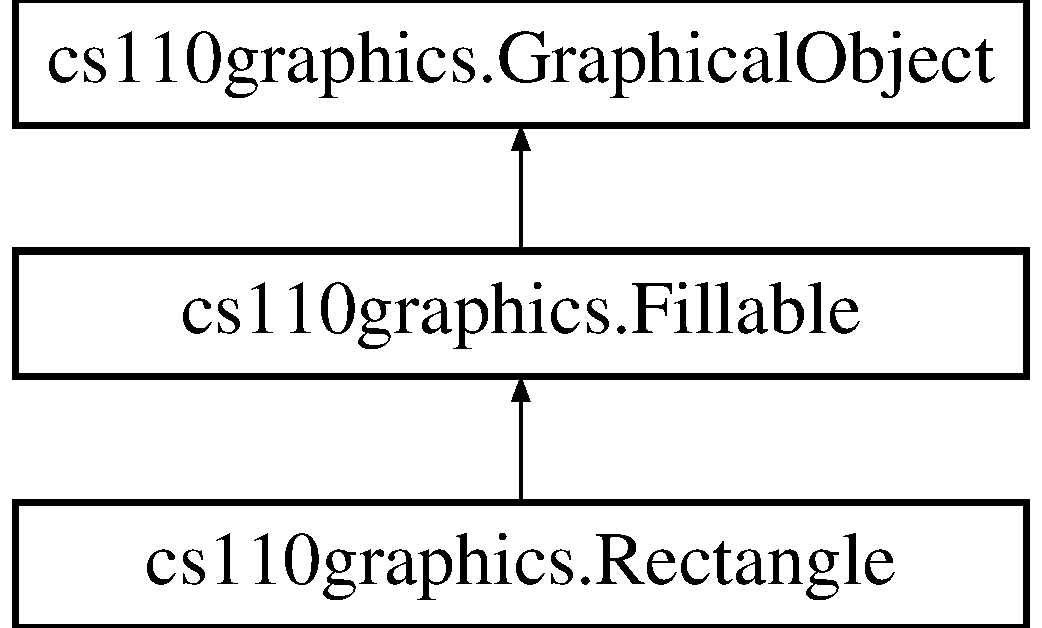
\includegraphics[height=3cm]{classcs110graphics_1_1Rectangle}
\end{center}
\end{figure}
\subsection*{Public Member Functions}
\begin{DoxyCompactItemize}
\item 
def \hyperlink{classcs110graphics_1_1Rectangle_a57049aac9a7f4aa8823112290888a6a8}{\_\-\_\-init\_\-\_\-}
\item 
def \hyperlink{classcs110graphics_1_1Rectangle_a080e6851b24278d7533e0fa9920ea036}{set\_\-side\_\-lengths}
\begin{DoxyCompactList}\small\item\em Sets the width and height of the \hyperlink{classcs110graphics_1_1Rectangle}{Rectangle}. \item\end{DoxyCompactList}\item 
def \hyperlink{classcs110graphics_1_1Fillable_a6772d56158c9fe98a33f01d47cb8aa41}{get\_\-border\_\-color}
\begin{DoxyCompactList}\small\item\em Returns the border color. \item\end{DoxyCompactList}\item 
def \hyperlink{classcs110graphics_1_1Fillable_a6ed7a4288e84a090ec185c8bdff21d0f}{get\_\-border\_\-width}
\begin{DoxyCompactList}\small\item\em Returns the border width. \item\end{DoxyCompactList}\item 
def \hyperlink{classcs110graphics_1_1Fillable_a16c045bc9b63961b696914ee1a1d14d9}{get\_\-fill\_\-color}
\begin{DoxyCompactList}\small\item\em Returns fill color. \item\end{DoxyCompactList}\item 
def \hyperlink{classcs110graphics_1_1Fillable_a514fa0d21297c1372681afae9219fd58}{get\_\-pivot}
\begin{DoxyCompactList}\small\item\em Returns the pivot point. \item\end{DoxyCompactList}\item 
def \hyperlink{classcs110graphics_1_1Fillable_afa6710f6c314de39d19f06d9dd306d7d}{rotate}
\begin{DoxyCompactList}\small\item\em Rotates the object. \item\end{DoxyCompactList}\item 
def \hyperlink{classcs110graphics_1_1Fillable_a80d5b6b6d2ebae867dccecb803075749}{scale}
\begin{DoxyCompactList}\small\item\em Scales the object up or down depending on the factor. \item\end{DoxyCompactList}\item 
def \hyperlink{classcs110graphics_1_1Fillable_a2f830be5d970faac97759910d20d68a4}{set\_\-border\_\-color}
\begin{DoxyCompactList}\small\item\em Sets the border color. \item\end{DoxyCompactList}\item 
def \hyperlink{classcs110graphics_1_1Fillable_a09f05462cb2ed38fdccb244340f05b2b}{set\_\-border\_\-width}
\begin{DoxyCompactList}\small\item\em Sets the border width. \item\end{DoxyCompactList}\item 
def \hyperlink{classcs110graphics_1_1Fillable_a4f24c7186c8d057e42a0209eb1d56be7}{set\_\-fill\_\-color}
\begin{DoxyCompactList}\small\item\em Sets the fill color. \item\end{DoxyCompactList}\item 
def \hyperlink{classcs110graphics_1_1Fillable_a2a6066d1a11c0854ff5ee85e7d9ceb54}{set\_\-pivot}
\begin{DoxyCompactList}\small\item\em Sets the pivot point. \item\end{DoxyCompactList}\item 
def \hyperlink{classcs110graphics_1_1GraphicalObject_adb1af0d5a6baae3f9a08d21a3227c49f}{add\_\-handler}
\begin{DoxyCompactList}\small\item\em Adds a handler to the graphical object. \item\end{DoxyCompactList}\item 
def \hyperlink{classcs110graphics_1_1GraphicalObject_a062789c4cc9de38af32dcc4ff2058607}{get\_\-center}
\begin{DoxyCompactList}\small\item\em Returns the center of the object. \item\end{DoxyCompactList}\item 
def \hyperlink{classcs110graphics_1_1GraphicalObject_a6d9f5718cd0cf249e0d2842971bae17f}{get\_\-depth}
\begin{DoxyCompactList}\small\item\em Returns the depth of the object. \item\end{DoxyCompactList}\item 
def \hyperlink{classcs110graphics_1_1GraphicalObject_aa64d270fb83efa4a54e1a7953512f9cd}{move}
\begin{DoxyCompactList}\small\item\em Moves the object dx pixels horizontally and dy pixels vertically. \item\end{DoxyCompactList}\item 
def \hyperlink{classcs110graphics_1_1GraphicalObject_abe2d480265df7ac9447205c52c6946df}{move\_\-to}
\begin{DoxyCompactList}\small\item\em Moves a graphical object to a point. \item\end{DoxyCompactList}\item 
def \hyperlink{classcs110graphics_1_1GraphicalObject_a20d76d4ee4419c3065d61deb6cbc6700}{set\_\-depth}
\begin{DoxyCompactList}\small\item\em Sets the depth of the \hyperlink{classcs110graphics_1_1GraphicalObject}{GraphicalObject}. \item\end{DoxyCompactList}\end{DoxyCompactItemize}


\subsection{Detailed Description}
A rectangle, which can be added to a \hyperlink{classcs110graphics_1_1Window}{Window} object. 

\subsection{Member Function Documentation}
\hypertarget{classcs110graphics_1_1Rectangle_a57049aac9a7f4aa8823112290888a6a8}{
\index{cs110graphics::Rectangle@{cs110graphics::Rectangle}!\_\-\_\-init\_\-\_\-@{\_\-\_\-init\_\-\_\-}}
\index{\_\-\_\-init\_\-\_\-@{\_\-\_\-init\_\-\_\-}!cs110graphics::Rectangle@{cs110graphics::Rectangle}}
\subsubsection[{\_\-\_\-init\_\-\_\-}]{\setlength{\rightskip}{0pt plus 5cm}def cs110graphics.Rectangle.\_\-\_\-init\_\-\_\- ( {\em self}, \/   {\em window}, \/   {\em width} = {\ttfamily 80}, \/   {\em height} = {\ttfamily 120}, \/   {\em center} = {\ttfamily (200,~200})}}
\label{classcs110graphics_1_1Rectangle_a57049aac9a7f4aa8823112290888a6a8}

\begin{DoxyParams}{Parameters}
\item[{\em window}]-\/ \hyperlink{classcs110graphics_1_1Window}{Window} -\/ the window which the object will be added to \item[{\em width}]-\/ int -\/ {\bfseries (default: 80)} the width of the rectangle \item[{\em height}]-\/ int -\/ {\bfseries (default: 120)} the height of the rectangle \item[{\em center}]-\/ tuple of (int $\ast$ int) -\/ {\bfseries (default: (200, 200))} the center of the rectangle \end{DoxyParams}


Reimplemented from \hyperlink{classcs110graphics_1_1GraphicalObject}{cs110graphics.GraphicalObject}.\hypertarget{classcs110graphics_1_1GraphicalObject_adb1af0d5a6baae3f9a08d21a3227c49f}{
\index{cs110graphics::Rectangle@{cs110graphics::Rectangle}!add\_\-handler@{add\_\-handler}}
\index{add\_\-handler@{add\_\-handler}!cs110graphics::Rectangle@{cs110graphics::Rectangle}}
\subsubsection[{add\_\-handler}]{\setlength{\rightskip}{0pt plus 5cm}def cs110graphics.GraphicalObject.add\_\-handler ( {\em self}, \/   {\em handler\_\-object})\hspace{0.3cm}{\ttfamily  \mbox{[}inherited\mbox{]}}}}
\label{classcs110graphics_1_1GraphicalObject_adb1af0d5a6baae3f9a08d21a3227c49f}


Adds a handler to the graphical object. 
\begin{DoxyParams}{Parameters}
\item[{\em handler\_\-object}]-\/ \hyperlink{classcs110graphics_1_1EventHandler}{EventHandler} -\/ the object that handles the events for this \hyperlink{classcs110graphics_1_1GraphicalObject}{GraphicalObject} \end{DoxyParams}
\hypertarget{classcs110graphics_1_1Fillable_a6772d56158c9fe98a33f01d47cb8aa41}{
\index{cs110graphics::Rectangle@{cs110graphics::Rectangle}!get\_\-border\_\-color@{get\_\-border\_\-color}}
\index{get\_\-border\_\-color@{get\_\-border\_\-color}!cs110graphics::Rectangle@{cs110graphics::Rectangle}}
\subsubsection[{get\_\-border\_\-color}]{\setlength{\rightskip}{0pt plus 5cm}def cs110graphics.Fillable.get\_\-border\_\-color ( {\em self})\hspace{0.3cm}{\ttfamily  \mbox{[}inherited\mbox{]}}}}
\label{classcs110graphics_1_1Fillable_a6772d56158c9fe98a33f01d47cb8aa41}


Returns the border color. \begin{DoxyReturn}{Returns}
border\_\-color -\/ str -\/ Can be either the name of a color (\char`\"{}yellow\char`\"{}), or a hex code (\char`\"{}\#FFFF00\char`\"{}) 
\end{DoxyReturn}
\hypertarget{classcs110graphics_1_1Fillable_a6ed7a4288e84a090ec185c8bdff21d0f}{
\index{cs110graphics::Rectangle@{cs110graphics::Rectangle}!get\_\-border\_\-width@{get\_\-border\_\-width}}
\index{get\_\-border\_\-width@{get\_\-border\_\-width}!cs110graphics::Rectangle@{cs110graphics::Rectangle}}
\subsubsection[{get\_\-border\_\-width}]{\setlength{\rightskip}{0pt plus 5cm}def cs110graphics.Fillable.get\_\-border\_\-width ( {\em self})\hspace{0.3cm}{\ttfamily  \mbox{[}inherited\mbox{]}}}}
\label{classcs110graphics_1_1Fillable_a6ed7a4288e84a090ec185c8bdff21d0f}


Returns the border width. \begin{DoxyReturn}{Returns}
border\_\-width -\/ int 
\end{DoxyReturn}
\hypertarget{classcs110graphics_1_1GraphicalObject_a062789c4cc9de38af32dcc4ff2058607}{
\index{cs110graphics::Rectangle@{cs110graphics::Rectangle}!get\_\-center@{get\_\-center}}
\index{get\_\-center@{get\_\-center}!cs110graphics::Rectangle@{cs110graphics::Rectangle}}
\subsubsection[{get\_\-center}]{\setlength{\rightskip}{0pt plus 5cm}def cs110graphics.GraphicalObject.get\_\-center ( {\em self})\hspace{0.3cm}{\ttfamily  \mbox{[}inherited\mbox{]}}}}
\label{classcs110graphics_1_1GraphicalObject_a062789c4cc9de38af32dcc4ff2058607}


Returns the center of the object. \begin{DoxyReturn}{Returns}
center -\/ tuple 
\end{DoxyReturn}
\hypertarget{classcs110graphics_1_1GraphicalObject_a6d9f5718cd0cf249e0d2842971bae17f}{
\index{cs110graphics::Rectangle@{cs110graphics::Rectangle}!get\_\-depth@{get\_\-depth}}
\index{get\_\-depth@{get\_\-depth}!cs110graphics::Rectangle@{cs110graphics::Rectangle}}
\subsubsection[{get\_\-depth}]{\setlength{\rightskip}{0pt plus 5cm}def cs110graphics.GraphicalObject.get\_\-depth ( {\em self})\hspace{0.3cm}{\ttfamily  \mbox{[}inherited\mbox{]}}}}
\label{classcs110graphics_1_1GraphicalObject_a6d9f5718cd0cf249e0d2842971bae17f}


Returns the depth of the object. \begin{DoxyReturn}{Returns}
depth -\/ int 
\end{DoxyReturn}
\hypertarget{classcs110graphics_1_1Fillable_a16c045bc9b63961b696914ee1a1d14d9}{
\index{cs110graphics::Rectangle@{cs110graphics::Rectangle}!get\_\-fill\_\-color@{get\_\-fill\_\-color}}
\index{get\_\-fill\_\-color@{get\_\-fill\_\-color}!cs110graphics::Rectangle@{cs110graphics::Rectangle}}
\subsubsection[{get\_\-fill\_\-color}]{\setlength{\rightskip}{0pt plus 5cm}def cs110graphics.Fillable.get\_\-fill\_\-color ( {\em self})\hspace{0.3cm}{\ttfamily  \mbox{[}inherited\mbox{]}}}}
\label{classcs110graphics_1_1Fillable_a16c045bc9b63961b696914ee1a1d14d9}


Returns fill color. \begin{DoxyReturn}{Returns}
color -\/ int -\/ Can be either the name of a color (\char`\"{}yellow\char`\"{}), or a hex code (\char`\"{}\#FFFF00\char`\"{}) 
\end{DoxyReturn}
\hypertarget{classcs110graphics_1_1Fillable_a514fa0d21297c1372681afae9219fd58}{
\index{cs110graphics::Rectangle@{cs110graphics::Rectangle}!get\_\-pivot@{get\_\-pivot}}
\index{get\_\-pivot@{get\_\-pivot}!cs110graphics::Rectangle@{cs110graphics::Rectangle}}
\subsubsection[{get\_\-pivot}]{\setlength{\rightskip}{0pt plus 5cm}def cs110graphics.Fillable.get\_\-pivot ( {\em self})\hspace{0.3cm}{\ttfamily  \mbox{[}inherited\mbox{]}}}}
\label{classcs110graphics_1_1Fillable_a514fa0d21297c1372681afae9219fd58}


Returns the pivot point. \begin{DoxyReturn}{Returns}
pivot -\/ tuple (int $\ast$ int) 
\end{DoxyReturn}
\hypertarget{classcs110graphics_1_1GraphicalObject_aa64d270fb83efa4a54e1a7953512f9cd}{
\index{cs110graphics::Rectangle@{cs110graphics::Rectangle}!move@{move}}
\index{move@{move}!cs110graphics::Rectangle@{cs110graphics::Rectangle}}
\subsubsection[{move}]{\setlength{\rightskip}{0pt plus 5cm}def cs110graphics.GraphicalObject.move ( {\em self}, \/   {\em dx}, \/   {\em dy})\hspace{0.3cm}{\ttfamily  \mbox{[}inherited\mbox{]}}}}
\label{classcs110graphics_1_1GraphicalObject_aa64d270fb83efa4a54e1a7953512f9cd}


Moves the object dx pixels horizontally and dy pixels vertically. 
\begin{DoxyParams}{Parameters}
\item[{\em dx}]-\/ int \item[{\em dy}]-\/ int \end{DoxyParams}
\hypertarget{classcs110graphics_1_1GraphicalObject_abe2d480265df7ac9447205c52c6946df}{
\index{cs110graphics::Rectangle@{cs110graphics::Rectangle}!move\_\-to@{move\_\-to}}
\index{move\_\-to@{move\_\-to}!cs110graphics::Rectangle@{cs110graphics::Rectangle}}
\subsubsection[{move\_\-to}]{\setlength{\rightskip}{0pt plus 5cm}def cs110graphics.GraphicalObject.move\_\-to ( {\em self}, \/   {\em point})\hspace{0.3cm}{\ttfamily  \mbox{[}inherited\mbox{]}}}}
\label{classcs110graphics_1_1GraphicalObject_abe2d480265df7ac9447205c52c6946df}


Moves a graphical object to a point. 
\begin{DoxyParams}{Parameters}
\item[{\em point}]-\/ tuple of (int $\ast$ int) \end{DoxyParams}
\hypertarget{classcs110graphics_1_1Fillable_afa6710f6c314de39d19f06d9dd306d7d}{
\index{cs110graphics::Rectangle@{cs110graphics::Rectangle}!rotate@{rotate}}
\index{rotate@{rotate}!cs110graphics::Rectangle@{cs110graphics::Rectangle}}
\subsubsection[{rotate}]{\setlength{\rightskip}{0pt plus 5cm}def cs110graphics.Fillable.rotate ( {\em self}, \/   {\em degrees})\hspace{0.3cm}{\ttfamily  \mbox{[}inherited\mbox{]}}}}
\label{classcs110graphics_1_1Fillable_afa6710f6c314de39d19f06d9dd306d7d}


Rotates the object. 
\begin{DoxyParams}{Parameters}
\item[{\em degrees}]-\/ int \end{DoxyParams}


Reimplemented in \hyperlink{classcs110graphics_1_1Circle_a0532651c10c084766ac3032c57107eb0}{cs110graphics.Circle}, and \hyperlink{classcs110graphics_1_1Oval_a98bb8103f19d2df5a875db6943fde6e2}{cs110graphics.Oval}.\hypertarget{classcs110graphics_1_1Fillable_a80d5b6b6d2ebae867dccecb803075749}{
\index{cs110graphics::Rectangle@{cs110graphics::Rectangle}!scale@{scale}}
\index{scale@{scale}!cs110graphics::Rectangle@{cs110graphics::Rectangle}}
\subsubsection[{scale}]{\setlength{\rightskip}{0pt plus 5cm}def cs110graphics.Fillable.scale ( {\em self}, \/   {\em factor})\hspace{0.3cm}{\ttfamily  \mbox{[}inherited\mbox{]}}}}
\label{classcs110graphics_1_1Fillable_a80d5b6b6d2ebae867dccecb803075749}


Scales the object up or down depending on the factor. 
\begin{DoxyParams}{Parameters}
\item[{\em factor}]-\/ float \end{DoxyParams}


Reimplemented in \hyperlink{classcs110graphics_1_1Circle_a9ffed9eb3f191fafadd5b2d7e7735c18}{cs110graphics.Circle}, and \hyperlink{classcs110graphics_1_1Oval_accf5ef95d1127e0abe9f09823051d75f}{cs110graphics.Oval}.\hypertarget{classcs110graphics_1_1Fillable_a2f830be5d970faac97759910d20d68a4}{
\index{cs110graphics::Rectangle@{cs110graphics::Rectangle}!set\_\-border\_\-color@{set\_\-border\_\-color}}
\index{set\_\-border\_\-color@{set\_\-border\_\-color}!cs110graphics::Rectangle@{cs110graphics::Rectangle}}
\subsubsection[{set\_\-border\_\-color}]{\setlength{\rightskip}{0pt plus 5cm}def cs110graphics.Fillable.set\_\-border\_\-color ( {\em self}, \/   {\em color})\hspace{0.3cm}{\ttfamily  \mbox{[}inherited\mbox{]}}}}
\label{classcs110graphics_1_1Fillable_a2f830be5d970faac97759910d20d68a4}


Sets the border color. 
\begin{DoxyParams}{Parameters}
\item[{\em color}]-\/ string -\/ Can be either the name of a color (\char`\"{}yellow\char`\"{}), or a hex code (\char`\"{}\#FFFF00\char`\"{}) \end{DoxyParams}
\hypertarget{classcs110graphics_1_1Fillable_a09f05462cb2ed38fdccb244340f05b2b}{
\index{cs110graphics::Rectangle@{cs110graphics::Rectangle}!set\_\-border\_\-width@{set\_\-border\_\-width}}
\index{set\_\-border\_\-width@{set\_\-border\_\-width}!cs110graphics::Rectangle@{cs110graphics::Rectangle}}
\subsubsection[{set\_\-border\_\-width}]{\setlength{\rightskip}{0pt plus 5cm}def cs110graphics.Fillable.set\_\-border\_\-width ( {\em self}, \/   {\em width})\hspace{0.3cm}{\ttfamily  \mbox{[}inherited\mbox{]}}}}
\label{classcs110graphics_1_1Fillable_a09f05462cb2ed38fdccb244340f05b2b}


Sets the border width. 
\begin{DoxyParams}{Parameters}
\item[{\em width}]-\/ int \end{DoxyParams}
\hypertarget{classcs110graphics_1_1GraphicalObject_a20d76d4ee4419c3065d61deb6cbc6700}{
\index{cs110graphics::Rectangle@{cs110graphics::Rectangle}!set\_\-depth@{set\_\-depth}}
\index{set\_\-depth@{set\_\-depth}!cs110graphics::Rectangle@{cs110graphics::Rectangle}}
\subsubsection[{set\_\-depth}]{\setlength{\rightskip}{0pt plus 5cm}def cs110graphics.GraphicalObject.set\_\-depth ( {\em self}, \/   {\em depth})\hspace{0.3cm}{\ttfamily  \mbox{[}inherited\mbox{]}}}}
\label{classcs110graphics_1_1GraphicalObject_a20d76d4ee4419c3065d61deb6cbc6700}


Sets the depth of the \hyperlink{classcs110graphics_1_1GraphicalObject}{GraphicalObject}. 
\begin{DoxyParams}{Parameters}
\item[{\em depth}]-\/ int \end{DoxyParams}
\hypertarget{classcs110graphics_1_1Fillable_a4f24c7186c8d057e42a0209eb1d56be7}{
\index{cs110graphics::Rectangle@{cs110graphics::Rectangle}!set\_\-fill\_\-color@{set\_\-fill\_\-color}}
\index{set\_\-fill\_\-color@{set\_\-fill\_\-color}!cs110graphics::Rectangle@{cs110graphics::Rectangle}}
\subsubsection[{set\_\-fill\_\-color}]{\setlength{\rightskip}{0pt plus 5cm}def cs110graphics.Fillable.set\_\-fill\_\-color ( {\em self}, \/   {\em color})\hspace{0.3cm}{\ttfamily  \mbox{[}inherited\mbox{]}}}}
\label{classcs110graphics_1_1Fillable_a4f24c7186c8d057e42a0209eb1d56be7}


Sets the fill color. 
\begin{DoxyParams}{Parameters}
\item[{\em color}]-\/ string -\/ Can be either the name of a color (\char`\"{}yellow\char`\"{}), or a hex code (\char`\"{}\#FFFF00\char`\"{}) \end{DoxyParams}
\hypertarget{classcs110graphics_1_1Fillable_a2a6066d1a11c0854ff5ee85e7d9ceb54}{
\index{cs110graphics::Rectangle@{cs110graphics::Rectangle}!set\_\-pivot@{set\_\-pivot}}
\index{set\_\-pivot@{set\_\-pivot}!cs110graphics::Rectangle@{cs110graphics::Rectangle}}
\subsubsection[{set\_\-pivot}]{\setlength{\rightskip}{0pt plus 5cm}def cs110graphics.Fillable.set\_\-pivot ( {\em self}, \/   {\em pivot})\hspace{0.3cm}{\ttfamily  \mbox{[}inherited\mbox{]}}}}
\label{classcs110graphics_1_1Fillable_a2a6066d1a11c0854ff5ee85e7d9ceb54}


Sets the pivot point. 
\begin{DoxyParams}{Parameters}
\item[{\em pivot}]-\/ tuple of (int $\ast$ int) \end{DoxyParams}
\hypertarget{classcs110graphics_1_1Rectangle_a080e6851b24278d7533e0fa9920ea036}{
\index{cs110graphics::Rectangle@{cs110graphics::Rectangle}!set\_\-side\_\-lengths@{set\_\-side\_\-lengths}}
\index{set\_\-side\_\-lengths@{set\_\-side\_\-lengths}!cs110graphics::Rectangle@{cs110graphics::Rectangle}}
\subsubsection[{set\_\-side\_\-lengths}]{\setlength{\rightskip}{0pt plus 5cm}def cs110graphics.Rectangle.set\_\-side\_\-lengths ( {\em self}, \/   {\em width}, \/   {\em height})}}
\label{classcs110graphics_1_1Rectangle_a080e6851b24278d7533e0fa9920ea036}


Sets the width and height of the \hyperlink{classcs110graphics_1_1Rectangle}{Rectangle}. 
\begin{DoxyParams}{Parameters}
\item[{\em width}]-\/ int \item[{\em height}]-\/ int \end{DoxyParams}


The documentation for this class was generated from the following file:\begin{DoxyCompactItemize}
\item 
\hyperlink{cs110graphics_8py}{cs110graphics.py}\end{DoxyCompactItemize}

\hypertarget{classsample_1_1Remover}{
\section{sample.Remover Class Reference}
\label{classsample_1_1Remover}\index{sample::Remover@{sample::Remover}}
}
Inheritance diagram for sample.Remover::\begin{figure}[H]
\begin{center}
\leavevmode
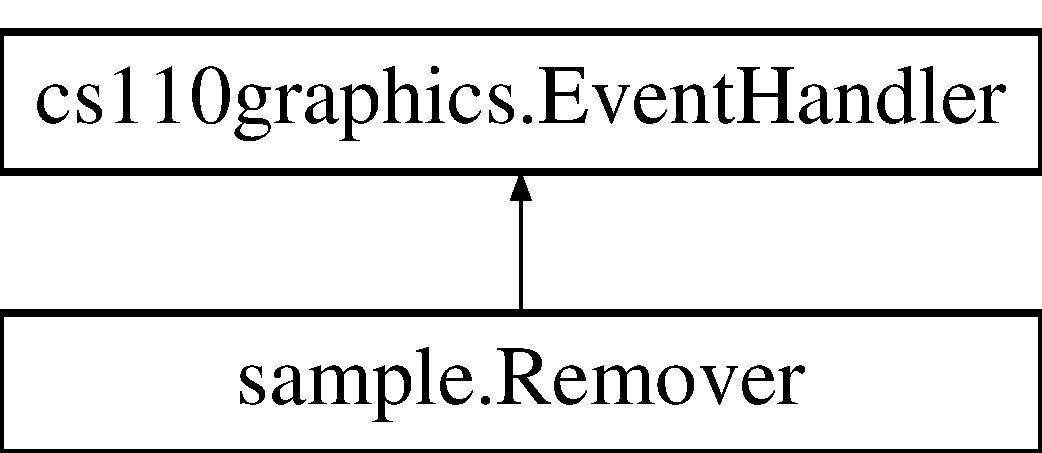
\includegraphics[height=2cm]{classsample_1_1Remover}
\end{center}
\end{figure}
\subsection*{Public Member Functions}
\begin{DoxyCompactItemize}
\item 
def \hyperlink{classsample_1_1Remover_a84484de500f08402e582c126432e0cf1}{handle\_\-mouse\_\-release}
\begin{DoxyCompactList}\small\item\em Handles a mouse release. \item\end{DoxyCompactList}\item 
def \hyperlink{classcs110graphics_1_1EventHandler_af3fb3531d0b23f1430a830586cd07906}{handle\_\-key\_\-press}
\begin{DoxyCompactList}\small\item\em Handles a key press. \item\end{DoxyCompactList}\item 
def \hyperlink{classcs110graphics_1_1EventHandler_a2849f60251baa44252992162521f2473}{handle\_\-key\_\-release}
\begin{DoxyCompactList}\small\item\em Handles a key release. \item\end{DoxyCompactList}\item 
def \hyperlink{classcs110graphics_1_1EventHandler_a13af3268f8a1aa36b8483eb2deffef15}{handle\_\-mouse\_\-enter}
\begin{DoxyCompactList}\small\item\em Handles when a mouse enters an object. \item\end{DoxyCompactList}\item 
def \hyperlink{classcs110graphics_1_1EventHandler_a5deaf2b6b8055e97ac0ddf6603132c64}{handle\_\-mouse\_\-leave}
\begin{DoxyCompactList}\small\item\em Handles when a mouse leaves an object. \item\end{DoxyCompactList}\item 
def \hyperlink{classcs110graphics_1_1EventHandler_a521fdcd170d15c0b8baa124c78b6d1ef}{handle\_\-mouse\_\-move}
\begin{DoxyCompactList}\small\item\em Handles a mouse move. \item\end{DoxyCompactList}\item 
def \hyperlink{classcs110graphics_1_1EventHandler_a547873123ebcd3fcc63a2e03d2a2fee3}{handle\_\-mouse\_\-press}
\begin{DoxyCompactList}\small\item\em Handles a mouse press. \item\end{DoxyCompactList}\end{DoxyCompactItemize}


\subsection{Member Function Documentation}
\hypertarget{classcs110graphics_1_1EventHandler_af3fb3531d0b23f1430a830586cd07906}{
\index{sample::Remover@{sample::Remover}!handle\_\-key\_\-press@{handle\_\-key\_\-press}}
\index{handle\_\-key\_\-press@{handle\_\-key\_\-press}!sample::Remover@{sample::Remover}}
\subsubsection[{handle\_\-key\_\-press}]{\setlength{\rightskip}{0pt plus 5cm}def cs110graphics.EventHandler.handle\_\-key\_\-press ( {\em self}, \/   {\em event})\hspace{0.3cm}{\ttfamily  \mbox{[}inherited\mbox{]}}}}
\label{classcs110graphics_1_1EventHandler_af3fb3531d0b23f1430a830586cd07906}


Handles a key press. This function will be called whenever a key is pressed while the window is active. The event parameter can be used to determine which key was pressed. For example: 
\begin{DoxyCode}
 class Handler(EventHandler):
     def handle_key_press(self, event):
         if "a" == event.get_key():
             # do something when a is pressed...
         else:
             # do something else...
\end{DoxyCode}
 
\begin{DoxyParams}{Parameters}
\item[{\em event}]-\/ \hyperlink{classcs110graphics_1_1Event}{Event} -\/ the event that occurred \end{DoxyParams}


Reimplemented in \hyperlink{classtest_1_1Handler_a3d418670cfafce344b8b7155b4df438e}{test.Handler}, \hyperlink{classtest_1_1Bot_a23b90152ec8fa124851cd5fe6944beed}{test.Bot}, and \hyperlink{classtext__move_1_1Handler_a5a42b4eb6df32fce14be58a45a7a82f0}{text\_\-move.Handler}.\hypertarget{classcs110graphics_1_1EventHandler_a2849f60251baa44252992162521f2473}{
\index{sample::Remover@{sample::Remover}!handle\_\-key\_\-release@{handle\_\-key\_\-release}}
\index{handle\_\-key\_\-release@{handle\_\-key\_\-release}!sample::Remover@{sample::Remover}}
\subsubsection[{handle\_\-key\_\-release}]{\setlength{\rightskip}{0pt plus 5cm}def cs110graphics.EventHandler.handle\_\-key\_\-release ( {\em self}, \/   {\em event})\hspace{0.3cm}{\ttfamily  \mbox{[}inherited\mbox{]}}}}
\label{classcs110graphics_1_1EventHandler_a2849f60251baa44252992162521f2473}


Handles a key release. This method will be called whenever a key is released while the window is active. The event parameter can be used to determine which key was pressed. For example: 
\begin{DoxyCode}
 class Handler(EventHandler):
     def handle_key_release(self, event):
         if "a" == event.get_key():
             # do something when a is released...
         else:
             # do something else...
\end{DoxyCode}
 
\begin{DoxyParams}{Parameters}
\item[{\em event}]-\/ \hyperlink{classcs110graphics_1_1Event}{Event} -\/ the event that occurred \end{DoxyParams}


Reimplemented in \hyperlink{classtest_1_1Bot_a173d0fff530e0987193e9006b24f218b}{test.Bot}.\hypertarget{classcs110graphics_1_1EventHandler_a13af3268f8a1aa36b8483eb2deffef15}{
\index{sample::Remover@{sample::Remover}!handle\_\-mouse\_\-enter@{handle\_\-mouse\_\-enter}}
\index{handle\_\-mouse\_\-enter@{handle\_\-mouse\_\-enter}!sample::Remover@{sample::Remover}}
\subsubsection[{handle\_\-mouse\_\-enter}]{\setlength{\rightskip}{0pt plus 5cm}def cs110graphics.EventHandler.handle\_\-mouse\_\-enter ( {\em self}, \/   {\em event})\hspace{0.3cm}{\ttfamily  \mbox{[}inherited\mbox{]}}}}
\label{classcs110graphics_1_1EventHandler_a13af3268f8a1aa36b8483eb2deffef15}


Handles when a mouse enters an object. \begin{Desc}
\item[\hyperlink{bug__bug000001}{Bug}]Overrides of this method is likely to be called more often than expected and many \hyperlink{classcs110graphics_1_1GraphicalObject}{GraphicalObject} methods will not work correctly with when called within the method, avoid using this if possible.\end{Desc}
This is called by the system when the mouse enters the \hyperlink{classcs110graphics_1_1GraphicalObject}{GraphicalObject} that this handler is an event handler for. The event parameter can be used to determine the location at which the mouse entered the object. 
\begin{DoxyCode}
 class Handler(EventHandler):
     def handle_mouse_enter(self, event):
         mouse_location = event.get_mouse_location()
\end{DoxyCode}
 
\begin{DoxyParams}{Parameters}
\item[{\em event}]-\/ \hyperlink{classcs110graphics_1_1Event}{Event} -\/ the event that occurred \end{DoxyParams}


Reimplemented in \hyperlink{classtest_1_1Bot_a0b184ab86d0dd6121e55394a24c8751e}{test.Bot}, and \hyperlink{classtext__move_1_1Handler_a51652a1d51554e661117de1ee7856169}{text\_\-move.Handler}.\hypertarget{classcs110graphics_1_1EventHandler_a5deaf2b6b8055e97ac0ddf6603132c64}{
\index{sample::Remover@{sample::Remover}!handle\_\-mouse\_\-leave@{handle\_\-mouse\_\-leave}}
\index{handle\_\-mouse\_\-leave@{handle\_\-mouse\_\-leave}!sample::Remover@{sample::Remover}}
\subsubsection[{handle\_\-mouse\_\-leave}]{\setlength{\rightskip}{0pt plus 5cm}def cs110graphics.EventHandler.handle\_\-mouse\_\-leave ( {\em self}, \/   {\em event})\hspace{0.3cm}{\ttfamily  \mbox{[}inherited\mbox{]}}}}
\label{classcs110graphics_1_1EventHandler_a5deaf2b6b8055e97ac0ddf6603132c64}


Handles when a mouse leaves an object. This is called by the system when the mouse leaves the \hyperlink{classcs110graphics_1_1GraphicalObject}{GraphicalObject} that this handler is an event handler for. The event parameter can be used to determine the location at which the mouse left the object. 
\begin{DoxyCode}
 class Handler(EventHandler):
     def handle_mouse_leave(self, event):
         mouse_location = event.get_mouse_location()
\end{DoxyCode}
 
\begin{DoxyParams}{Parameters}
\item[{\em event}]-\/ \hyperlink{classcs110graphics_1_1Event}{Event} -\/ the event that occurred \end{DoxyParams}


Reimplemented in \hyperlink{classtest_1_1Bot_a2b65e6ecaba1afb4f117b74a684b4387}{test.Bot}.\hypertarget{classcs110graphics_1_1EventHandler_a521fdcd170d15c0b8baa124c78b6d1ef}{
\index{sample::Remover@{sample::Remover}!handle\_\-mouse\_\-move@{handle\_\-mouse\_\-move}}
\index{handle\_\-mouse\_\-move@{handle\_\-mouse\_\-move}!sample::Remover@{sample::Remover}}
\subsubsection[{handle\_\-mouse\_\-move}]{\setlength{\rightskip}{0pt plus 5cm}def cs110graphics.EventHandler.handle\_\-mouse\_\-move ( {\em self}, \/   {\em event})\hspace{0.3cm}{\ttfamily  \mbox{[}inherited\mbox{]}}}}
\label{classcs110graphics_1_1EventHandler_a521fdcd170d15c0b8baa124c78b6d1ef}


Handles a mouse move. This is called by the system when the mouse moves within the \hyperlink{classcs110graphics_1_1GraphicalObject}{GraphicalObject} that this handler is an event handler for. The event parameter can be used to determine the location that the mouse moved to. 
\begin{DoxyCode}
 class Handler(EventHandler):
     def handle_mouse_move(self, event):
         mouse_location = event.get_mouse_location()
\end{DoxyCode}
 
\begin{DoxyParams}{Parameters}
\item[{\em event}]-\/ \hyperlink{classcs110graphics_1_1Event}{Event} -\/ the event that occurred \end{DoxyParams}


Reimplemented in \hyperlink{classtest_1_1Handler_a88a2d58962eb4bf7338332848fa5fc3a}{test.Handler}, and \hyperlink{classtest_1_1Bot_ad1464516fb04013fa7e353a78f0ec218}{test.Bot}.\hypertarget{classcs110graphics_1_1EventHandler_a547873123ebcd3fcc63a2e03d2a2fee3}{
\index{sample::Remover@{sample::Remover}!handle\_\-mouse\_\-press@{handle\_\-mouse\_\-press}}
\index{handle\_\-mouse\_\-press@{handle\_\-mouse\_\-press}!sample::Remover@{sample::Remover}}
\subsubsection[{handle\_\-mouse\_\-press}]{\setlength{\rightskip}{0pt plus 5cm}def cs110graphics.EventHandler.handle\_\-mouse\_\-press ( {\em self}, \/   {\em event})\hspace{0.3cm}{\ttfamily  \mbox{[}inherited\mbox{]}}}}
\label{classcs110graphics_1_1EventHandler_a547873123ebcd3fcc63a2e03d2a2fee3}


Handles a mouse press. This is called by the system when a mouse button is pressed while the mouse is on the \hyperlink{classcs110graphics_1_1GraphicalObject}{GraphicalObject} that this handler is an event handler for. The event parameter can be used to determine the location at which the mouse button was pressed and which mouse button was pressed. 
\begin{DoxyCode}
 class Handler(EventHandler):
     def handle_mouse_press(self, event):
         mouse_location = event.get_mouse_location()
         mouse_button = event.get_button()
\end{DoxyCode}
 
\begin{DoxyParams}{Parameters}
\item[{\em event}]-\/ \hyperlink{classcs110graphics_1_1Event}{Event} -\/ the event that occurred \end{DoxyParams}


Reimplemented in \hyperlink{classtest_1_1Bot_a970422a4391cc2b9ff89a2e42063bb6e}{test.Bot}, and \hyperlink{classtext__move_1_1H2_a13611a7fe23eefc92b40ff3874e026bd}{text\_\-move.H2}.\hypertarget{classsample_1_1Remover_a84484de500f08402e582c126432e0cf1}{
\index{sample::Remover@{sample::Remover}!handle\_\-mouse\_\-release@{handle\_\-mouse\_\-release}}
\index{handle\_\-mouse\_\-release@{handle\_\-mouse\_\-release}!sample::Remover@{sample::Remover}}
\subsubsection[{handle\_\-mouse\_\-release}]{\setlength{\rightskip}{0pt plus 5cm}def sample.Remover.handle\_\-mouse\_\-release ( {\em self}, \/   {\em event})}}
\label{classsample_1_1Remover_a84484de500f08402e582c126432e0cf1}


Handles a mouse release. This is called by the system when a mouse button is released while the mouse is on the GraphicalObject that this handler is an event handler for. The event parameter can be used to determine the location at which the mouse button was released and which mouse button was released. 
\begin{DoxyCode}
 class Handler(EventHandler):
     def handle_mouse_release(self, event):
         mouse_location = event.get_mouse_location()
         mouse_button = event.get_button()
\end{DoxyCode}
 
\begin{DoxyParams}{Parameters}
\item[{\em event}]-\/ Event -\/ the event that occurred \end{DoxyParams}


Reimplemented from \hyperlink{classcs110graphics_1_1EventHandler_a320a7dbf68d37e0101b237bff1713088}{cs110graphics.EventHandler}.

The documentation for this class was generated from the following file:\begin{DoxyCompactItemize}
\item 
sample.py\end{DoxyCompactItemize}

\hypertarget{classcs110graphics_1_1Square}{
\section{cs110graphics.Square Class Reference}
\label{classcs110graphics_1_1Square}\index{cs110graphics::Square@{cs110graphics::Square}}
}


A square, which can be added to a \hyperlink{classcs110graphics_1_1Window}{Window} object.  
Inheritance diagram for cs110graphics.Square::\begin{figure}[H]
\begin{center}
\leavevmode
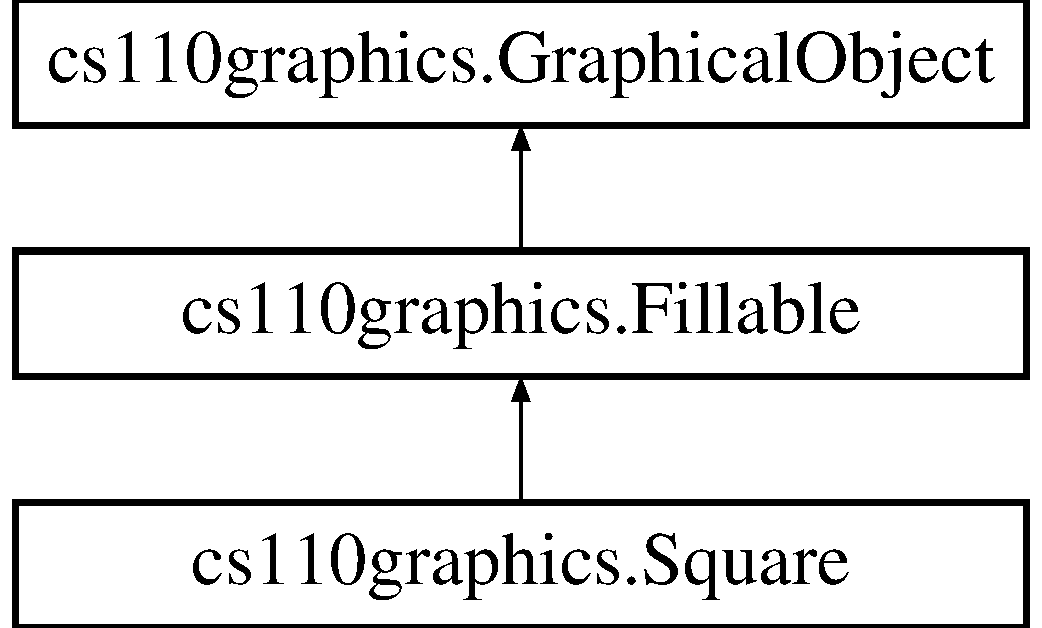
\includegraphics[height=3cm]{classcs110graphics_1_1Square}
\end{center}
\end{figure}
\subsection*{Public Member Functions}
\begin{DoxyCompactItemize}
\item 
def \hyperlink{classcs110graphics_1_1Square_ae4b847029070a73478fd7dd2eefeb58e}{\_\-\_\-init\_\-\_\-}
\item 
def \hyperlink{classcs110graphics_1_1Square_a4b650f9ef28d4fab88d36ce65e8e0cf1}{set\_\-side\_\-length}
\begin{DoxyCompactList}\small\item\em Sets the side length of the \hyperlink{classcs110graphics_1_1Square}{Square}. \item\end{DoxyCompactList}\item 
def \hyperlink{classcs110graphics_1_1Fillable_a6772d56158c9fe98a33f01d47cb8aa41}{get\_\-border\_\-color}
\begin{DoxyCompactList}\small\item\em Returns the border color. \item\end{DoxyCompactList}\item 
def \hyperlink{classcs110graphics_1_1Fillable_a6ed7a4288e84a090ec185c8bdff21d0f}{get\_\-border\_\-width}
\begin{DoxyCompactList}\small\item\em Returns the border width. \item\end{DoxyCompactList}\item 
def \hyperlink{classcs110graphics_1_1Fillable_a16c045bc9b63961b696914ee1a1d14d9}{get\_\-fill\_\-color}
\begin{DoxyCompactList}\small\item\em Returns fill color. \item\end{DoxyCompactList}\item 
def \hyperlink{classcs110graphics_1_1Fillable_a514fa0d21297c1372681afae9219fd58}{get\_\-pivot}
\begin{DoxyCompactList}\small\item\em Returns the pivot point. \item\end{DoxyCompactList}\item 
def \hyperlink{classcs110graphics_1_1Fillable_afa6710f6c314de39d19f06d9dd306d7d}{rotate}
\begin{DoxyCompactList}\small\item\em Rotates the object. \item\end{DoxyCompactList}\item 
def \hyperlink{classcs110graphics_1_1Fillable_a80d5b6b6d2ebae867dccecb803075749}{scale}
\begin{DoxyCompactList}\small\item\em Scales the object up or down depending on the factor. \item\end{DoxyCompactList}\item 
def \hyperlink{classcs110graphics_1_1Fillable_ae8f6c476e29c0810453dc16948e1730c}{move}
\begin{DoxyCompactList}\small\item\em Moves the object dx pixels horizontally and dy pixels vertically. \item\end{DoxyCompactList}\item 
def \hyperlink{classcs110graphics_1_1Fillable_adcabc14e76d1160ff591b9ef7f3d6a97}{move\_\-to}
\begin{DoxyCompactList}\small\item\em Moves a graphical object to a point. \item\end{DoxyCompactList}\item 
def \hyperlink{classcs110graphics_1_1Fillable_a2f830be5d970faac97759910d20d68a4}{set\_\-border\_\-color}
\begin{DoxyCompactList}\small\item\em Sets the border color. \item\end{DoxyCompactList}\item 
def \hyperlink{classcs110graphics_1_1Fillable_a09f05462cb2ed38fdccb244340f05b2b}{set\_\-border\_\-width}
\begin{DoxyCompactList}\small\item\em Sets the border width. \item\end{DoxyCompactList}\item 
def \hyperlink{classcs110graphics_1_1Fillable_a4f24c7186c8d057e42a0209eb1d56be7}{set\_\-fill\_\-color}
\begin{DoxyCompactList}\small\item\em Sets the fill color. \item\end{DoxyCompactList}\item 
def \hyperlink{classcs110graphics_1_1Fillable_a2a6066d1a11c0854ff5ee85e7d9ceb54}{set\_\-pivot}
\begin{DoxyCompactList}\small\item\em Sets the pivot point. \item\end{DoxyCompactList}\item 
def \hyperlink{classcs110graphics_1_1GraphicalObject_adb1af0d5a6baae3f9a08d21a3227c49f}{add\_\-handler}
\begin{DoxyCompactList}\small\item\em Adds a handler to the graphical object. \item\end{DoxyCompactList}\item 
def \hyperlink{classcs110graphics_1_1GraphicalObject_a062789c4cc9de38af32dcc4ff2058607}{get\_\-center}
\begin{DoxyCompactList}\small\item\em Returns the center of the object. \item\end{DoxyCompactList}\item 
def \hyperlink{classcs110graphics_1_1GraphicalObject_a6d9f5718cd0cf249e0d2842971bae17f}{get\_\-depth}
\begin{DoxyCompactList}\small\item\em Returns the depth of the object. \item\end{DoxyCompactList}\item 
def \hyperlink{classcs110graphics_1_1GraphicalObject_a20d76d4ee4419c3065d61deb6cbc6700}{set\_\-depth}
\begin{DoxyCompactList}\small\item\em Sets the depth of the \hyperlink{classcs110graphics_1_1GraphicalObject}{GraphicalObject}. \item\end{DoxyCompactList}\end{DoxyCompactItemize}


\subsection{Detailed Description}
A square, which can be added to a \hyperlink{classcs110graphics_1_1Window}{Window} object. 

\subsection{Member Function Documentation}
\hypertarget{classcs110graphics_1_1Square_ae4b847029070a73478fd7dd2eefeb58e}{
\index{cs110graphics::Square@{cs110graphics::Square}!\_\-\_\-init\_\-\_\-@{\_\-\_\-init\_\-\_\-}}
\index{\_\-\_\-init\_\-\_\-@{\_\-\_\-init\_\-\_\-}!cs110graphics::Square@{cs110graphics::Square}}
\subsubsection[{\_\-\_\-init\_\-\_\-}]{\setlength{\rightskip}{0pt plus 5cm}def cs110graphics.Square.\_\-\_\-init\_\-\_\- ( {\em self}, \/   {\em window}, \/   {\em side\_\-length} = {\ttfamily 80}, \/   {\em center} = {\ttfamily (200,~200})}}
\label{classcs110graphics_1_1Square_ae4b847029070a73478fd7dd2eefeb58e}

\begin{DoxyParams}{Parameters}
\item[{\em window}]-\/ \hyperlink{classcs110graphics_1_1Window}{Window} -\/ the window which the object will be added to \item[{\em side\_\-length}]-\/ int -\/ {\bfseries (default: 40)} the side length \item[{\em center}]-\/ tuple of (int $\ast$ int) -\/ {\bfseries (default: (200, 200))} the center of the square \end{DoxyParams}
\hypertarget{classcs110graphics_1_1GraphicalObject_adb1af0d5a6baae3f9a08d21a3227c49f}{
\index{cs110graphics::Square@{cs110graphics::Square}!add\_\-handler@{add\_\-handler}}
\index{add\_\-handler@{add\_\-handler}!cs110graphics::Square@{cs110graphics::Square}}
\subsubsection[{add\_\-handler}]{\setlength{\rightskip}{0pt plus 5cm}def cs110graphics.GraphicalObject.add\_\-handler ( {\em self}, \/   {\em handler\_\-object})\hspace{0.3cm}{\ttfamily  \mbox{[}inherited\mbox{]}}}}
\label{classcs110graphics_1_1GraphicalObject_adb1af0d5a6baae3f9a08d21a3227c49f}


Adds a handler to the graphical object. 
\begin{DoxyParams}{Parameters}
\item[{\em handler\_\-object}]-\/ \hyperlink{classcs110graphics_1_1EventHandler}{EventHandler} -\/ the object that handles the events for this \hyperlink{classcs110graphics_1_1GraphicalObject}{GraphicalObject} \end{DoxyParams}
\hypertarget{classcs110graphics_1_1Fillable_a6772d56158c9fe98a33f01d47cb8aa41}{
\index{cs110graphics::Square@{cs110graphics::Square}!get\_\-border\_\-color@{get\_\-border\_\-color}}
\index{get\_\-border\_\-color@{get\_\-border\_\-color}!cs110graphics::Square@{cs110graphics::Square}}
\subsubsection[{get\_\-border\_\-color}]{\setlength{\rightskip}{0pt plus 5cm}def cs110graphics.Fillable.get\_\-border\_\-color ( {\em self})\hspace{0.3cm}{\ttfamily  \mbox{[}inherited\mbox{]}}}}
\label{classcs110graphics_1_1Fillable_a6772d56158c9fe98a33f01d47cb8aa41}


Returns the border color. \begin{DoxyReturn}{Returns}
border\_\-color -\/ str -\/ Can be either the name of a color (\char`\"{}yellow\char`\"{}), or a hex code (\char`\"{}\#FFFF00\char`\"{}) 
\end{DoxyReturn}
\hypertarget{classcs110graphics_1_1Fillable_a6ed7a4288e84a090ec185c8bdff21d0f}{
\index{cs110graphics::Square@{cs110graphics::Square}!get\_\-border\_\-width@{get\_\-border\_\-width}}
\index{get\_\-border\_\-width@{get\_\-border\_\-width}!cs110graphics::Square@{cs110graphics::Square}}
\subsubsection[{get\_\-border\_\-width}]{\setlength{\rightskip}{0pt plus 5cm}def cs110graphics.Fillable.get\_\-border\_\-width ( {\em self})\hspace{0.3cm}{\ttfamily  \mbox{[}inherited\mbox{]}}}}
\label{classcs110graphics_1_1Fillable_a6ed7a4288e84a090ec185c8bdff21d0f}


Returns the border width. \begin{DoxyReturn}{Returns}
border\_\-width -\/ int 
\end{DoxyReturn}
\hypertarget{classcs110graphics_1_1GraphicalObject_a062789c4cc9de38af32dcc4ff2058607}{
\index{cs110graphics::Square@{cs110graphics::Square}!get\_\-center@{get\_\-center}}
\index{get\_\-center@{get\_\-center}!cs110graphics::Square@{cs110graphics::Square}}
\subsubsection[{get\_\-center}]{\setlength{\rightskip}{0pt plus 5cm}def cs110graphics.GraphicalObject.get\_\-center ( {\em self})\hspace{0.3cm}{\ttfamily  \mbox{[}inherited\mbox{]}}}}
\label{classcs110graphics_1_1GraphicalObject_a062789c4cc9de38af32dcc4ff2058607}


Returns the center of the object. \begin{DoxyReturn}{Returns}
center -\/ tuple 
\end{DoxyReturn}
\hypertarget{classcs110graphics_1_1GraphicalObject_a6d9f5718cd0cf249e0d2842971bae17f}{
\index{cs110graphics::Square@{cs110graphics::Square}!get\_\-depth@{get\_\-depth}}
\index{get\_\-depth@{get\_\-depth}!cs110graphics::Square@{cs110graphics::Square}}
\subsubsection[{get\_\-depth}]{\setlength{\rightskip}{0pt plus 5cm}def cs110graphics.GraphicalObject.get\_\-depth ( {\em self})\hspace{0.3cm}{\ttfamily  \mbox{[}inherited\mbox{]}}}}
\label{classcs110graphics_1_1GraphicalObject_a6d9f5718cd0cf249e0d2842971bae17f}


Returns the depth of the object. \begin{DoxyReturn}{Returns}
depth -\/ int 
\end{DoxyReturn}
\hypertarget{classcs110graphics_1_1Fillable_a16c045bc9b63961b696914ee1a1d14d9}{
\index{cs110graphics::Square@{cs110graphics::Square}!get\_\-fill\_\-color@{get\_\-fill\_\-color}}
\index{get\_\-fill\_\-color@{get\_\-fill\_\-color}!cs110graphics::Square@{cs110graphics::Square}}
\subsubsection[{get\_\-fill\_\-color}]{\setlength{\rightskip}{0pt plus 5cm}def cs110graphics.Fillable.get\_\-fill\_\-color ( {\em self})\hspace{0.3cm}{\ttfamily  \mbox{[}inherited\mbox{]}}}}
\label{classcs110graphics_1_1Fillable_a16c045bc9b63961b696914ee1a1d14d9}


Returns fill color. \begin{DoxyReturn}{Returns}
color -\/ int -\/ Can be either the name of a color (\char`\"{}yellow\char`\"{}), or a hex code (\char`\"{}\#FFFF00\char`\"{}) 
\end{DoxyReturn}
\hypertarget{classcs110graphics_1_1Fillable_a514fa0d21297c1372681afae9219fd58}{
\index{cs110graphics::Square@{cs110graphics::Square}!get\_\-pivot@{get\_\-pivot}}
\index{get\_\-pivot@{get\_\-pivot}!cs110graphics::Square@{cs110graphics::Square}}
\subsubsection[{get\_\-pivot}]{\setlength{\rightskip}{0pt plus 5cm}def cs110graphics.Fillable.get\_\-pivot ( {\em self})\hspace{0.3cm}{\ttfamily  \mbox{[}inherited\mbox{]}}}}
\label{classcs110graphics_1_1Fillable_a514fa0d21297c1372681afae9219fd58}


Returns the pivot point. \begin{DoxyReturn}{Returns}
pivot -\/ tuple (int $\ast$ int) 
\end{DoxyReturn}
\hypertarget{classcs110graphics_1_1Fillable_ae8f6c476e29c0810453dc16948e1730c}{
\index{cs110graphics::Square@{cs110graphics::Square}!move@{move}}
\index{move@{move}!cs110graphics::Square@{cs110graphics::Square}}
\subsubsection[{move}]{\setlength{\rightskip}{0pt plus 5cm}def cs110graphics.Fillable.move ( {\em self}, \/   {\em dx}, \/   {\em dy})\hspace{0.3cm}{\ttfamily  \mbox{[}inherited\mbox{]}}}}
\label{classcs110graphics_1_1Fillable_ae8f6c476e29c0810453dc16948e1730c}


Moves the object dx pixels horizontally and dy pixels vertically. 
\begin{DoxyParams}{Parameters}
\item[{\em dx}]-\/ int \item[{\em dy}]-\/ int \end{DoxyParams}


Reimplemented from \hyperlink{classcs110graphics_1_1GraphicalObject_aa64d270fb83efa4a54e1a7953512f9cd}{cs110graphics.GraphicalObject}.\hypertarget{classcs110graphics_1_1Fillable_adcabc14e76d1160ff591b9ef7f3d6a97}{
\index{cs110graphics::Square@{cs110graphics::Square}!move\_\-to@{move\_\-to}}
\index{move\_\-to@{move\_\-to}!cs110graphics::Square@{cs110graphics::Square}}
\subsubsection[{move\_\-to}]{\setlength{\rightskip}{0pt plus 5cm}def cs110graphics.Fillable.move\_\-to ( {\em self}, \/   {\em point})\hspace{0.3cm}{\ttfamily  \mbox{[}inherited\mbox{]}}}}
\label{classcs110graphics_1_1Fillable_adcabc14e76d1160ff591b9ef7f3d6a97}


Moves a graphical object to a point. 
\begin{DoxyParams}{Parameters}
\item[{\em point}]-\/ tuple of (int $\ast$ int) \end{DoxyParams}


Reimplemented from \hyperlink{classcs110graphics_1_1GraphicalObject_abe2d480265df7ac9447205c52c6946df}{cs110graphics.GraphicalObject}.\hypertarget{classcs110graphics_1_1Fillable_afa6710f6c314de39d19f06d9dd306d7d}{
\index{cs110graphics::Square@{cs110graphics::Square}!rotate@{rotate}}
\index{rotate@{rotate}!cs110graphics::Square@{cs110graphics::Square}}
\subsubsection[{rotate}]{\setlength{\rightskip}{0pt plus 5cm}def cs110graphics.Fillable.rotate ( {\em self}, \/   {\em degrees})\hspace{0.3cm}{\ttfamily  \mbox{[}inherited\mbox{]}}}}
\label{classcs110graphics_1_1Fillable_afa6710f6c314de39d19f06d9dd306d7d}


Rotates the object. 
\begin{DoxyParams}{Parameters}
\item[{\em degrees}]-\/ int \end{DoxyParams}
\hypertarget{classcs110graphics_1_1Fillable_a80d5b6b6d2ebae867dccecb803075749}{
\index{cs110graphics::Square@{cs110graphics::Square}!scale@{scale}}
\index{scale@{scale}!cs110graphics::Square@{cs110graphics::Square}}
\subsubsection[{scale}]{\setlength{\rightskip}{0pt plus 5cm}def cs110graphics.Fillable.scale ( {\em self}, \/   {\em factor})\hspace{0.3cm}{\ttfamily  \mbox{[}inherited\mbox{]}}}}
\label{classcs110graphics_1_1Fillable_a80d5b6b6d2ebae867dccecb803075749}


Scales the object up or down depending on the factor. 
\begin{DoxyParams}{Parameters}
\item[{\em factor}]-\/ float \end{DoxyParams}
\hypertarget{classcs110graphics_1_1Fillable_a2f830be5d970faac97759910d20d68a4}{
\index{cs110graphics::Square@{cs110graphics::Square}!set\_\-border\_\-color@{set\_\-border\_\-color}}
\index{set\_\-border\_\-color@{set\_\-border\_\-color}!cs110graphics::Square@{cs110graphics::Square}}
\subsubsection[{set\_\-border\_\-color}]{\setlength{\rightskip}{0pt plus 5cm}def cs110graphics.Fillable.set\_\-border\_\-color ( {\em self}, \/   {\em color})\hspace{0.3cm}{\ttfamily  \mbox{[}inherited\mbox{]}}}}
\label{classcs110graphics_1_1Fillable_a2f830be5d970faac97759910d20d68a4}


Sets the border color. 
\begin{DoxyParams}{Parameters}
\item[{\em color}]-\/ string -\/ Can be either the name of a color (\char`\"{}yellow\char`\"{}), or a hex code (\char`\"{}\#FFFF00\char`\"{}) \end{DoxyParams}
\hypertarget{classcs110graphics_1_1Fillable_a09f05462cb2ed38fdccb244340f05b2b}{
\index{cs110graphics::Square@{cs110graphics::Square}!set\_\-border\_\-width@{set\_\-border\_\-width}}
\index{set\_\-border\_\-width@{set\_\-border\_\-width}!cs110graphics::Square@{cs110graphics::Square}}
\subsubsection[{set\_\-border\_\-width}]{\setlength{\rightskip}{0pt plus 5cm}def cs110graphics.Fillable.set\_\-border\_\-width ( {\em self}, \/   {\em width})\hspace{0.3cm}{\ttfamily  \mbox{[}inherited\mbox{]}}}}
\label{classcs110graphics_1_1Fillable_a09f05462cb2ed38fdccb244340f05b2b}


Sets the border width. 
\begin{DoxyParams}{Parameters}
\item[{\em width}]-\/ int \end{DoxyParams}
\hypertarget{classcs110graphics_1_1GraphicalObject_a20d76d4ee4419c3065d61deb6cbc6700}{
\index{cs110graphics::Square@{cs110graphics::Square}!set\_\-depth@{set\_\-depth}}
\index{set\_\-depth@{set\_\-depth}!cs110graphics::Square@{cs110graphics::Square}}
\subsubsection[{set\_\-depth}]{\setlength{\rightskip}{0pt plus 5cm}def cs110graphics.GraphicalObject.set\_\-depth ( {\em self}, \/   {\em depth})\hspace{0.3cm}{\ttfamily  \mbox{[}inherited\mbox{]}}}}
\label{classcs110graphics_1_1GraphicalObject_a20d76d4ee4419c3065d61deb6cbc6700}


Sets the depth of the \hyperlink{classcs110graphics_1_1GraphicalObject}{GraphicalObject}. 
\begin{DoxyParams}{Parameters}
\item[{\em depth}]-\/ int \end{DoxyParams}
\hypertarget{classcs110graphics_1_1Fillable_a4f24c7186c8d057e42a0209eb1d56be7}{
\index{cs110graphics::Square@{cs110graphics::Square}!set\_\-fill\_\-color@{set\_\-fill\_\-color}}
\index{set\_\-fill\_\-color@{set\_\-fill\_\-color}!cs110graphics::Square@{cs110graphics::Square}}
\subsubsection[{set\_\-fill\_\-color}]{\setlength{\rightskip}{0pt plus 5cm}def cs110graphics.Fillable.set\_\-fill\_\-color ( {\em self}, \/   {\em color})\hspace{0.3cm}{\ttfamily  \mbox{[}inherited\mbox{]}}}}
\label{classcs110graphics_1_1Fillable_a4f24c7186c8d057e42a0209eb1d56be7}


Sets the fill color. 
\begin{DoxyParams}{Parameters}
\item[{\em color}]-\/ string -\/ Can be either the name of a color (\char`\"{}yellow\char`\"{}), or a hex code (\char`\"{}\#FFFF00\char`\"{}) \end{DoxyParams}
\hypertarget{classcs110graphics_1_1Fillable_a2a6066d1a11c0854ff5ee85e7d9ceb54}{
\index{cs110graphics::Square@{cs110graphics::Square}!set\_\-pivot@{set\_\-pivot}}
\index{set\_\-pivot@{set\_\-pivot}!cs110graphics::Square@{cs110graphics::Square}}
\subsubsection[{set\_\-pivot}]{\setlength{\rightskip}{0pt plus 5cm}def cs110graphics.Fillable.set\_\-pivot ( {\em self}, \/   {\em pivot})\hspace{0.3cm}{\ttfamily  \mbox{[}inherited\mbox{]}}}}
\label{classcs110graphics_1_1Fillable_a2a6066d1a11c0854ff5ee85e7d9ceb54}


Sets the pivot point. 
\begin{DoxyParams}{Parameters}
\item[{\em pivot}]-\/ tuple of (int $\ast$ int) \end{DoxyParams}
\hypertarget{classcs110graphics_1_1Square_a4b650f9ef28d4fab88d36ce65e8e0cf1}{
\index{cs110graphics::Square@{cs110graphics::Square}!set\_\-side\_\-length@{set\_\-side\_\-length}}
\index{set\_\-side\_\-length@{set\_\-side\_\-length}!cs110graphics::Square@{cs110graphics::Square}}
\subsubsection[{set\_\-side\_\-length}]{\setlength{\rightskip}{0pt plus 5cm}def cs110graphics.Square.set\_\-side\_\-length ( {\em self}, \/   {\em side\_\-length})}}
\label{classcs110graphics_1_1Square_a4b650f9ef28d4fab88d36ce65e8e0cf1}


Sets the side length of the \hyperlink{classcs110graphics_1_1Square}{Square}. 
\begin{DoxyParams}{Parameters}
\item[{\em side\_\-length}]-\/ int \end{DoxyParams}


The documentation for this class was generated from the following file:\begin{DoxyCompactItemize}
\item 
\hyperlink{cs110graphics_8py}{cs110graphics.py}\end{DoxyCompactItemize}

\hypertarget{classcs110graphics_1_1Text}{
\section{cs110graphics.Text Class Reference}
\label{classcs110graphics_1_1Text}\index{cs110graphics::Text@{cs110graphics::Text}}
}


\hyperlink{classcs110graphics_1_1Text}{Text} which can be added to a \hyperlink{classcs110graphics_1_1Window}{Window} object.  
Inheritance diagram for cs110graphics.Text::\begin{figure}[H]
\begin{center}
\leavevmode
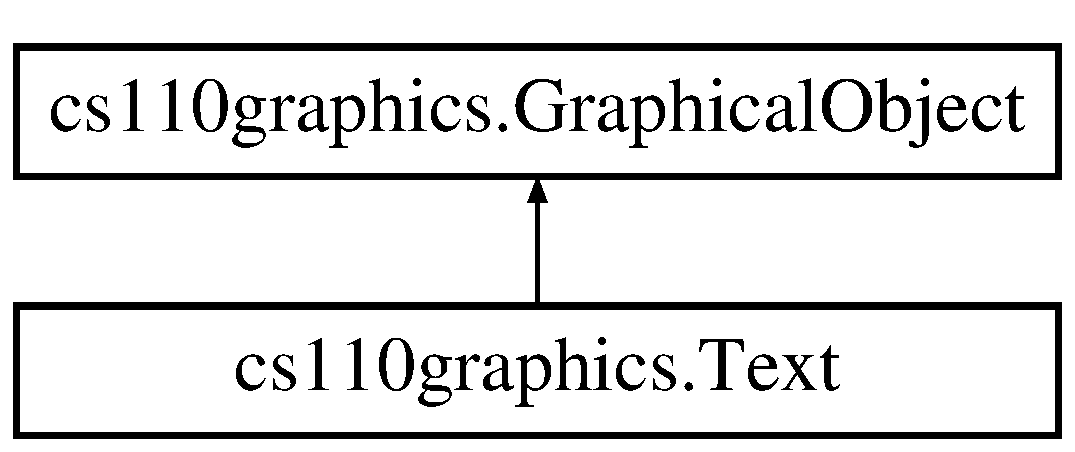
\includegraphics[height=2cm]{classcs110graphics_1_1Text}
\end{center}
\end{figure}
\subsection*{Public Member Functions}
\begin{DoxyCompactItemize}
\item 
def \hyperlink{classcs110graphics_1_1Text_a022ce78a2945edbd8dfe3c4498769a62}{\_\-\_\-init\_\-\_\-}
\item 
def \hyperlink{classcs110graphics_1_1Text_ad470aa26235fc2f5f1459c3750251207}{set\_\-size}
\begin{DoxyCompactList}\small\item\em Sets the font size of the text. \item\end{DoxyCompactList}\item 
def \hyperlink{classcs110graphics_1_1Text_ab12aa7478ca6a2b2015b7e8544674c73}{set\_\-text}
\begin{DoxyCompactList}\small\item\em Sets the text. \item\end{DoxyCompactList}\item 
def \hyperlink{classcs110graphics_1_1GraphicalObject_adb1af0d5a6baae3f9a08d21a3227c49f}{add\_\-handler}
\begin{DoxyCompactList}\small\item\em Adds a handler to the graphical object. \item\end{DoxyCompactList}\item 
def \hyperlink{classcs110graphics_1_1GraphicalObject_a062789c4cc9de38af32dcc4ff2058607}{get\_\-center}
\begin{DoxyCompactList}\small\item\em Returns the center of the object. \item\end{DoxyCompactList}\item 
def \hyperlink{classcs110graphics_1_1GraphicalObject_a6d9f5718cd0cf249e0d2842971bae17f}{get\_\-depth}
\begin{DoxyCompactList}\small\item\em Returns the depth of the object. \item\end{DoxyCompactList}\item 
def \hyperlink{classcs110graphics_1_1GraphicalObject_aa64d270fb83efa4a54e1a7953512f9cd}{move}
\begin{DoxyCompactList}\small\item\em Moves the object dx pixels horizontally and dy pixels vertically. \item\end{DoxyCompactList}\item 
def \hyperlink{classcs110graphics_1_1GraphicalObject_abe2d480265df7ac9447205c52c6946df}{move\_\-to}
\begin{DoxyCompactList}\small\item\em Moves a graphical object to a point. \item\end{DoxyCompactList}\item 
def \hyperlink{classcs110graphics_1_1GraphicalObject_a20d76d4ee4419c3065d61deb6cbc6700}{set\_\-depth}
\begin{DoxyCompactList}\small\item\em Sets the depth of the \hyperlink{classcs110graphics_1_1GraphicalObject}{GraphicalObject}. \item\end{DoxyCompactList}\end{DoxyCompactItemize}


\subsection{Detailed Description}
\hyperlink{classcs110graphics_1_1Text}{Text} which can be added to a \hyperlink{classcs110graphics_1_1Window}{Window} object. 

\subsection{Member Function Documentation}
\hypertarget{classcs110graphics_1_1Text_a022ce78a2945edbd8dfe3c4498769a62}{
\index{cs110graphics::Text@{cs110graphics::Text}!\_\-\_\-init\_\-\_\-@{\_\-\_\-init\_\-\_\-}}
\index{\_\-\_\-init\_\-\_\-@{\_\-\_\-init\_\-\_\-}!cs110graphics::Text@{cs110graphics::Text}}
\subsubsection[{\_\-\_\-init\_\-\_\-}]{\setlength{\rightskip}{0pt plus 5cm}def cs110graphics.Text.\_\-\_\-init\_\-\_\- ( {\em self}, \/   {\em window}, \/   {\em text}, \/   {\em size} = {\ttfamily 12}, \/   {\em center} = {\ttfamily (200,~200})}}
\label{classcs110graphics_1_1Text_a022ce78a2945edbd8dfe3c4498769a62}

\begin{DoxyParams}{Parameters}
\item[{\em window}]-\/ \hyperlink{classcs110graphics_1_1Window}{Window} -\/ the window which the object will be added to \item[{\em text}]-\/ str -\/ The text which is displayed \item[{\em size}]-\/ int -\/ {\bfseries (default: 12)} sets the size of the text \item[{\em center}]-\/ tuple of int $\ast$ int -\/ {\bfseries (default: (200, 200))} sets the center of the \hyperlink{classcs110graphics_1_1Image}{Image} \end{DoxyParams}


Reimplemented from \hyperlink{classcs110graphics_1_1GraphicalObject}{cs110graphics.GraphicalObject}.\hypertarget{classcs110graphics_1_1GraphicalObject_adb1af0d5a6baae3f9a08d21a3227c49f}{
\index{cs110graphics::Text@{cs110graphics::Text}!add\_\-handler@{add\_\-handler}}
\index{add\_\-handler@{add\_\-handler}!cs110graphics::Text@{cs110graphics::Text}}
\subsubsection[{add\_\-handler}]{\setlength{\rightskip}{0pt plus 5cm}def cs110graphics.GraphicalObject.add\_\-handler ( {\em self}, \/   {\em handler\_\-object})\hspace{0.3cm}{\ttfamily  \mbox{[}inherited\mbox{]}}}}
\label{classcs110graphics_1_1GraphicalObject_adb1af0d5a6baae3f9a08d21a3227c49f}


Adds a handler to the graphical object. 
\begin{DoxyParams}{Parameters}
\item[{\em handler\_\-object}]-\/ \hyperlink{classcs110graphics_1_1EventHandler}{EventHandler} -\/ the object that handles the events for this \hyperlink{classcs110graphics_1_1GraphicalObject}{GraphicalObject} \end{DoxyParams}
\hypertarget{classcs110graphics_1_1GraphicalObject_a062789c4cc9de38af32dcc4ff2058607}{
\index{cs110graphics::Text@{cs110graphics::Text}!get\_\-center@{get\_\-center}}
\index{get\_\-center@{get\_\-center}!cs110graphics::Text@{cs110graphics::Text}}
\subsubsection[{get\_\-center}]{\setlength{\rightskip}{0pt plus 5cm}def cs110graphics.GraphicalObject.get\_\-center ( {\em self})\hspace{0.3cm}{\ttfamily  \mbox{[}inherited\mbox{]}}}}
\label{classcs110graphics_1_1GraphicalObject_a062789c4cc9de38af32dcc4ff2058607}


Returns the center of the object. \begin{DoxyReturn}{Returns}
center -\/ tuple 
\end{DoxyReturn}
\hypertarget{classcs110graphics_1_1GraphicalObject_a6d9f5718cd0cf249e0d2842971bae17f}{
\index{cs110graphics::Text@{cs110graphics::Text}!get\_\-depth@{get\_\-depth}}
\index{get\_\-depth@{get\_\-depth}!cs110graphics::Text@{cs110graphics::Text}}
\subsubsection[{get\_\-depth}]{\setlength{\rightskip}{0pt plus 5cm}def cs110graphics.GraphicalObject.get\_\-depth ( {\em self})\hspace{0.3cm}{\ttfamily  \mbox{[}inherited\mbox{]}}}}
\label{classcs110graphics_1_1GraphicalObject_a6d9f5718cd0cf249e0d2842971bae17f}


Returns the depth of the object. \begin{DoxyReturn}{Returns}
depth -\/ int 
\end{DoxyReturn}
\hypertarget{classcs110graphics_1_1GraphicalObject_aa64d270fb83efa4a54e1a7953512f9cd}{
\index{cs110graphics::Text@{cs110graphics::Text}!move@{move}}
\index{move@{move}!cs110graphics::Text@{cs110graphics::Text}}
\subsubsection[{move}]{\setlength{\rightskip}{0pt plus 5cm}def cs110graphics.GraphicalObject.move ( {\em self}, \/   {\em dx}, \/   {\em dy})\hspace{0.3cm}{\ttfamily  \mbox{[}inherited\mbox{]}}}}
\label{classcs110graphics_1_1GraphicalObject_aa64d270fb83efa4a54e1a7953512f9cd}


Moves the object dx pixels horizontally and dy pixels vertically. 
\begin{DoxyParams}{Parameters}
\item[{\em dx}]-\/ int \item[{\em dy}]-\/ int \end{DoxyParams}
\hypertarget{classcs110graphics_1_1GraphicalObject_abe2d480265df7ac9447205c52c6946df}{
\index{cs110graphics::Text@{cs110graphics::Text}!move\_\-to@{move\_\-to}}
\index{move\_\-to@{move\_\-to}!cs110graphics::Text@{cs110graphics::Text}}
\subsubsection[{move\_\-to}]{\setlength{\rightskip}{0pt plus 5cm}def cs110graphics.GraphicalObject.move\_\-to ( {\em self}, \/   {\em point})\hspace{0.3cm}{\ttfamily  \mbox{[}inherited\mbox{]}}}}
\label{classcs110graphics_1_1GraphicalObject_abe2d480265df7ac9447205c52c6946df}


Moves a graphical object to a point. 
\begin{DoxyParams}{Parameters}
\item[{\em point}]-\/ tuple of (int $\ast$ int) \end{DoxyParams}
\hypertarget{classcs110graphics_1_1GraphicalObject_a20d76d4ee4419c3065d61deb6cbc6700}{
\index{cs110graphics::Text@{cs110graphics::Text}!set\_\-depth@{set\_\-depth}}
\index{set\_\-depth@{set\_\-depth}!cs110graphics::Text@{cs110graphics::Text}}
\subsubsection[{set\_\-depth}]{\setlength{\rightskip}{0pt plus 5cm}def cs110graphics.GraphicalObject.set\_\-depth ( {\em self}, \/   {\em depth})\hspace{0.3cm}{\ttfamily  \mbox{[}inherited\mbox{]}}}}
\label{classcs110graphics_1_1GraphicalObject_a20d76d4ee4419c3065d61deb6cbc6700}


Sets the depth of the \hyperlink{classcs110graphics_1_1GraphicalObject}{GraphicalObject}. 
\begin{DoxyParams}{Parameters}
\item[{\em depth}]-\/ int \end{DoxyParams}
\hypertarget{classcs110graphics_1_1Text_ad470aa26235fc2f5f1459c3750251207}{
\index{cs110graphics::Text@{cs110graphics::Text}!set\_\-size@{set\_\-size}}
\index{set\_\-size@{set\_\-size}!cs110graphics::Text@{cs110graphics::Text}}
\subsubsection[{set\_\-size}]{\setlength{\rightskip}{0pt plus 5cm}def cs110graphics.Text.set\_\-size ( {\em self}, \/   {\em size})}}
\label{classcs110graphics_1_1Text_ad470aa26235fc2f5f1459c3750251207}


Sets the font size of the text. 
\begin{DoxyParams}{Parameters}
\item[{\em size}]-\/ int \end{DoxyParams}
\hypertarget{classcs110graphics_1_1Text_ab12aa7478ca6a2b2015b7e8544674c73}{
\index{cs110graphics::Text@{cs110graphics::Text}!set\_\-text@{set\_\-text}}
\index{set\_\-text@{set\_\-text}!cs110graphics::Text@{cs110graphics::Text}}
\subsubsection[{set\_\-text}]{\setlength{\rightskip}{0pt plus 5cm}def cs110graphics.Text.set\_\-text ( {\em self}, \/   {\em text})}}
\label{classcs110graphics_1_1Text_ab12aa7478ca6a2b2015b7e8544674c73}


Sets the text. 
\begin{DoxyParams}{Parameters}
\item[{\em text}]-\/ str \end{DoxyParams}


The documentation for this class was generated from the following file:\begin{DoxyCompactItemize}
\item 
\hyperlink{cs110graphics_8py}{cs110graphics.py}\end{DoxyCompactItemize}

\hypertarget{classcs110graphics_1_1Timer}{
\section{cs110graphics.Timer Class Reference}
\label{classcs110graphics_1_1Timer}\index{cs110graphics::Timer@{cs110graphics::Timer}}
}


A class which continually runs a function after a delay.  
\subsection*{Public Member Functions}
\begin{DoxyCompactItemize}
\item 
def \hyperlink{classcs110graphics_1_1Timer_a7d40cc83eb4083d4afd97c3ce5279e1a}{\_\-\_\-init\_\-\_\-}
\item 
def \hyperlink{classcs110graphics_1_1Timer_aba0aae9c8bfff7c626112f0020383a8d}{set\_\-function}
\begin{DoxyCompactList}\small\item\em Sets the function which is going to be run. \item\end{DoxyCompactList}\item 
def \hyperlink{classcs110graphics_1_1Timer_ae176b030095b0d96fa0e91f2c398c40a}{set\_\-interval}
\begin{DoxyCompactList}\small\item\em Sets the interval between executions of the function. \item\end{DoxyCompactList}\item 
def \hyperlink{classcs110graphics_1_1Timer_afe14c3fd66571d0186a54a4075f31b7e}{start}
\begin{DoxyCompactList}\small\item\em Starts the timer. \item\end{DoxyCompactList}\item 
def \hyperlink{classcs110graphics_1_1Timer_a26ae5eb7c7da929f7e2b6e17e4b709b1}{stop}
\begin{DoxyCompactList}\small\item\em Stops the timer. \item\end{DoxyCompactList}\end{DoxyCompactItemize}


\subsection{Detailed Description}
A class which continually runs a function after a delay. 

\subsection{Member Function Documentation}
\hypertarget{classcs110graphics_1_1Timer_a7d40cc83eb4083d4afd97c3ce5279e1a}{
\index{cs110graphics::Timer@{cs110graphics::Timer}!\_\-\_\-init\_\-\_\-@{\_\-\_\-init\_\-\_\-}}
\index{\_\-\_\-init\_\-\_\-@{\_\-\_\-init\_\-\_\-}!cs110graphics::Timer@{cs110graphics::Timer}}
\subsubsection[{\_\-\_\-init\_\-\_\-}]{\setlength{\rightskip}{0pt plus 5cm}def cs110graphics.Timer.\_\-\_\-init\_\-\_\- ( {\em self}, \/   {\em window}, \/   {\em interval}, \/   {\em func})}}
\label{classcs110graphics_1_1Timer_a7d40cc83eb4083d4afd97c3ce5279e1a}

\begin{DoxyParams}{Parameters}
\item[{\em window}]-\/ \hyperlink{classcs110graphics_1_1Window}{Window} -\/ the window which the timer will use to start and stop the animation \item[{\em interval}]-\/ int -\/ the time (in milliseconds) that that the timer will wait \item[{\em func}]-\/ function -\/ the function which will be run \end{DoxyParams}
\hypertarget{classcs110graphics_1_1Timer_aba0aae9c8bfff7c626112f0020383a8d}{
\index{cs110graphics::Timer@{cs110graphics::Timer}!set\_\-function@{set\_\-function}}
\index{set\_\-function@{set\_\-function}!cs110graphics::Timer@{cs110graphics::Timer}}
\subsubsection[{set\_\-function}]{\setlength{\rightskip}{0pt plus 5cm}def cs110graphics.Timer.set\_\-function ( {\em self}, \/   {\em func})}}
\label{classcs110graphics_1_1Timer_aba0aae9c8bfff7c626112f0020383a8d}


Sets the function which is going to be run. 
\begin{DoxyParams}{Parameters}
\item[{\em func}]-\/ function \end{DoxyParams}
\hypertarget{classcs110graphics_1_1Timer_ae176b030095b0d96fa0e91f2c398c40a}{
\index{cs110graphics::Timer@{cs110graphics::Timer}!set\_\-interval@{set\_\-interval}}
\index{set\_\-interval@{set\_\-interval}!cs110graphics::Timer@{cs110graphics::Timer}}
\subsubsection[{set\_\-interval}]{\setlength{\rightskip}{0pt plus 5cm}def cs110graphics.Timer.set\_\-interval ( {\em self}, \/   {\em interval})}}
\label{classcs110graphics_1_1Timer_ae176b030095b0d96fa0e91f2c398c40a}


Sets the interval between executions of the function. 
\begin{DoxyParams}{Parameters}
\item[{\em interval}]-\/ int \end{DoxyParams}
\hypertarget{classcs110graphics_1_1Timer_afe14c3fd66571d0186a54a4075f31b7e}{
\index{cs110graphics::Timer@{cs110graphics::Timer}!start@{start}}
\index{start@{start}!cs110graphics::Timer@{cs110graphics::Timer}}
\subsubsection[{start}]{\setlength{\rightskip}{0pt plus 5cm}def cs110graphics.Timer.start ( {\em self})}}
\label{classcs110graphics_1_1Timer_afe14c3fd66571d0186a54a4075f31b7e}


Starts the timer. \hypertarget{classcs110graphics_1_1Timer_a26ae5eb7c7da929f7e2b6e17e4b709b1}{
\index{cs110graphics::Timer@{cs110graphics::Timer}!stop@{stop}}
\index{stop@{stop}!cs110graphics::Timer@{cs110graphics::Timer}}
\subsubsection[{stop}]{\setlength{\rightskip}{0pt plus 5cm}def cs110graphics.Timer.stop ( {\em self})}}
\label{classcs110graphics_1_1Timer_a26ae5eb7c7da929f7e2b6e17e4b709b1}


Stops the timer. 

The documentation for this class was generated from the following file:\begin{DoxyCompactItemize}
\item 
\hyperlink{cs110graphics_8py}{cs110graphics.py}\end{DoxyCompactItemize}

\hypertarget{classcs110graphics_1_1Window}{
\section{cs110graphics.Window Class Reference}
\label{classcs110graphics_1_1Window}\index{cs110graphics::Window@{cs110graphics::Window}}
}


\hyperlink{classcs110graphics_1_1Window}{Window} acts as a canvas which other objects can be put onto.  
\subsection*{Public Member Functions}
\begin{DoxyCompactItemize}
\item 
def \hyperlink{classcs110graphics_1_1Window_af926549e3d731847886302fa390f2863}{\_\-\_\-init\_\-\_\-}
\item 
def \hyperlink{classcs110graphics_1_1Window_a34064de02d5149841a23764e78085d18}{add}
\begin{DoxyCompactList}\small\item\em Adds an object to the \hyperlink{classcs110graphics_1_1Window}{Window}. \item\end{DoxyCompactList}\item 
def \hyperlink{classcs110graphics_1_1Window_a14aba875d32f8a70a0c5a80ac3f18a92}{remove}
\begin{DoxyCompactList}\small\item\em Removes an object from the \hyperlink{classcs110graphics_1_1Window}{Window} object, assuming the object being deleted exists. \item\end{DoxyCompactList}\item 
def \hyperlink{classcs110graphics_1_1Window_a2ab7070110bd58c95e8f29c10d71c7cc}{get\_\-height}
\begin{DoxyCompactList}\small\item\em Returns the height of the window as an integer. \item\end{DoxyCompactList}\item 
def \hyperlink{classcs110graphics_1_1Window_a41d27bb09f5033f0596af9f1a3a9b519}{get\_\-width}
\begin{DoxyCompactList}\small\item\em Returns the width of the window as an integer. \item\end{DoxyCompactList}\item 
def \hyperlink{classcs110graphics_1_1Window_a981a3115f1f22099549117313f38333c}{set\_\-background}
\begin{DoxyCompactList}\small\item\em Sets the background color of the canvas. \item\end{DoxyCompactList}\item 
def \hyperlink{classcs110graphics_1_1Window_a9b548549f8f09ca3f29e6e80483e21d2}{set\_\-height}
\begin{DoxyCompactList}\small\item\em Sets the height of the canvas. \item\end{DoxyCompactList}\item 
def \hyperlink{classcs110graphics_1_1Window_a227c806c2acbcaca9958ba3b610a85f6}{set\_\-title}
\begin{DoxyCompactList}\small\item\em Sets the title of the window holding the canvas. \item\end{DoxyCompactList}\item 
def \hyperlink{classcs110graphics_1_1Window_a55036373bfb4437eb4368a39fedb8722}{set\_\-width}
\begin{DoxyCompactList}\small\item\em Sets the width of the canvas. \item\end{DoxyCompactList}\end{DoxyCompactItemize}


\subsection{Detailed Description}
\hyperlink{classcs110graphics_1_1Window}{Window} acts as a canvas which other objects can be put onto. The standard size of window created by StartGraphicsSystem is width = 400, height = 400. 

\subsection{Member Function Documentation}
\hypertarget{classcs110graphics_1_1Window_af926549e3d731847886302fa390f2863}{
\index{cs110graphics::Window@{cs110graphics::Window}!\_\-\_\-init\_\-\_\-@{\_\-\_\-init\_\-\_\-}}
\index{\_\-\_\-init\_\-\_\-@{\_\-\_\-init\_\-\_\-}!cs110graphics::Window@{cs110graphics::Window}}
\subsubsection[{\_\-\_\-init\_\-\_\-}]{\setlength{\rightskip}{0pt plus 5cm}def cs110graphics.Window.\_\-\_\-init\_\-\_\- ( {\em self}, \/   {\em width}, \/   {\em height}, \/   {\em background}, \/   {\em name}, \/   {\em first\_\-function} = {\ttfamily None}, \/   {\em master} = {\ttfamily None})}}
\label{classcs110graphics_1_1Window_af926549e3d731847886302fa390f2863}

\begin{DoxyParams}{Parameters}
\item[{\em width}]-\/ int -\/ The width of the canvas \item[{\em height}]-\/ int -\/ The height of the canvas \item[{\em background}]-\/ str -\/ Background color of canvas. Can be either the name of a color (\char`\"{}yellow\char`\"{}), or a hex code (\char`\"{}\#FFFF00\char`\"{}) \item[{\em name}]-\/ str -\/ The title of the window \item[{\em first\_\-function}]-\/ proc(Window) -\/ {\bfseries (default: None)} When the window is created, it runs this function. \item[{\em master}]-\/ unkown type -\/ {\bfseries (default: None)} The parent widget. \end{DoxyParams}
\begin{DoxyWarning}{Warning}
Unless you understand how Tkinter works do not change master 
\end{DoxyWarning}
\hypertarget{classcs110graphics_1_1Window_a34064de02d5149841a23764e78085d18}{
\index{cs110graphics::Window@{cs110graphics::Window}!add@{add}}
\index{add@{add}!cs110graphics::Window@{cs110graphics::Window}}
\subsubsection[{add}]{\setlength{\rightskip}{0pt plus 5cm}def cs110graphics.Window.add ( {\em self}, \/   {\em graphic})}}
\label{classcs110graphics_1_1Window_a34064de02d5149841a23764e78085d18}


Adds an object to the \hyperlink{classcs110graphics_1_1Window}{Window}. 
\begin{DoxyParams}{Parameters}
\item[{\em graphic}]-\/ \hyperlink{classcs110graphics_1_1GraphicalObject}{GraphicalObject} \end{DoxyParams}
\hypertarget{classcs110graphics_1_1Window_a2ab7070110bd58c95e8f29c10d71c7cc}{
\index{cs110graphics::Window@{cs110graphics::Window}!get\_\-height@{get\_\-height}}
\index{get\_\-height@{get\_\-height}!cs110graphics::Window@{cs110graphics::Window}}
\subsubsection[{get\_\-height}]{\setlength{\rightskip}{0pt plus 5cm}def cs110graphics.Window.get\_\-height ( {\em self})}}
\label{classcs110graphics_1_1Window_a2ab7070110bd58c95e8f29c10d71c7cc}


Returns the height of the window as an integer. \begin{DoxyReturn}{Returns}
height -\/ int 
\end{DoxyReturn}
\hypertarget{classcs110graphics_1_1Window_a41d27bb09f5033f0596af9f1a3a9b519}{
\index{cs110graphics::Window@{cs110graphics::Window}!get\_\-width@{get\_\-width}}
\index{get\_\-width@{get\_\-width}!cs110graphics::Window@{cs110graphics::Window}}
\subsubsection[{get\_\-width}]{\setlength{\rightskip}{0pt plus 5cm}def cs110graphics.Window.get\_\-width ( {\em self})}}
\label{classcs110graphics_1_1Window_a41d27bb09f5033f0596af9f1a3a9b519}


Returns the width of the window as an integer. \begin{DoxyReturn}{Returns}
width -\/ int 
\end{DoxyReturn}
\hypertarget{classcs110graphics_1_1Window_a14aba875d32f8a70a0c5a80ac3f18a92}{
\index{cs110graphics::Window@{cs110graphics::Window}!remove@{remove}}
\index{remove@{remove}!cs110graphics::Window@{cs110graphics::Window}}
\subsubsection[{remove}]{\setlength{\rightskip}{0pt plus 5cm}def cs110graphics.Window.remove ( {\em self}, \/   {\em graphic})}}
\label{classcs110graphics_1_1Window_a14aba875d32f8a70a0c5a80ac3f18a92}


Removes an object from the \hyperlink{classcs110graphics_1_1Window}{Window} object, assuming the object being deleted exists. 
\begin{DoxyParams}{Parameters}
\item[{\em graphic}]-\/ \hyperlink{classcs110graphics_1_1GraphicalObject}{GraphicalObject} \end{DoxyParams}
\hypertarget{classcs110graphics_1_1Window_a981a3115f1f22099549117313f38333c}{
\index{cs110graphics::Window@{cs110graphics::Window}!set\_\-background@{set\_\-background}}
\index{set\_\-background@{set\_\-background}!cs110graphics::Window@{cs110graphics::Window}}
\subsubsection[{set\_\-background}]{\setlength{\rightskip}{0pt plus 5cm}def cs110graphics.Window.set\_\-background ( {\em self}, \/   {\em background})}}
\label{classcs110graphics_1_1Window_a981a3115f1f22099549117313f38333c}


Sets the background color of the canvas. 
\begin{DoxyParams}{Parameters}
\item[{\em background}]-\/ string -\/ Background color of canvas. Can be either the name of a color (\char`\"{}yellow\char`\"{}), or a hex code (\char`\"{}\#FFFF00\char`\"{}) \end{DoxyParams}
\hypertarget{classcs110graphics_1_1Window_a9b548549f8f09ca3f29e6e80483e21d2}{
\index{cs110graphics::Window@{cs110graphics::Window}!set\_\-height@{set\_\-height}}
\index{set\_\-height@{set\_\-height}!cs110graphics::Window@{cs110graphics::Window}}
\subsubsection[{set\_\-height}]{\setlength{\rightskip}{0pt plus 5cm}def cs110graphics.Window.set\_\-height ( {\em self}, \/   {\em height})}}
\label{classcs110graphics_1_1Window_a9b548549f8f09ca3f29e6e80483e21d2}


Sets the height of the canvas. 
\begin{DoxyParams}{Parameters}
\item[{\em height}]-\/ int \end{DoxyParams}
\hypertarget{classcs110graphics_1_1Window_a227c806c2acbcaca9958ba3b610a85f6}{
\index{cs110graphics::Window@{cs110graphics::Window}!set\_\-title@{set\_\-title}}
\index{set\_\-title@{set\_\-title}!cs110graphics::Window@{cs110graphics::Window}}
\subsubsection[{set\_\-title}]{\setlength{\rightskip}{0pt plus 5cm}def cs110graphics.Window.set\_\-title ( {\em self}, \/   {\em name})}}
\label{classcs110graphics_1_1Window_a227c806c2acbcaca9958ba3b610a85f6}


Sets the title of the window holding the canvas. 
\begin{DoxyParams}{Parameters}
\item[{\em name}]-\/ string \end{DoxyParams}
\hypertarget{classcs110graphics_1_1Window_a55036373bfb4437eb4368a39fedb8722}{
\index{cs110graphics::Window@{cs110graphics::Window}!set\_\-width@{set\_\-width}}
\index{set\_\-width@{set\_\-width}!cs110graphics::Window@{cs110graphics::Window}}
\subsubsection[{set\_\-width}]{\setlength{\rightskip}{0pt plus 5cm}def cs110graphics.Window.set\_\-width ( {\em self}, \/   {\em width})}}
\label{classcs110graphics_1_1Window_a55036373bfb4437eb4368a39fedb8722}


Sets the width of the canvas. 
\begin{DoxyParams}{Parameters}
\item[{\em width}]-\/ height \end{DoxyParams}


The documentation for this class was generated from the following file:\begin{DoxyCompactItemize}
\item 
\hyperlink{cs110graphics_8py}{cs110graphics.py}\end{DoxyCompactItemize}

\chapter{File Documentation}
\hypertarget{cs110graphics_8py}{
\section{cs110graphics.py File Reference}
\label{cs110graphics_8py}\index{cs110graphics.py@{cs110graphics.py}}
}


The main cs110graphics file.  
\subsection*{Classes}
\begin{DoxyCompactItemize}
\item 
class \hyperlink{classcs110graphics_1_1Window}{cs110graphics.Window}
\begin{DoxyCompactList}\small\item\em \hyperlink{classcs110graphics_1_1Window}{Window} acts as a canvas which other objects can be put onto. \item\end{DoxyCompactList}\item 
class \hyperlink{classcs110graphics_1_1Event}{cs110graphics.Event}
\begin{DoxyCompactList}\small\item\em An object representing an action from the user. \item\end{DoxyCompactList}\item 
class \hyperlink{classcs110graphics_1_1EventHandler}{cs110graphics.EventHandler}
\begin{DoxyCompactList}\small\item\em The \hyperlink{classcs110graphics_1_1EventHandler}{EventHandler} class should be extended by any class that reacts to user input in the form of some action with the computer mouse or the keyboard. \item\end{DoxyCompactList}\item 
class \hyperlink{classcs110graphics_1_1GraphicalObject}{cs110graphics.GraphicalObject}
\begin{DoxyCompactList}\small\item\em This is a parent class of any object which can be put into \hyperlink{classcs110graphics_1_1Window}{Window}. \item\end{DoxyCompactList}\item 
class \hyperlink{classcs110graphics_1_1Fillable}{cs110graphics.Fillable}
\begin{DoxyCompactList}\small\item\em This is a parent class of any object which can have its colors modified. \item\end{DoxyCompactList}\item 
class \hyperlink{classcs110graphics_1_1Image}{cs110graphics.Image}
\begin{DoxyCompactList}\small\item\em An image, which can be added to a \hyperlink{classcs110graphics_1_1Window}{Window} object. \item\end{DoxyCompactList}\item 
class \hyperlink{classcs110graphics_1_1Text}{cs110graphics.Text}
\begin{DoxyCompactList}\small\item\em \hyperlink{classcs110graphics_1_1Text}{Text} which can be added to a \hyperlink{classcs110graphics_1_1Window}{Window} object. \item\end{DoxyCompactList}\item 
class \hyperlink{classcs110graphics_1_1Polygon}{cs110graphics.Polygon}
\begin{DoxyCompactList}\small\item\em A \hyperlink{classcs110graphics_1_1Polygon}{Polygon}, which can be added to a \hyperlink{classcs110graphics_1_1Window}{Window} object. \item\end{DoxyCompactList}\item 
class \hyperlink{classcs110graphics_1_1Circle}{cs110graphics.Circle}
\begin{DoxyCompactList}\small\item\em A circle, which can be added to a \hyperlink{classcs110graphics_1_1Window}{Window} object. \item\end{DoxyCompactList}\item 
class \hyperlink{classcs110graphics_1_1Oval}{cs110graphics.Oval}
\begin{DoxyCompactList}\small\item\em An oval, which can be added to a \hyperlink{classcs110graphics_1_1Window}{Window} object. \item\end{DoxyCompactList}\item 
class \hyperlink{classcs110graphics_1_1Square}{cs110graphics.Square}
\begin{DoxyCompactList}\small\item\em A square, which can be added to a \hyperlink{classcs110graphics_1_1Window}{Window} object. \item\end{DoxyCompactList}\item 
class \hyperlink{classcs110graphics_1_1Rectangle}{cs110graphics.Rectangle}
\begin{DoxyCompactList}\small\item\em A rectangle, which can be added to a \hyperlink{classcs110graphics_1_1Window}{Window} object. \item\end{DoxyCompactList}\item 
class \hyperlink{classcs110graphics_1_1Timer}{cs110graphics.Timer}
\begin{DoxyCompactList}\small\item\em A class which continually runs a function after a delay. \item\end{DoxyCompactList}\end{DoxyCompactItemize}
\subsection*{Functions}
\begin{DoxyCompactItemize}
\item 
def \hyperlink{namespacecs110graphics_af1a7cabc9d0dea87259e97ad88ef85ac}{cs110graphics.StartGraphicsSystem}
\begin{DoxyCompactList}\small\item\em This initalizes the graphics system. \item\end{DoxyCompactList}\item 
def \hyperlink{namespacecs110graphics_a0715c42bb0e296007b96bd0a20903d16}{cs110graphics.RunWithYieldDelay}
\begin{DoxyCompactList}\small\item\em Begins an animation loop. \item\end{DoxyCompactList}\end{DoxyCompactItemize}


\subsection{Detailed Description}
The main cs110graphics file. 
\printindex
\end{document}
